\documentclass[12pt, oneside, a4paper]{scrbook}

%\VignetteIndexEntry{Meaningful aggregation and coercion of trajectory data in R} 

\usepackage[utf8]{inputenc} 
\usepackage[T1]{fontenc} 
\usepackage{indentfirst}
\usepackage{Sweave}

\usepackage[nottoc]{tocbibind} % adds entries for lof and lot to toc.
\usepackage{microtype} % avoid overfull boxes

\usepackage[section]{placeins} % keeps figures in its section


% Bibiliography:
\usepackage[authoryear]{natbib}
\bibliographystyle{apalike}
%\bibliographystyle{plainnat}


% Provide text formats for R code, packages, etc.
% from https://stat.ethz.ch/pipermail/r-help/2007-November/144810.html
\newcommand{\pkg}[1]{{\normalfont\fontseries{b}\selectfont #1}}
\let\proglang=\textsf
\let\code=\texttt
\newcommand{\codeintitles}[1]{{\tt #1}} % solves font problems in chapter / sections / etc. titles



%%%%%%%%%%%%%%%%%%%%%%%%%%%%%%%%%%%%%%%%%%%%%%%%%%%%%%%%%%%%%%%%%%
%%%%%%%%%%%%%%%%%%%%%%%%%%%%%%%%%%%%%%%%%%%%%%%%%%%%%%%%%%%%%%%%%%
%%%%%%%%%%%%%%%%%%%%%%%%%%%%%%%%%%%%%%%%%%%%%%%%%%%%%%%%%%%%%%%%%%


\begin{document}

\Sconcordance{concordance:trajagg.tex:trajagg.Rnw:%
1 791 1 1 3 5 0 1 2 28 1 1 4 2 1 1 7 2 1 1 2 1 0 2 1 %
5 0 1 1 5 0 1 1 5 0 1 1 11 0 1 2 29 1 1 3 2 0 1 1 5 0 %
1 1 5 0 1 1 5 0 1 1 10 0 1 2 27 1 1 3 2 0 1 1 5 0 1 2 %
12 0 1 2 173 1 1 4 8 0 2 1 5 0 1 3 1 0 1 1 5 0 1 3 1 %
0 1 1 5 0 1 5 3 0 1 2 1 0 2 1 5 0 1 4 2 0 3 1 5 0 1 3 %
1 0 1 1 13 0 1 2 61 1 1 4 8 0 3 1 5 0 1 3 6 0 2 1 5 0 %
1 3 6 0 2 1 6 0 1 2 44 1 1 3 7 0 1 3 1 0 1 1 5 0 1 3 %
1 0 1 1 5 0 1 1 6 0 1 3 1 0 1 1 10 0 1 2 9 1 1 3 5 0 %
1 2 2 1 1 2 4 0 1 2 2 1 1 3 5 0 1 2 2 1 1 2 4 0 1 2 %
27 1 1 4 3 0 1 1 5 0 1 3 1 0 1 1 5 0 1 3 1 0 1 1 6 0 %
1 2 13 1 1 4 163 1 1 2 1 0 2 1 13 0 1 2 29 1 1 3 5 0 %
1 2 6 1 1 2 6 0 1 1 6 0 2 1 7 0 1 1 5 0 1 1 6 0 1 1 5 %
0 1 1 6 0 1 1 7 0 1 2 8 1 1 16 1 2 34 1 1 2 7 0 1 2 8 %
1 1 2 1 0 1 1 5 0 1 1 13 0 1 2 7 1 1 3 2 0 1 1 18 0 1 %
2 16 1 1 3 24 0 1 2 14 1 1 3 16 0 1 2 9 1 1 4 9 0 1 2 %
31 1 1 5 4 0 1 1 6 0 1 3 6 0 1 3 1 0 1 3 1 0 2 1 6 0 %
1 2 10 1 1 6 5 0 1 1 5 0 1 3 1 0 1 2 6 0 1 3 6 0 1 2 %
1 0 1 3 1 0 1 2 1 0 1 2 7 0 1 2 13 1 1 3 7 0 1 1 8 0 %
1 3 8 0 1 4 10 0 1 2 16 1 1 3 2 0 1 5 3 0 1 1 5 0 1 1 %
8 0 1 2 12 1 1 4 3 0 1 1 6 0 1 3 16 0 1 4 12 0 1 2 8 %
1 1 3 2 0 1 6 5 0 1 2 6 0 1 1 8 0 1 2 24 1 1 2 19 0 1 %
2 31 1 1 5 6 1 1 29 50 1 1 4 3 0 1 1 5 0 2 1 5 0 1 1 %
7 0 1 2 9 1 1 10 1 2 10 1 1 4 3 0 2 1 5 0 1 1 9 0 1 2 %
9 1 1 11 1 2 60 1 1 4 3 0 1 3 2 0 1 1 3 0 1 2 10 1 1 %
14 1 2 19 1 1 2 10 0 1 2 60 1 1 5 4 0 1 5 3 0 1 4 2 0 %
1 3 6 0 1 3 11 0 1 2 22 1 1 27 1 2 25 1 1 3 2 0 1 7 5 %
0 1 3 6 0 1 7 5 0 1 3 7 0 1 1 6 0 1 1 7 0 1 2 15 1 1 %
42 1 39 52 1 1 3 2 0 1 3 6 0 1 3 1 0 2 1 5 0 1 3 1 0 %
1 1 9 0 2 1 5 0 1 1 5 0 1 4 2 0 1 3 9 0 1 2 15 1 1 5 %
4 0 1 3 6 0 1 7 5 0 1 3 6 0 1 3 7 0 1 3 13 0 1 1 13 0 %
1 2 19 1 1 36 1 2 24 1 1 3 2 0 1 3 1 0 1 1 1 4 2 0 1 %
5 3 0 1 9 7 0 1 7 5 0 1 2 5 0 1 2 13 0 1 2 14 1 1 15 %
1 2 232 1 1 3 2 0 1 1 5 0 2 1 6 0 1 1 7 0 1 2 6 1 1 4 %
3 0 1 13 12 0 1 3 1 0 2 1 1 5 3 0 1 2 6 0 1 1 5 0 1 1 %
6 0 1 1 7 0 1 2 36 1 1 4 3 0 1 1 5 0 2 1 5 0 1 3 1 0 %
1 1 5 0 1 3 1 0 1 2 6 0 1 2 6 0 1 2 1 0 1 2 6 0 1 4 8 %
0 1 2 1 0 1 2 6 0 1 3 1 0 1 1 5 0 1 3 1 0 1 2 6 0 1 4 %
7 0 1 5 8 0 1 5 3 0 1 2 1 0 1 1 1 4 2 0 2 1 1 3 1 0 1 %
1 6 0 1 2 14 1 1 4 8 0 1 2 1 0 1 1 5 0 1 3 1 0 1 1 5 %
0 1 1 5 0 1 1 5 0 1 3 6 0 2 1 5 0 1 3 6 0 1 1 5 0 1 1 %
5 0 1 3 1 0 1 2 6 0 1 3 6 0 2 1 5 0 1 2 6 0 1 2 6 0 1 %
3 8 0 1 2 11 1 1 3 2 0 1 1 5 0 1 3 1 0 1 1 5 0 1 3 6 %
0 1 2 6 0 1 1 5 0 1 1 5 0 1 2 6 0 1 2 6 0 1 2 6 0 1 8 %
6 0 1 1 5 0 1 1 6 0 1 3 1 0 1 1 10 0 1 2 12 1 1 4 3 0 %
1 1 5 0 1 4 7 0 1 8 6 0 1 1 5 0 1 3 1 0 1 1 5 0 1 1 5 %
0 1 3 1 0 1 1 5 0 1 3 7 0 1 2 52 1}



%%%%%%%%%%%%%%%%%%%%%%%%%%%%%%%%%%%%%%%%%%%%%%%%%%%%%%%%%%%%%%%%%%
%%% Title %%%
%%%%%%%%%%%%%%%%%%%%%%%%%%%%%%%%%%%%%%%%%%%%%%%%%%%%%%%%%%%%%%%%%%

\title{Meaningful aggregation and \\ coercion of trajectory data in \proglang{R}}
\subtitle{}
\author{\\ Roland Harhoff \\}
%\subject{}
%\publishers{}
\date{\today}

\maketitle

%%%%%%%%%%%%%%%%%%%%%%%%%%%%%%%%%%%%%%%%%%%%%%%%%%%%%%%%%%%%%%%%%%

\frontmatter

%%%%%%%%%%%%%%%%%%%%%%%%%%%%%%%%%%%%%%%%%%%%%%%%%%%%%%%%%%%%%%%%%%
%%% Abstarct %%%
%%%%%%%%%%%%%%%%%%%%%%%%%%%%%%%%%%%%%%%%%%%%%%%%%%%%%%%%%%%%%%%%%%
\chapter{Abstract}

\minisec{Background}
Nowadays an increasing amount of trajectory data with observed attribute values attached to the spatial positions of moving entities is generated.
Data aggregation is an useful and proposed technique to explore and analyse such data.
The \proglang{R} software environment provides solutions to handle and analyse spatial and spatio-temporal data.
The recently implemented \proglang{R} package \pkg{trajectories} supports the representation and analysis of trajectory data. 
It contains methods for a \textit{pure} spatial aggregation of trajectory point attribute data without respecting the trajectories' temporal characteristic.

\minisec{Aims}
This work aims to provide methods for meaningful overlay and (weighted) aggregation of trajectory data in \proglang{R} that respect the spatial and temporal domain.
The methods are supposed to be applicable to objects of classes defined in \pkg{trajectories} and to aggregate trajectory point attribute data over spatial and spatio-temporal grouping predicates represented by objects of classes defined in the packages \pkg{sp} and \pkg{spacetime}. 
Another aim is to provide methods for coercion of objects of classes that represent trajectories and that are defined in other \proglang{R} packages.

\minisec{Methods}
The implementation of the newly-created methods is guided by the implementation of methods for spatial and spatio-temporal overlay and aggregation from the packages \pkg{sp} and \pkg{spacetime}. 
In particular this regards the methods' arguments, that are also extended, as well as the data structures of the returned objects.

\minisec{Results}
Methods for meaningful spatial and spatio-temporal overlay and aggregation of \pkg{trajectories} objects are implemented by S4 generic functions and provided by the \proglang{R} package \pkg{trajaggr}.
The methods respect the spatial and temporal domain of the trajectory data and may be used with spatial or spatio-temporal grouping predicates. 
Weighted aggregation based on temporal or spatial characteristics of the trajectories is supported. 
Also methods for bidirectional coercion between objects representing trajectory data as well as for \textit{counting} of trajectories over spatial and spatio-temporal regions are provided.

\minisec{Conclusions}
The implemented aggregation methods provide a first basic approach to fill the gap in the lack of suitable software solutions for (weighted) aggregation of trajectory data in \proglang{R} that respect the data's spatial and temporal domain in a meaningful way.

%%%%%%%%%%%%%%%%%%%%%%%%%%%%%%%%%%%%%%%%%%%%%%%%%%%%%%%%%%%%%%%%%%

\tableofcontents

\listoftables
\begingroup
\let\clearpage\relax
\listoffigures
\endgroup

%%%%%%%%%%%%%%%%%%%%%%%%%%%%%%%%%%%%%%%%%%%%%%%%%%%%%%%%%%%%%%%%%%

\mainmatter

%\part{Theoretical part}


%%%%%%%%%%%%%%%%%%%%%%%%%%%%%%%%%%%%%%%%%%%%%%%%%%%%%%%%%%%%%%%%%%
%%% Introduction %%%
%%%%%%%%%%%%%%%%%%%%%%%%%%%%%%%%%%%%%%%%%%%%%%%%%%%%%%%%%%%%%%%%%%

\chapter{Introduction}

Currently there is lack of suitable software solutions in \proglang{R} regarding meaningful (weighted) aggregation of trajectory data with respect to the trajectories' spatial and temporal characteristics.
\par\medskip

Nowadays trajectory data with observed attribute values attached to the spatial positions of moving entities may be easily obtained, due to the further development of position tracking and parameter measuring sensors.
Thus an increasing amount of such trajectory data is available.
Due to the large amount of data techniques to explore, reduce and analyse these data are needed.
\par\medskip

Data aggregation in general is considered as a meaningful process for grouping large data sets \citep{goldstein_using_1994}, 
in which spatial and temporal grouping predicates are common \citep{fredrikson_temporal_1999}. 
\citet{meratnia_aggregation_2002} already proposed raster-based spatial and spatio-temporal aggregation for trajectory data.
And today it is generally accepted that aggregation is a useful process for exploration, reduction and analysis of trajectory data \citep{andrienko_exploratory_2003, giannotti_trajectory_2007, andrienko_spatial_2011}.
\par\medskip

The \proglang{R} software for statistical computing \citep{r_development_core_team_r:_2014} as an open source and widely used software environment provides various packages that support handling and analysing of spatial and spatio-temporal data.
In particular the recently implemented package \pkg{trajectories} \citep{pebesma_trajectories:_2014} supports the representation and analysis of trajectory data with the ability to distinguish between (sets of) trajectories of particular entities.
Regarding to aggregation the package \pkg{trajectories} provides methods performing a \textit{pure} spatial aggregation of trajectory point attribute data without respecting the temporal characteristic of the trajectories.
\par\medskip

The aim is to provide methods for meaningful overlay and aggregation of trajectory data in \proglang{R} that respect the spatial and temporal characteristics of the trajectories. The methods for overlay constitute the basis of the aggregation methods.

All methods are supposed to respect the characteristic of the sampling rate as well as the overall duration (or distance) based on the intersection of the trajectories with the geometries of the grouping predicate,
if several trajectories are involved.
In case of aggregation of one trajectory characterized by an irregular sampling rate a weighted aggregation approach is supported that weights the observed values according to the sampling rate.
In case of aggregation of several trajectories this approach may be extended by assigning weights to each particular trajectory, in which each weight corresponds to one particular geometry of the grouping predicate.

These weights are based on the duration (or distance) of that trajectory corresponding to its temporal (or spatial) intersection with the geometries of the grouping predicate.
\par\medskip

The implemented methods are supposed to be applicable to objects of classes defined in the package \pkg{trajectories} (\code{Track}, \code{Tracks}, \code{TracksCollection}) and to aggregate trajectory point attribute data over spatial and spatio-temporal grouping predicates represented by objects of classes defined in the packages \pkg{sp} \citep{pebesma_sp:_2014} and \pkg{spacetime} \citep{pebesma_spacetime:_2012}.
In particular the accepted spatial grouping predicates are supposed to be objects of the classes \code{SpatialPolygons}, \code{SpatialPixels} and \code{SpatialGrid} as well as their \code{data.frame} counterparts from the package \pkg{sp}.
For spatio-temporal grouping predicates objects of the classes \code{STF} and \code{STFDF} from the package \pkg{spacetime} are accepted.
\par\medskip

% Coercion
Besides the implementation of methods for bidirectional coercion between objects of classes defined in the packages \pkg{move} \citep{kranstauber_move:_2014} and \pkg{adehabitatLT} \citep{calenge_adehabitatlt:_2014} and objects of classes defined in the package \pkg{trajectories} are provided.
The classes from \pkg{move} and \pkg{adehabitatLT} are defined to represent animal trajectory data.
Due to the coercion methods the aggregation functionality is provided to trajectory data stored in objects of the classes defined in the mentioned packages. And vice versa data stored in \pkg{trajectories} objects may be analysed by methods provided by these packages.  Moreover the coercion provides access to a large amount of data stored in the movebank database \citep{wikelski_movebank:_2011}. This data is provided by objects whose classes are defined in the package \pkg{move}.
\par\medskip

% Count
Finally, an aim is to provide methods for counting the number of trajectories over spatial and spatio-temporal grouping predicates. Such methods may be used to analyse the spatial or spatio-temporal distribution of trajectories and are especially suitable for trajectories without attributes or for trajectories whose attributes may not be aggregated in a meaningful way.
\par\medskip

As pointed out the focus of this implementation is about aggregation over area-measured spatial or spatio-temporal grouping predicates.
It aims not for providing aggregation methods using temporal or cyclic temporal grouping predicates.
Also the aggregation of trajectory data by attributes is not part of this work.
Moreover an aggregation in terms of aggregating a set of trajectory points to a smaller set of points, what may be known as generalisation, is neither part of this work.
And finally no methods to aggregate trajectories connections, which are bounding in each case two consecutive trajectory points, are implemented.
\par\medskip

Generally the implemented methods for overlay and aggregation are guided by the implementation of the methods for spatial and spatio-temporal overlay and aggregation defined in the packages \pkg{sp} and \pkg{spacetime}.
Moreover the implemented methods are as far as possible consistent with the mentioned methods from \pkg{sp} and \pkg{spacetime} regarding to the methods' arguments and the data structure of the returned objects. The spatio-temporal overlay constitutes the basis of the aggregation methods.
\par\medskip

% S4 and generic
Regarding to the implementation itself all methods are defined by S4 generic functions and the entirety of the implemented methods as well as some example data from movebank are integrated in the \proglang{R} package \pkg{trajaggr}.  The package is developed with the current \proglang{R} version 3.1.2 (2014-10-31) \citep{r_development_core_team_r:_2014}. Even regarding to the coercion the methods are additionally defined by S4 generic functions, which enables an appropriate documentation as well as a comfortable usage.
\par\medskip

%Outline
This vignette is structured as follows: In Chapter~\ref{chap:stateoftheart} definitions for 'aggregation' and 'trajectory' are given and a review about the relevant literature and \proglang{R} packages is presented. In Chapter \ref{chap:meaningful} theoretical issues and considerations related to trajectories and its meaningful aggregation are introduced and the theoretical basics about the chosen realization of the aggregation is presented. In Chapter~\ref{chap:exampledata} the example data sets, that are provided with the created \proglang{R} package \pkg{trajaggr} and that are used for illustration purposes are introduced. In Chapter~\ref{chap:coercion} the implemented coercion methods are presented and illustrated. In Chapter~\ref{chap:overandaggregate} the implemented methods are introduced and illustrated by applying them to the example data sets. The method \code{over} may be used for spatial and spatio-temporal overlay with \code{Track} objects. The method \code{count} may be used to count the number of trajectories, and the method \code{aggregate} performs spatial and spatio-temporal aggregations of objects of the classes \code{Track}, \code{Tracks} and \code{TracksCollection}. In Chapter~\ref{chap:discussion} the strengths and weaknesses of the implemented methods are discussed. In Chapter~\ref{chap:conclusions} the results are summarized and evaluated, and the Chapter~\ref{chap:outlook} presents an outlook regarding to the weaknesses of the implementation and the remaining challenges related to meaningful aggregation of trajectory data.
\par\medskip



%%%%%%%%%%%%%%%%%%%%%%%%%%%%%%%%%%%%%%%%%%%%%%%%%%%%%%%%%%%%%%%%%%
%%% LitReview %%%
%%%%%%%%%%%%%%%%%%%%%%%%%%%%%%%%%%%%%%%%%%%%%%%%%%%%%%%%%%%%%%%%%%

\chapter{State of the Art}
\label{chap:stateoftheart}

%=====================================================================
% DEFINITIONS
%---------------------------------------------------------------------
\section{Definitions}
\label{sec:definitions}

\subsection*{Aggregation}

Data aggregation is a process deriving new data references, in which groups considered as wholes are created out of multiple original references \citep{andrienko2006exploratory}. The authors point out that there are numerous different techniques for data aggregation.
\par\medskip

\citet{stasch_meaningful_2014} define spatio-temporal aggregation as a process of grouping observations relative to spatial regions and/or temporal intervals, based on a spatial and/or temporal grouping predicate, with a subsequent calculation of statistical measures on the observed values in these groups of observations by applying an aggregation function.
The spatial regions and/or temporal intervals on which the groups are built represent the support of the aggregated values and indicate the change of support, which is typical for data aggregation.
\par\medskip

\subsection*{Trajectories}
The term 'Trajectory' is used in various different fields and disciplines and thus it is hard to give an overall general definition.
\par\medskip

\citet{roduit2009trajectory} defines trajectories as a continuous functions from \textit{R} to $R^n$, where $n$ represents the number of spatial dimensions.
In conjunction with movement data in the two dimensional space this function becomes $f(t) = [x, y]$, where $t$ corresponds to time and $x$ and $y$ are the coordinates of the point locations.
\par\medskip

Similarly but extended by attribute data trajectories are defined by \citet{stasch_meaningful_2014} as 'mappings from discrete objects and times to spatial locations', in which attribute data may be attached to the spatial locations.
\par\medskip


%=====================================================================
% LIT REVIEW
%---------------------------------------------------------------------
\section{Literature review - Aggregation of trajectory data}

One of the basic works about data aggregation comes from \citet{fredrikson_temporal_1999}. They introduce spatial and temporal aggregation as well as aggregation by attributes.
\par\medskip

Nowadays it is generally accepted that data aggregation is a meaningful process for grouping large data sets \citep{goldstein_using_1994}. 
Common aggregation approaches are using spatial and temporal grouping predicates \citep{fredrikson_temporal_1999}, and raster-based spatial and spatio-temporal aggregation are proposed for trajectories by \citet{meratnia_aggregation_2002}.
For instance with GPS sensors a large amount of spatio-temporal data is generated and aggregation is a useful approach for exploration and reduction of such data respectively of trajectory data \citep{andrienko_exploratory_2003, giannotti_trajectory_2007, andrienko_spatial_2011}.
\par\medskip

The authors N. Andrienko and G. Andrienko contributed a lot to the research about analysis of spatial and temporal data. They wrote a book about the exploratory analysis of such data \citep{andrienko2006exploratory}. 
Furthermore and in particular they worked on the visualisation of spatio-temporal (movement) data \citep{andrienko_exploratory_2003, andrienko2012visual} and also used aggregation techniques to support the visual exploration of such data \citep{andrienko2008spatio, andrienko2010general, andrienko_spatial_2011}. Moreover they worked on basic concepts of movement data and techniques to analyse it \citep{andrienko2008basic, andrienko2011conceptual}.
\par\medskip

There is just a very little further literature that explicitly examines the meaningfulness of spatio-temporal aggregation of trajectory data. A current work is that from \citet{stasch_meaningful_2014}, that examines meaningful spatial prediction and aggregation in general but also gives some statements about meaningful aggregation of trajectory data. See Section~\ref{sec:meaningfulissues} for further details.
\par\medskip

As examples of studies whose analyses are based on the aggregation of trajectory data one my refer to the studies from \citet{d2013participatory} and from \citet{elen2012aeroflex}. In the context of the latter study the authors used an appropriate measurement plan containing repeated measurements to guarantee a meaningful aggregation result. Moreover they stated that it is challenging to aggregate data in a meaningful way when the data is collected in an unstructured way.


%=====================================================================
% SOFTWARE REVIEW
%---------------------------------------------------------------------
\section{\proglang{R} packages}

The \proglang{R} software for statistical computing \citep{r_development_core_team_r:_2014} as an open source and widely used software environment provides rich packages that support handling and aggregation of spatial or temporal data (\pkg{sp} \citep{pebesma_sp:_2014}, \pkg{raster} \citep{hijmans_raster:_2014}, \pkg{zoo} \citep{zeileis_zoo:_2014} and \pkg{xts} \citep{ryan_xts:_2014}).
Additionally the package \pkg{spacetime} \citep{pebesma_spacetime:_2012} provides a first approach to fill the gap in the lack of suitable software solutions to analyse spatio-temporal data (\citet{schabenberger_statistical_2004} in \citet{pebesma_spacetime:_2012}). 
\par\medskip

The Comprehensive \proglang{R} Archive Network provides several packages that deal with trajectory data \citep{pebesma_cran_2014}. The packages \pkg{move} \citep{kranstauber_move:_2014}, \pkg{adehabitatLT} \citep{calenge_adehabitatlt:_2014} and \pkg{trip} \citep{sumner_trip:_2013} focus on animal trajectories. The package \pkg{spacetime} provides amongst others the class \code{STTDF} which is inspired by \pkg{adehabitatLT} \citep{bivand_applied_2008} and designed for trajectory data in general.
\par\medskip

The \pkg{move} package provides functions to access, analyse and download animal track data from the movebank database \citep{wikelski_movebank:_2011}. Three S4 classes (\code{Move}, \code{MoveBurst} and \code{MoveStack}) are defined to store movement data. These classes extend the class \code{SpatialPointsDataFrame}. 
\par\medskip

The package \pkg{adehabitatLT} provides a S3 class named \code{ltraj} that is defined as a list of \code{data.frame} objects each containing the data of one trajectory. The spatial and temporal information is \textit{simply} saved in columns of the \code{data.frame} objects.
\par\medskip

The \pkg{trip} package provides functions to access and manipulate animal tracking data that is stored in a S4 class called \code{trip}. The class \code{trip} as well extends the class \code{SpatialPointsDataFrame}.
\par\medskip

However only the package \pkg{spacetime} even supports spatio-temporal data handling and analysis including aggregation that respects the spatio-temporal characteristics of trajectory data.
\par\medskip

The package \pkg{spacetime} provides various S4 classes and methods for spatio-temporal data including generic aggregation functions that support spatial, temporal and spatio-temporal aggregation \citep{pebesma_spacetime:_2012}. The above mentioned class \code{STTDF}, designed for trajectory data, has amongst others a slot named \code{traj} that contains a list of \code{STI} objects each representing one trajectory.
The classes \code{STI} and its \code{data.frame} counterpart \code{STIDF} represent spatio-temporal irregular data, in which time and space points (of observed values) do not have an obvious organisation. Each value is stored in conjunction with its timestamp and its spatial feature (\code{STIDF}).
Two further classes and its \code{data.frame} counterparts are defined in \pkg{spacetime}: \code{STF} and \code{STS}. The class \code{STF} represents a spatio-temporal full grid. For each spatial feature the same temporal sequence is stored and analogous data is sampled in the case of its \code{data.frame} counterpart \code{STFDF}.
The class \code{STS} respectively the class \code{STSDF} represents a spatio-temporal sparse grid which has the same general layout as the class \code{STF}, yet not the full grid is stored but only observations with non-missing values.
\par\medskip

Methods for spatial or spatio-temporal overlays as defined in the packages \pkg{sp} \citep{pebesma_sp:_2014} and \pkg{spacetime} \citep{pebesma_spacetime:_2012} are the basis for aggregation methods for spatial or spatio-temporal data. 
In \pkg{sp} the overlay of spatial features and/or grids are defined to combine numerically two maps in which the \code{over} method retrieves indices or attributes from one spatial feature at the locations of another spatial feature \citep{bivand_applied_2008}.
In \pkg{spacetime} the method \code{over} is defined analogous to the definition in \code{sp} but relative to spatio-temporal data.
\par\medskip

Recently the author of \pkg{spacetime} provided the package \pkg{trajectories} \citep{pebesma_trajectories:_2014} that fits well into the special requirements of trajectory data. The package aims to fill the gap of missing generic data structures and methods for analysing trajectories with respect to space and time \citep{klus_analysing_2014}. The package provides a S4 class called \code{Track} that extends the class \code{STIDF} from \pkg{spacetime}. Additionally a slot named \code{connections} is part of the class definition to provide attribute data of the segments that connect two consecutive trajectory points. Two further S4 classes are implemented which represent a set of \code{Track} objects of one individual (\code{Tracks}) and a set of \code{Tracks} objects of different individuals (\code{TracksCollection}). The \pkg{trajectories} classes are enhanced versions of the class \code{STTDF} from \pkg{spacetime}.
Relating to aggregation there is just a spatial aggregation method implemented in \pkg{trajectories} yet which aggregates the trajectory points' data.
\par\medskip

%\minisec{Compare trajectories to move, adehabitatLT, etc}
Relative to the domains of space and time the classes representing trajectory data defined in the package \pkg{trajectories} are more \textit{powerful} than the classes defined packages \pkg{move}, \pkg{trip} and \pkg{adehabitatLT} as a result of extending the class \code{STIDF} from \pkg{spacetime}.
\par\medskip

%\minisec{Compare trajectories to spacetime}
Moreover \pkg{trajectories} classes are more \textit{powerful} in comparison to the class \code{STTDF} defined in \pkg{spacetime} because it provides the \code{connections} slot and the three classes introduced above. Improved are the representation and distinction of points and connections, as well as the ability to combine and to distinguish different trajectories of one individual (\code{Tracks}) and distinguish sets of trajectories of different individuals (\code{TracksCollection}). As yet just one aggregation method has been implemented which aggregates the trajectory points over space. 
\par\medskip


%%%%%%%%%%%%%%%%%%%%%%%%%%%%%%%%%%%%%%%%%%%%%%%%%%%%%%%%%%%%%%%%%%
%%% Meaningful %%%
%%%%%%%%%%%%%%%%%%%%%%%%%%%%%%%%%%%%%%%%%%%%%%%%%%%%%%%%%%%%%%%%%%

\chapter{Meaningfulness related to aggregation of trajectory data}
\label{chap:meaningful}

%\minisec{Meaningful intro}
This Chapter is divided into two sections. 
The first section explains which criteria are relevant related to a meaningful aggregation of trajectory data. 
The second section describes how some challenges derived from the criteria presented in the first Section are addressed.

\section{Issues about meaningful aggregation of trajectories}
\label{sec:meaningfulissues}

%\minisec{Section Intro: Issues related to aggregation of trajectory data}
The meaningfulness of aggregation of trajectory data depends on several criteria. The following list gives an overview and in the subsequent paragraphs these items are explained and discussed in detail. Important criteria are:

\begin{itemize}
\item the domains (space and/or time) represented by the grouping predicate, 
\item the target features whose data should be aggregated (points or segments) 
\item the measurement scales of the attributes to be aggregated, 
\item the choice of the aggregation function to be applied, 
\item the sampling rate of the trajectory data and its variability, 
\item the handling of irregular sampling rates (within one track) 
\item the approach to aggregate data (of several tracks) based on different sampling rates
\item the units of the attribute data (if having a spatial or temporal reference),  
\item the variability of the attribute data.
\end{itemize}

\par\medskip


\minisec{Grouping predicates}
Generally due to the spatio-temporal characteristic of trajectory data an aggregation process needs to respect the spatial as well as the temporal domain. 
In a meaningful aggregation one needs to keep the temporal and spatial information of the trajectory data. Due to the grouping predicate the temporal and/or spatial support of the (aggregated) data changes.
If the grouping predicate is based on spatio-temporal geometries the spatio-temporal support of the aggregated values is equivalent to these spatio-temporal geometries.
\par\medskip
If the grouping predicate represents for instance just the spatial domain, the spatial support of the aggregated values is again equivalent to the spatial geometries of the grouping predicate, but the temporal support of the data does not change, if one does not want to drop the temporal information completely.
This unchanged temporal information should be kept, because in a meaningful aggregation it is (normally) desired to keep all the available information of the data to be aggregated.
This results in a changed data structure that characterized by a spatial support equivalent to the spatial grouping predicate, whereas the temporal support keeps being unchanged and is equivalent to the track point timestamps.
Thus the resulting data structure may be characterized by one time series possibly of length zero for each spatial geometry from the spatial grouping predicate, in which the timestamps of the time series correspond to the track point timestamps.
\par\medskip
Moreover also other types of grouping predicates may be used. For instance temporal or cyclic temporal grouping predicates. Because these are not part of this work they are not further discussed in this context.
\par\medskip


\minisec{Target features}
In aggregation of trajectory data one needs to distinguish between the aggregation of point data corresponding to the trajectory points and \textit{connection} data corresponding to the segments connecting two consecutive track points.
If one aims to aggregate track point data there are no further issues or restrictions to be respected aside from the criteria represented in this section.
\par\medskip
In the case of aggregation of \textit{connection} data there are some further issues which need to be considered. If the grouping predicate contains more than one spatio-temporal geometry covering the whole spatio-temporal \textit{extent} of the trajectories whose data should be aggregated, some of the connections may intersect the spatial and/or the temporal borders of the spatio-temporal geometries.
Thus an adequate approach is needed to assign the data values corresponding to these connections to the spatio-temporal geometries intersected by these connections. 
\par\medskip
Another special situation appears, if the spatial domain of the grouping predicate is represented by \textit{complex} polygons and the aggregation of \textit{connection} data is desired. 
In such cases those connections, which intersect the spatial borders of spatio-temporal geometries, may intersect some of these geometries twice or several times, which need to be respected when assigning the data values corresponding to these connections to the spatio-temporal geometries.
\par\medskip


\minisec{Measurement scales and data types}

The ability to aggregate attribute data depends on the data types respectively of the measurement scales of the data. 
\citet{stevens_theory_1946} classified the measurement scales and permissible statistics, which may be applied in a meaningful manner to data corresponding to the defined scales. 
For instance the functions \textit{count} and \textit{mode} may be applied to all measurement scales.
The \textit{median} may be applied to the ordinal and higher scales, and the functions \textit{mean} and \textit{standard deviation} may be applied to the interval scale as well as to the ratio scale \citep{stevens_theory_1946}.
\citet{stasch_meaningful_2014} interpret the question of meaningfulness in a more specific way and introduce an approach in which a statistical operation on data is classified as meaningful, if the operation is 'interpretable in the context in which the data was generated'.
\par\medskip
Besides the scales introduced by \citet{stevens_theory_1946} there are further scales like for instance the cyclic scale corresponding to a direction of movement given in degree. But such a scale may be transformed to the nominal scale from Stevens. Thus Stevens measurement scales are not complete but well accepted.
\par\medskip


\minisec{Aggregation functions}

As stated in conjunction with the definition of aggregation in Section \ref{sec:definitions}
applying an aggregation function to a set of measurement values is the basis of an aggregation process.
Especially the usage of the function \textit{sum} in aggregation processes is problematic, which is known from the database community where it is referred to as the summarizability problem \citep{lenz_summarizability_1997, mazon_survey_2009}.
\par\medskip
\citet {stasch_meaningful_2014} pointed out that the function \textit{sum} can just be applied as an aggregation function in a meaningful way if the 'complete knowledge about the extent over which values are summed' is given.
That is not the case for trajectory data because we just have information about the parameter values at the track point locations where the data is measured, but not along the segments connecting the measurement points. 
Moreover if one aims to aggregate data of a trajectory there may be a lack of information about other entities which may move at the same time in the same spatial extent and which provide measurements of the same property as well.
\par\medskip
For completeness it should be mentioned that situations might occur in which the function \textit{sum} may be useful. For instance if one aims for counting of events or of a specific characteristic of a boolean variable a meaningful application of that function might be possible.
\par\medskip
Other (\textit{simple}) functions like the minimum or maximum of an attribute may be used as aggregation functions without any restrictions.
The usage of functions calculating a summary value considering several measurement values like the function  \textit{mean} is possibly not purely meaningful in all situations depending on the number of involved tracks and the characteristics of the sampling rates of the involved tracks as it is described in the following paragraphs. 
\par\medskip


\minisec{Sampling rate frequencies}

Generally it is desirable that the temporal (or spatial) frequency of the sampling rate should be high enough such that the time intervals (or distances) between two consecutive measurement points are smaller than the time intervals (or spatial extents) characterizing the spatio-temporal geometries of the grouping predicate.
That guarantees (at least for the temporal domain) that each spatio-temporal geometry intersected by the path of the track is (temporally) matched by at least one measurement point.
\par\medskip
The aim of data aggregation is to calculate one representative value for an attribute out of a set of values of that attribute for each unit of the grouping predicate.
An important point is the variability of the frequency of the sampling rate especially if an aggregation function like \textit{mean}, that calculates a new value considering several measurement values, is used. 
A track with a sampling rate with constant time intervals between all pairs of two consecutive measurements may be called a \textit{regular} trajectory and contrary a trajectory with a varying frequency of the sampling rate may be called an \textit{irregular} trajectory, in which meaningful analyses of the latter are more challenging \citep{calenge_concept_2009}.
\par\medskip
The measured data of each track point typically correspond to a particular time instance of the temporal domain in conjunction with a particular point of the spatial domain, and thus these measurement points itself do not have any duration or distance. 
But due to the movement of the tracked object and the permanent progression of time one may calculate duration and distance for each segment connecting two consecutive track points. 
For a regular trajectory with a sampling rate based for instance on time the durations corresponding to the segments are all equal.
So there is information about the attribute data related to the track points and information about duration and distance related to the connecting segments.
To combine these information one need to assign information about duration and distance to the measurements in a meaningful way.
\par\medskip
In case of a (temporal) regular trajectory the information about duration, if assigned to the measurement points, is equal for all points, and thus point data of such a regular trajectory may be aggregated without any restriction respectively without considering the duration assigned to the points.
The same applies to the aggregation of data from several regular trajectories if their sampling rate frequencies are equal (and their speed of movement is approximately similar).
\par\medskip
Assuming a (temporal) irregular trajectory in conjunction with the assignment of the varying duration from the sampling rate to the measurement points as described above one may need to respect this varying duration when calculating the representative aggregated value of an attribute. 
For instance the values, that got a long duration assigned, should have a higher impact to the representative aggregated value than corresponding values that got a short duration assigned.
Thus the sampling rate may need to be respected when aggregating data of an irregular trajectory. 
\par\medskip
The same applies to to the aggregation of several trajectories, independent if they are all regular with different sampling rates or if they are irregular. 
In both cases it is useful to respect the duration and/or distance. 
For instance in case of aggregation of several regular trajectories with different sampling rates with no respect of the duration those attribute values from trajectories with higher sampling rates would be overrepresented in the resulting aggregated value.
To clarify that one may assume two trajectories with different sampling rates following the same path and thus intersecting the same spatio-temporal geometries in the same way.
But due to the higher sampling rate of one trajectory more track points of that trajectory would intersect the spatio-temporal geometries, and when calculating the aggregated values for the spatio-temporal geometries more points of the high frequent sampled trajectory would contribute to the resulting value. 
This would not be meaningful because the two trajectories should contribute equally to a aggregated attribute value instead of assigning a higher importance to the high frequent sampled trajectory.
\par\medskip
Thinking further it may be desirable (in most cases) to have the ability to aggregate one or several trajectories with respecting the duration \textit{and} the distance assigned to the track points. 
If such an aggregation would be useful depends on the data to be aggregated and on the questions to be answered by the aggregation process. 
An example of such a situation, in which it would be highly desirable to respect the duration as well as the distance, is the aggregation of several (temporal) irregular trajectories, at which the individuals (or entities) are moving with highly different speed, for instance a mixture of trajectories from pedestrians and cars, whereas the measured data is independent from the speed itself.
Due to the temporal irregular sampling rate it would be desirable to respect the duration, and due to the highly different speed it would be desirable to respect the distance as well, because the fast individuals are passing the intersected spatio-temporal geometries faster and hence have on average less track points intersecting a particular spatio-temporal geometries than the slow individuals.
\par\medskip
The decision if it is useful to respect merely the information about duration or distance in the case of aggregation of at least one irregular trajectory may depend on several factors like the underlying question to be answered and the data to be aggregated and may be decided independently in every particular case.
But there are cases in which it is useful to respect merely duration or distance as described in the following paragraphs.
\par\medskip



\minisec{Spatial or temporal referenced data}

In cases where the units of the data to be aggregated have a temporal (or spatial) reference the additional information relative to duration (or distance) should be doubtlessly respected. A meaningful aggregation approach needs to respect the duration if the data units have a temporal reference or analogous the distance needs to be respected if the data units have a spatial reference.
\par\medskip
To illustrate that one may assume a trajectory of a motorized vehicle in conjunction with the measurement of the fuel consumption. 
The fuel consumption may be measured with reference to the driven distance for instance in litre per kilometre as well as with reference to the trip duration for instance in litre per hour.
Generally, when aggregating data, the resulting aggregated values have the same units as the input values but with a changed spatial and temporal support.
To meaningfully aggregate the consumption data given in litre per hour one need to respect the duration, that may be assigned to each measurement point like described above.
The aggregated values with measurement units of litre per hour correspond to data units and to the durations of the track passing each spatio-temporal geometry. 
For instance a certain measurement point got assigned the half of the time duration of the overall duration corresponding to the measurement points intersecting a particular spatio-temporal geometry. Then the value corresponding to that certain point needs to contribute to 50 percent to the resulting aggregated value, independently of the number of further measurement points intersecting that particular spatio-temporal geometry.
When aggregating attribute data with a spatial reference the distance assigned to the measurement points  needs to be respected analogously.
\par\medskip


\minisec{Data variability}
Moreover the variability of the data to be aggregated has an impact on the meaningfulness of aggregation in general. An aggregation result of a highly variable attribute need to be interpreted with caution as long as the frequency of the sampling rate is not high enough to catch the variability of the attribute.
\par\medskip



\section{Meaningful realization of aggregation}
\label{sec:meaningfulrealization}

This section describes how the challenges mainly derived from the criteria related to a trajectories sampling rate presented in Section~\ref{sec:meaningfulissues} are generally addressed by the approach of meaningful aggregation presented in this work.
The aggregation approach is based on a core assumption related to the trajectories sampling rates which is also explained in this Section.
\par\medskip


\minisec{Assigning duration and distance to track points}
The aggregation approach presented in this work uses the idea of assigning information about duration and distance of segments to track points, as it is mentioned in Section~\ref{sec:meaningfulissues} in the paragraphs about the sampling rate frequencies. 
This allows the combination of information about duration and distance corresponding to segments with the track points and consequential also with the measured data, and thus it allows a weighted aggregation of track point attribute data based on duration or distance assigned to these track points.
\par\medskip

Generally track points get the sum of the half of the duration and distance of their prior and subsequent segment assigned. 
But we have to take a closer look to track points whose prior and/or subsequent segment intersects the spatial or temporal border of spatio-temporal geometries of the grouping predicate, 
because such segments intersect (at least) two spatio-temporal geometries, and thus assigning information about duration and distance to that track points is not as simple as described above.
In particular one may want to calculate the exact duration and distance of the segment parts that intersect  the two spatio-temporal geometries, which are intersected by the two track points which define that segment, to obtain an adequate aggregation result in case of a applied weighted aggregation based on the assigned duration or distance.
\par\medskip

A general assumption is made to avoid the calculation of the exact duration and distance of the parts of segments intersected by a spatial or temporal border of the spatio-temporal geometries. 
It is assumed that the sampling rate of trajectories, which may be based on time or distance, is relatively high related to the time intervals or spatial extents of the grouping predicate. 
For instance a track sampling rate of one measurement per hour and a spatio-temporal grouping predicate with time intervals of 10 minutes would not meet that assumption. 
As a general rule related to time based sampling rates it is assumed that the sampling rate time intervals should at least be smaller than the time intervals defined in the spatio-temporal grouping predicate. 
\par\medskip

This assumption limits the maximal possible \textit{length} of the segments, in which length may be understood as spatial or temporal length.
Moreover it guarantees that those two consecutive points, which define a segment that intersects a spatial or temporal border of a spatio-temporal geometry of the grouping predicate, are intersecting two \textit{neighbouring} spatio-temporal geometries, in which \textit{neighbouring} means that these two spatio-temporal geometries have at least one \textit{corner point} in common.
\par\medskip

Consequential the assumption allows an adequate estimation of the duration and distance for segment parts by simply assigning the half of the segments duration and distance, because the possible error is limited by the controlled segments' \textit{length}. And basically the situation is as follows: The higher the frequency of the sampling rate the smaller is the possible error related to the estimation of duration and distance.
Finally these estimated values about duration and distance of the segments parts may be used to calculate the values of duration and distance which will be assigned to the corresponding track points.
\par\medskip


\minisec{Usage of assigned spatio-temporal information}
In the above paragraphs it is explained how information about duration and distance of segments is assigned in a meaningful manner to trajectory points to combine these spatio-temporal information with data corresponding to these trajectory points. This assigned spatio-temporal information is used in several ways.
\par\medskip

By providing the information about duration and distance corresponding to trajectory points a weighted aggregation of one trajectory over a spatial or spatio-temporal feature may be applied, in which the track point data may be weighted on basis of the information about duration and distance. This weighted approach may also be used when applying a map overlay of a spatio-temporal features and a trajectory. In any case of aggregation (or map overlay using an aggregation function) the information about duration and distance is used to calculate metadata about the approximate total duration and distance of track points respectively track \textit{parts} for each spatio-temporal geometry of the grouping predicate.
\par\medskip

Furthermore the calculated metadata may be used to perform a weighted aggregation of several trajectories, in which the track \textit {parts}, that intersect the same spatio-temporal geometry, are (additionally) weighted according to their duration or distance corresponding to that spatio-temporal geometry.
\par\medskip

\minisec{Other issues}
Generally this work just contains aggregation approaches which aggregate point data. Regarding to the grouping predicate the presented approaches keep the temporal and spatial information of the trajectories in any case. For further details see Section \ref{sec:generalaspects}.
An aggregation using the aggregation function \textit{sum}, which is typically not meaningful relative to trajectory aggregation, as it is described in Section~\ref{sec:meaningfulissues}, will be attended with a warning message.


%\part{Practical part}


%%%%%%%%%%%%%%%%%%%%%%%%%%%%%%%%%%%%%%%%%%%%%%%%%%%%%%%%%%%%%%%%%%
%%% ExData and Coercion %%%
%%%%%%%%%%%%%%%%%%%%%%%%%%%%%%%%%%%%%%%%%%%%%%%%%%%%%%%%%%%%%%%%%%


%=====================================================================
%=====================================================================
%
% CHAPTER Example data
%
%---------------------------------------------------------------------
%---------------------------------------------------------------------
\chapter{Example Data}
\label{chap:exampledata}

There are several example data sets provided with this package. 
Three data sets contain \pkg{move} objects from the movebank database \citep{wikelski_movebank:_2011}, and one data set contains an object of class \code{ltraj} defined in the package \pkg{adehabitatLT}. 
Additionally some artificial toy data containing objects whose classes are defined in \pkg{trajectories} as well as other spatial and spatio-temporal objects are provided (but not documented). 
\par\medskip

Moreover a function is provided which creates \code{SpatialPolygons}, \code{SpatialPixels} or a \code{SpatialGrid} object covering the extent of a \code{SpatialPoints} object that is passed to that function as the main argument.
This function and the toy data set are motivated and further introduced in the following paragraphs. The data sets from movebank and \pkg{adehabitatLT} are introduced in the subsequent sections.
\par\medskip

\minisec{Creation of \codeintitles{Spatial} grouping predicates}

The implemented methods expect as main arguments at least a \pkg{trajectories} object and an object inheriting from class \code{Spatial} or of class \code{STF} as the required grouping predicate. To illustrate the functionality of the implemented methods they are called with \pkg{trajectories} objects (coerced) from the example data sets introduced in this chapter. But adequate objects acting as grouping predicates of class \code{Spatial} or \code{STF} need to be created additionally. To simplify that creation process a function is implemented that creates area-measured \code{Spatial} objects from \code{SpatialPoints}. These created objects cover the whole extent of the passed \code{SpatialPoints}. This function is called \code{createSpatialArealObjFromPoints}. The desired dimension of the \textit{larger side} of the returned object as well as its desired class may be passed as optional arguments to the function.
\par\medskip

\minisec{Trajectories toy data}

The creation of the toy data was inspired by the implementation of \code{example("Track")} from the \pkg{trajectories} package \citep{klus_analysing_2014}, but it is built up of even more simple time and attribute data.
The data set contains several objects of classes defined in \pkg{trajectories} as well as other spatial and spatio-temporal objects which may be used as grouping predicates for the implemented methods. 
Objects from the toy dataset are used to illustrate the functionality of the method \code{over} in this vignette and to test the implemented methods related to the correctness of aggregated values using the package \pkg{testthat}. Moreover the data is used in some examples provided with the documentation.
For a detailed inspection of the two objects from the toy data set that are used in the calls of the method \code{over} see Section \ref{sec:overlaywithtrackobjects}.
The toy data set may be loaded by:
\par\medskip

% Load data
\begin{small}
\begin{Schunk}
\begin{Sinput}
> load(system.file("extdata","trajaggr_TestData.RData", 
+                  package = "trajaggr"), verbose = TRUE)
\end{Sinput}
\end{Schunk}
\end{small}

\par\medskip



%=====================================================================
% SECTION ExData movebank
%---------------------------------------------------------------------
\section{Example data from movebank}
\label{sec:exampledatamovebank}

\minisec{Vultures data set}

%original data
%Track4_X2, 37142 obs --> Tracks_X2 --> Torgos tracheliotus
%Track11_X1, 27116 --> Tracks_X1 --> Gyps africanus
%Track12_X3, --> Tracks_X3 --> Gyps africanus

The vultures data comes from a study about search efficiency of vultures foraging on spatio-temporally unpredictable carcasses in the Etosha National Park in Namibia \citep{spiegel_factors_2013, spiegel2014data}.
\par\medskip

The \code{MoveStack} object \code{vulture\_moveStack} represents a subset of the original data set downloaded from movebank and contains trajectory data of three vulture individuals, named X1 (\textit{Gyps africanus}), X2 (\textit{Torgos tracheliotus}) and X3 (\textit{Gyps africanus}). 
\par\medskip

The vultures were tracked in Namibia, in which this data subset covers a 14~days period. The daily tracking of the vultures was limited to the time interval from around 6 o'clock in the morning to 6 o'clock in the evening. The sampling rate is not regular and the time intervals between the relocations mainly vary between around 2 and 5 minutes. The data set contains 9639 tracked point locations and eleven attributes with values corresponding to the point locations, as it is shown by the following commands. The data set is loaded by \code{data(vulture\_moveStack)}:
\par\medskip


%' % Load required packages
%' \begin{small}
%' <<exampledata_load_pkgs, eval=TRUE, echo=FALSE>>=
%' #library(sp)
%' #library(spacetime)
%' #library(trajectories)
%' #library(trajaggr)
%' @
%' \end{small}


\begin{small}
\begin{Schunk}
\begin{Sinput}
> library(trajaggr)
> data(vulture_moveStack)
> class(vulture_moveStack)[1]
\end{Sinput}
\begin{Soutput}
[1] "MoveStack"
\end{Soutput}
\begin{Sinput}
> levels(vulture_moveStack@trackId)
\end{Sinput}
\begin{Soutput}
[1] "X1" "X2" "X3"
\end{Soutput}
\begin{Sinput}
> length(vulture_moveStack)
\end{Sinput}
\begin{Soutput}
[1] 9639
\end{Soutput}
\begin{Sinput}
> names(vulture_moveStack@data)
\end{Sinput}
\begin{Soutput}
 [1] "ground_speed"           "heading"               
 [3] "height_above_ellipsoid" "height_raw"            
 [5] "location_lat"           "location_long"         
 [7] "timestamp"              "visible"               
 [9] "sensor_type_id"         "deployment_id"         
[11] "event_id"              
\end{Soutput}
\end{Schunk}
\end{small}

\par\medskip

Due to the number of individuals and the characteristic of the data sampling this data sets needs some further preparation to be coerced to a \code{TracksCollection} in a suitable manner. This preparation is motivated and presented in Appendix \ref{sec:prepvulturemovestackforcount}.
\par\medskip

The permission to use the data was obtained from the owners of the data (Orr Spiegel).
Further information about the data set may be obtained by \code{?vulture\_moveStack}.
\par\medskip

%%%%%%%%

\minisec{Pigeons data sets}

The pigeons data come from a project, that studied the leadership-based flock structures of homing
pigeons (\textit{Columba livia}). In particular the repeatability of leadership-based flock structures was studied within a flight and across multiple flights conducted with the same animals \citep{santos2014data, santos_temporal_2014}.
\par\medskip

The pigeons data consist of overall four \code{MoveStack} objects. The objects represent already restructured subsets of the original data downloaded from movebank. Each of the \code{MoveStack} objects \code{pigeon\_R\_moveStack} and \code{pigeon\_S\_moveStack} contains two trajectories of one pigeon individual. In each case the trajectories of the two pigeon individuals are sampled regularly and synchronously and are following almost the same course. Each of the four trajectories corresponding to the mentioned objects contains 480 point locations tracked over a period of two minutes and thus the regular sampling rates have a very high frequency characterized by four samples per second. Nine data attributes whose values are corresponding to the tracked point locations are available for each of the trajectories.
\par\medskip

Additionally to these two introduced \code{MoveStack} objects equivalent but further limited objects are provided. Each trajectory represented by these objects is reduced to 60 point locations which corresponds to a sampling period of 15 seconds. These further reduced objects are named \code{pigeon\_R\_moveSt\_sub} and \code{pigeon\_S\_moveSt\_sub} and are used for illustration in Subsection \ref{subsec:aggregationbysp} due to the reduced required computation time according to the reduced number of point locations.
\par\medskip

For instance the data may be loaded by \code{data(pigeon\_R\_moveStack)}. The following commands give a short and exemplary inspecting of the \code{MoveStack} object \code{pigeon\_R\_moveStack}:
\par\medskip

\begin{small}
\begin{Schunk}
\begin{Sinput}
> # library(trajaggr)
> data(pigeon_R_moveStack)
> class(pigeon_R_moveStack)[1]
\end{Sinput}
\begin{Soutput}
[1] "MoveStack"
\end{Soutput}
\begin{Sinput}
> levels(pigeon_R_moveStack@trackId)
\end{Sinput}
\begin{Soutput}
[1] "R_17923536" "R_17923512"
\end{Soutput}
\begin{Sinput}
> length(pigeon_R_moveStack)
\end{Sinput}
\begin{Soutput}
[1] 960
\end{Soutput}
\begin{Sinput}
> names(pigeon_R_moveStack@data)
\end{Sinput}
\begin{Soutput}
[1] "comments"               "ground_speed"          
[3] "height_above_ellipsoid" "location_lat"          
[5] "location_long"          "timestamp"             
[7] "sensor_type_id"         "deployment_id"         
[9] "event_id"              
\end{Soutput}
\end{Schunk}
\end{small}

The permission to use the data was obtained from the owners of the data (Carlos David Santos). 
Further information about the data set may be obtained by the commands \code{?pigeon\_R\_moveStack} respectively \code{?pigeon\_S\_moveStack}. In the following Section \ref{sec:exampledataadehabitat} the example data from the package \pkg{adehabitatLT} is introduced.
\par\medskip



%=====================================================================
% SECTION ExData adehabitatLT
%---------------------------------------------------------------------
\section{Example data from the \proglang{R} package \pkg{adehabitatLT}}
\label{sec:exampledataadehabitat}

The package \pkg{trajaggr} contains one example data set of class \code{ltraj}, that is defined in the package \pkg{adehabitatLT}. The data set is stored in an object called \code{wildboars\_4Ind\_ltraj}.
\par\medskip

This data set is a modified version of the trajectory data stored in the object \code{puechabonsp}, which is provided by the \pkg{adehabitatLT} \citep{calenge_adehabitatlt:_2014}. The data represent the results of the monitoring of 4 wild boars in 1993 at Puechabon (Mediterranean habitat, South of France) and thus the original data contains four trajectories. The data set provided by the package \pkg{trajaggr} is modified in the way, that the trajectory of one individual is split (\textit{bursted}) into two trajectories respectively bursts. 
This provides a more complex structure relative to the number of trajectories corresponding to the individuals. Thus the provided data contains overall five trajectories of overall four individuals.
\par\medskip

The trajectories are characterized by a low frequent sampling rate with less than one tracked point location per day, as one may realize by inspecting the output of \code{summary} in the following block of commands. By \code{data(wildboars\_4Ind\_ltraj)} the data set may be loaded.
\par\medskip

\begin{small}
\begin{Schunk}
\begin{Sinput}
> # library(trajaggr)
> data(wildboars_4Ind_ltraj)
> class(wildboars_4Ind_ltraj)
\end{Sinput}
\begin{Soutput}
[1] "ltraj" "list" 
\end{Soutput}
\begin{Sinput}
> # library(adehabitatLT)
> adehabitatLT::summary.ltraj(wildboars_4Ind_ltraj)
\end{Sinput}
\begin{Soutput}
     id   burst nb.reloc NAs date.begin   date.end
1 Brock Brock.1       30   0 1993-07-01 1993-08-31
2 Calou Calou.1       19   0 1993-07-03 1993-08-31
3  Chou  Chou.1       16   0 1992-07-29 1992-08-28
4  Chou  Chou.2       24   0 1993-07-02 1993-08-30
5  Jean  Jean.1       30   0 1993-07-01 1993-08-31
\end{Soutput}
\end{Schunk}
\end{small}

\par\medskip

The \code{wildboars\_4Ind\_ltraj} data is just used for illustration of the methods that are implemented for coercion of objects of class \code{ltraj} to objects defined in \pkg{trajectories}.
The package \pkg{adehabitatLT} provides a lot of further example data sets.
\par\medskip

In the following Chapter \ref{chap:coercion} the implemented coercion methods are introduced and illustrated by being applied to the example data presented in this chapter.



%=====================================================================
%=====================================================================
%
% CHAPTER Coercion
%
%---------------------------------------------------------------------
%---------------------------------------------------------------------
\chapter{Coercion - Design and Implementation}
\label{chap:coercion}

%\minisec{Coercion Intro}
Methods are implemented that provide (mostly) bidirectional coercion between objects defined in the packages \pkg{move} and \pkg{adehabitatLT} and objects of the classes \code{Track}, \code{Tracks} or \code{TracksCollection} from the package \pkg{trajectories}.
\par\medskip

%\minisec{Generic coercion methods intro}
Generally coercion of an object \code{obj} may be applied by calling for instance \code{as(obj, "Track")}.
For all coercion methods generic coercion methods like \code{as.Track(obj)} are implemented as well. These generic methods enable easy usage of the coercion methods as well as an easy and appropriate documentation due to the fact that coercion methods are usually documented in conjunction with the documentation of the classes which are involved in the coercion.
\par\medskip

%\minisec{Coercion to \pkg{trajectories} objects and usage of \codeintitles{rbind.fill}}
In the cases of coercion of \code{Tracks} or \code{TracksCollection} objects the \code{data} slots of the involved \code{Track} objects are checked for consistency. If there are attributes which exist just in some \code{data} slots the slots are harmonized by using the function \code{rbind.fill} from the package \pkg{plyr}. 
Thus for such cases the package \pkg{plyr} is required. 
This functionality is implemented because there is no guarantee for identical structured \code{data} slots in \pkg{trajectories} objects (yet). The coercion related to objects defined in the package \pkg{move} is introduced in the Section~\ref{sec:coercionrelatedtomove}. The coercion related to \code{ltraj} objects defined in \pkg{adehabitatLT} is presented in Section~\ref{sec:coercionrelatedtoadeh}.
\par\medskip


%=====================================================================
% SECTION Coercion related to move
%---------------------------------------------------------------------
\section{Coercion related to objects defined in \pkg{move}}
\label{sec:coercionrelatedtomove}

A general overview of possible coercion options between objects defined in the packages \pkg{move} and \pkg{trajectories} is given by Table \ref{tab:possiblecoercion}. A coercion of \code{Track} objects to \code{MoveBurst} objects is obviously not possible because there is no information available on which the \code{Track} might be split into bursts of relocations.
\par\medskip

\begin{table}[!htb]
\centering
\begin{tabular}{lccc}
\hline\hline
Class & Track & Tracks & TracksCollection\\
\hline
Move & bidirectional & - & -\\
MoveBurst & Track & bidirectional & -\\
MoveStack & - & bidirectional & bidirectional\\
\hline\hline
\end{tabular}
\caption[Coercion between \pkg{move} and \pkg{trajectories} objects]{Possible coercion of objects defined in the packages \pkg{move} and \pkg{trajectories}. If not 'bidirectional' the possible direction of coercion is indicated by the class of the resulting object.}
\label{tab:possiblecoercion}
\end{table}

\par\medskip

By processing one of the coercion options shown in Table \ref{tab:possiblecoercion} the data from the \code{data} slot from e.g. a \pkg{move} object is passed to the \code{data} slot of the desired \pkg{trajectories} object and vice versa in the case of coercion in the contrary direction.
Furthermore each \pkg{move} object has a slot named \code{idData}. In cases of coercion to \code{Tracks} or \code{TracksCollection} objects the data from \code{idData} is passed to the \code{tracksData} or \code{tracksCollectionData} slot and as well vice versa in the case of coercion in the contrary direction.
Further details about the coercion related to \pkg{move} objects will be presented in the following subsections separated by the direction of coercion.

\par\medskip



%---------------------------------------------------------------------
% Coercion move --> traj
%---------------------------------------------------------------------
\subsection*{Coercion of objects defined in \pkg{move} to \pkg{trajectories} objects}
\label{subsec:coercemovetotraj}

%\minisec{Coercion of move objects intro}
\code{Move} objects will be coerced to \code{Track} objects and \code{MoveStack} objects may be coerced to \code{Tracks} or \code{TracksCollection} objects depending on the number of individuals involved. It is the responsibility of the user to choose the right coercion, because there is no way to definitely decide if the trajectories stored in a \code{MoveStack} object belong to a single individual or to several individuals. \code{MoveBurst} objects may be coerced to \code{Track} or \code{Tracks} objects.
\par\medskip

If a \code{Move} object is coerced to a \code{Track} object the information stored in the \code{idData} slot is lost. Moreover there are several other slots whose data is not passed to the desired \pkg{trajectories} object anyway. However this data may be classified as unimportant relating to trajectory data. For instance there is a slot \code{dateCreation} filled with an object of class \code{POSIXct} indicating the date of the data set creation.

\par\medskip


A special case is the coercion of \code{MoveBurst} objects to \code{Tracks}.
A \code{MoveBurst} object is similar to an object of class \code{Move} but is characterized by an additional slot named \code{burstId}. In this slot information is stored which is used to classify the segments connecting the consecutive points of an animal track. 
For instance the classification might be about the animals' behaviour, whereat each behavioural category could be specified and represented by an assigned particular character string. For each segment of the animal track one of these characterizing strings would be stored in the \code{burstId} slot.
Thus the \code{burstId} slot contains a vector whose length equals the number of track point minus one and whose elements define the classification of the segments (similar to the \code{connections} slot of a \code{Track} object).
\par\medskip
When coercing a \code{MoveBurst} to a \code{Tracks} object each set of consecutive segments belonging to the same classification category will be transformed to a particular \code{Track} object. 
To realize that those points with different \code{burstId} specifications corresponding to their prior and subsequent segments are duplicated, so that they may act as the last point of a \code{Track} representing a specific \code{burstId} category and at the same time as the first point of the next \code{Track} representing the following different \code{burstId} category.
Thus the resulting \code{Tracks} object contains in total more track points than the \code{MoveBurst}. This difference in the number of track points equals the number of sets of consecutive segments with a common \code{burstId} category minus one.
Due to the fact that the category of a set of consecutive segments do not have to be unique the resulting \code{Tracks} object may possess as well more \code{Track} objects than the number of classifying categories of the \code{MoveBurst}.

\par\medskip

The coercion of \pkg{move} objects to objects defined in \pkg{trajectories} is illustrated by the following commands which perform coercions of an object of class \code{MoveStack} to \code{Tracks} and \code{TracksCollection} objects as well as of an object of class \code{MoveBurst} to \code{Tracks}. Further validation of these coercions by comparing the relevant data (\code{data} and \code{idData} slots, coordinates and timestamps) may be found in Appendix \ref{sec:validmovecoercion}.


\begin{small}
\begin{Schunk}
\begin{Sinput}
> ### Coercion of MoveStack to Tracks
> # library(trajaggr)
> class(vulture_moveStack)[1]
\end{Sinput}
\begin{Soutput}
[1] "MoveStack"
\end{Soutput}
\begin{Sinput}
> v_Tracks <- as(vulture_moveStack, "Tracks")
> class(v_Tracks)[1]
\end{Sinput}
\begin{Soutput}
[1] "Tracks"
\end{Soutput}
\begin{Sinput}
> ## Compare as-method and generic method
> v_Tracks_gen <- as.Tracks(vulture_moveStack)
> identical(v_Tracks, v_Tracks_gen)
\end{Sinput}
\begin{Soutput}
[1] TRUE
\end{Soutput}
\begin{Sinput}
> ### Coercion of MoveStack to TracksCollection
> v_TrColl <- as.TracksCollection(vulture_moveStack)
> class(v_TrColl)[1]
\end{Sinput}
\begin{Soutput}
[1] "TracksCollection"
\end{Soutput}
\begin{Sinput}
> ### Coercion of MoveBurst to Tracks
> # Create a MoveBurst object from the first individuals' first day track
> # First subset the Move object to the first tracked day
> v_X1_Move <- vulture_moveStack[[1]]
> day1 <- which(as.Date(v_X1_Move@timestamps) == 
+                 as.Date(v_X1_Move@timestamps[1]))
> v_X1_1_Move <- v_X1_Move[day1]
> length(v_X1_1_Move) # number of locations
\end{Sinput}
\begin{Soutput}
[1] 189
\end{Soutput}
\begin{Sinput}
> # Create MoveBurst object with bursts specifying the type of 
> # locomotion (on.ground or flying) based on the vulture's speed
> behav <- rep("on.ground", length(day1))
> behav[which(v_X1_Move@data$ground_speed[day1] > 5)] <- "flying"
> v_X1_1_mb <- move::burst(v_X1_1_Move, f = behav[1:length(behav) - 1])
> length(v_X1_1_mb@burstId) # number of bursts corresponding to segments
\end{Sinput}
\begin{Soutput}
[1] 188
\end{Soutput}
\begin{Sinput}
> # Coerce MoveBurst to Tracks ...
> v_X1_1_mbTracks <- as.Tracks(v_X1_1_mb)
> v_X1_1_mbTracks@tracksData[c("n", "tmin", "tmax", "medspeed")]
\end{Sinput}
\begin{Soutput}
                  n                tmin                tmax
Burst1_on.ground 90 2008-05-02 06:03:59 2008-05-02 12:02:02
Burst2_flying    21 2008-05-02 12:02:02 2008-05-02 12:42:02
Burst3_on.ground 80 2008-05-02 12:42:02 2008-05-02 17:58:01
                    medspeed
Burst1_on.ground  0.03061205
Burst2_flying    15.95943986
Burst3_on.ground  0.01666610
\end{Soutput}
\end{Schunk}
\end{small}

\par\medskip

Related to the coercion of \code{MoveBurst} to \code{Tracks} objects we see from the commands above that the \textit{bursted} \code{Move} object contains 189 point locations.
By its coercion a \code{Tracks} object is created whose overall sum of \code{Track} points is 191. This information may be obtained by the returned \code{tracksData} which contains the attribute \code{n} specifying the number of point locations for each \code{Track} object. 
Moreover we see that the end time, indicated by \code{tmax}, for instance of the first \code{Track} and the start time of the second \code{Track} are identical.
The increased number of \code{Track} points and the identical timestamps indicate that two of the points of the original \pkg{move} object have been duplicated due to the implemented coercion method for coercing \code{MoveBurst} to \code{Tracks} as it is described above in detail. 

\par\medskip

We also see that the number of \code{Track} objects does not accord the number of \code{burst} categories. There are two \code{burst} categories, in particular "on.ground" and "flying", and the resulting \code{Tracks} object contains three \code{Track} objects (see \code{tracksData} output). That is the case because the \code{burstId} "on.ground" is used for two independent sets of consecutive segments which are transformed to two particular \code{Track} objects as described above. The Subsection \ref{subsec:coercetrajtomove} presents the contrary coercion of \pkg{trajectories} objects to \pkg{move} objects.



%---------------------------------------------------------------------
% Coercion traj --> move
%---------------------------------------------------------------------
\subsection*{Coercion of objects defined in \pkg{trajectories} to objects defined in \pkg{move}}
\label{subsec:coercetrajtomove}

A general overview of the options to coerce objects of class \code{Track}, \code{Tracks} and \code{TracksCollection} to objects of class \code{Move}, \code{MoveBurst} and \code{MoveStack} is given by Table~\ref{tab:possiblecoercion}. The method \code{move} from package \pkg{move} is used to create \code{Move} objects, which in turn optionally may be passed to the methods \code{move::burst} or \code{move::moveStack} to create objects of class \code{MoveBurst} or \code{MoveStack}.

\par\medskip

The \code{move} method has some specific characteristics which affect the coercion process.
The method expects besides the coordinates of the point locations, the information about the coordinates reference, the temporal information and the \code{data} corresponding to the locations also optionally two character strings, one to specify the used \code{sensor} and another representing the individual ID or name (\code{animal}), which are specified as 'unknown' and 'unnamed' by default.

\par\medskip

When creating a \code{Move} object using method \code{move} the passed character strings mentioned above are additionally stored in the \code{data} slot of the resulting object. Thus the \code{data} slot of a newly created \code{Move} object contains these two additional attributes not contained in the \code{data.frame} passed to the \code{data} argument of the \code{move} method.
This also applies in all implemented coercion methods of \pkg{trajectories} objects to \pkg{move} objects, and thus the \code{data} slots of the \code{Track} object and of the \code{Move} object are never identical due to the contained attribute columns.

\par\medskip

Moreover when creating a \code{Move} object by the method \code{move} attributes from the \code{data.frame}  passed to the \code{data} argument, whose parameter values are characterized by an overall identical singular value, are automatically stored in the \code{idData} slot of the resulting \code{Move} object instead of being stored in the \code{data} slot.
This characteristic is classified to be inadequate related to the coercion of \pkg{trajectories} objects to \pkg{move} objects, because on the one hand that data is related to the point locations and not to the individual even if the values are equal for all point locations, and on the other hand the \code{data} slot of the resulting object should contain (at least) all the attributes, which are contained by the \code{data} slot of the input object.
To realize an adequate coercion this characteristic behaviour of the \code{move} method is adjusted by the implementation of the coercion methods to get a desired adequate resulting object, whose \code{data} slot contains in any case all the attributes of the \code{data} slot of the input object.

\par\medskip

The coercion of \code{Tracks} to \code{MoveBurst} objects is a special case just as the contrary coercion described in the previous Subsection \ref{subsec:coercemovetotraj}.
Usually all point locations from the \code{Tracks} object are preserved and the points of the particular \code{Track} objects are concatenated to one (internal) \code{Move} object, which then is \textit{bursted} on basis of the particular \code{Track} objects respectively of their names. 
To realize that additional segments are needed to connect the sets of points of the particular \code{Track} objects.
These additional connections are not belonging clearly to one of the connected \code{Track} objects, and thus as well they are not belonging clearly to one of the \code{burst} categories, but however they need to get a \code{burst} category assigned.
Regarding to that problem an additional \code{burst} category named 'undefined' is assigned to these additional connecting segments. 
Thus the resulting \code{MoveBurst} contains one more \code{burst} category than the input \code{Tracks} object contains \code{Track} objects. 
Furthermore there is still one limitation related to this approach. In the input \code{Tracks} objects all \code{Track} objects have to be stored in chronological order.
\par\medskip

In special cases the \code{Tracks} object to be coerced may contain duplicated points (with identical timestamps) as end and start points of consecutive \code{Track} objects like it could be the case for instance if the object was created by coercion of a \code{MoveStack} object as it is described in the Subsection \ref{subsec:coercemovetotraj}.
Under these special conditions in each case of duplicated points one of these points will be deleted from the set of points which are be the basis for the creation of the \code{MoveStack} object.
Thus consecutive \code{Track} objects have theoretically one common point which acts as the end point for one \code{Track} object and concurrently acts as the start point of the subsequent \code{Track} object.
In this case the additional \code{burst} category 'undefined' is neither needed nor used.

\par\medskip

The coercion of \pkg{trajectories} objects to \pkg{move} objects is illustrated by the following commands coercing \code{Tracks} to \code{MoveStack} and \code{MoveBurst} objects as well as coercing a \code{TracksCollection} to a \code{MoveStack}. As input the \pkg{trajectories} objects created in Subsection \ref{subsec:coercemovetotraj} are used. The coercion is further validated in Appendix \ref{sec:validtrajtomovecoercion} by comparing the newly created \pkg{move} objects with the original \pkg{move} objects used as input for the coercion presented in Subsection~\ref{subsec:coercemovetotraj}.


\begin{small}
\begin{Schunk}
\begin{Sinput}
> ### Coercion of Tracks to MoveStack
> # library(trajaggr)
> class(v_Tracks)[1]
\end{Sinput}
\begin{Soutput}
[1] "Tracks"
\end{Soutput}
\begin{Sinput}
> library(move)
> v_moveSt <- as.MoveStack(v_Tracks)
> class(v_moveSt)[1]
\end{Sinput}
\begin{Soutput}
[1] "MoveStack"
\end{Soutput}
\begin{Sinput}
> ### Coercion of TracksCollection to MoveStack
> class(v_TrColl)[1]
\end{Sinput}
\begin{Soutput}
[1] "TracksCollection"
\end{Soutput}
\begin{Sinput}
> v_moveSt <- as.MoveStack(v_TrColl)
> class(v_moveSt)[1]
\end{Sinput}
\begin{Soutput}
[1] "MoveStack"
\end{Soutput}
\begin{Sinput}
> ### Coerce Tracks to MoveBurst
> class(v_X1_1_mbTracks)[1]
\end{Sinput}
\begin{Soutput}
[1] "Tracks"
\end{Soutput}
\begin{Sinput}
> v_X1_1_newMB <- as.MoveBurst(v_X1_1_mbTracks)
> class(v_X1_1_newMB)[1]
\end{Sinput}
\begin{Soutput}
[1] "MoveBurst"
\end{Soutput}
\end{Schunk}
\end{small}

\par\medskip

The commands above in conjunction with the validation in Appendix \ref{sec:validtrajtomovecoercion} verify the consistent coercion of \code{Tracks} and \code{TracksCollection} objects to objects defined in \pkg{move}. In the Section \ref{sec:coercionrelatedtoadeh} the coercion related to \code{ltraj} objects defined in the package \code{adehabitatLT} is presented.


%=====================================================================
% SECTION Coercion related to adehabitatLT
%---------------------------------------------------------------------
\section{Coercion related to \codeintitles{ltraj} objects defined in \pkg{adehabitatLT}}
\label{sec:coercionrelatedtoadeh}

%\minisec{Coercion ltraj intro}
Similar to the coercion of objects from \pkg{move} objects of class \code{ltraj} from \pkg{adehabitatLT} which will be coerced with respect to the number of IDs and bursts which are represented by the \code{ltraj} object. Due to the definitions of class \code{Track} in \pkg{trajectories} and of \code{burst} in \pkg{adehabitatLT} all coercion methods are built upon the determination that one \code{Track} corresponds to one \code{burst} and vice versa.

\par\medskip

The main part of the \code{ltraj} data corresponds to steps connecting two consecutive relocations and hence this data is stored in the \code{connections} slot(s) of the created objects defined in \pkg{trajectories}. The only exception is the attribute \code{R2n} which corresponds to the relocations and hence is stored accordingly. Moreover additional information related to the relocation may be stored in an object of class \code{ltraj}. In particular this data is stored in a \code{data.frame} saved as an \code{attribute} named \code{infolocs} for each burst of relocations. In case of coercion this data is stored in the \code{data} slot(s) of the returned \pkg{trajectories} object. All this described specifications are valid as well in the case of a vice versa coercion.

\par\medskip

Due to the fact that objects of class \code{ltraj} do not store any information about the coordinate reference system of the stored coordinates of the relocations, this information, if desired, needs to be set manually or gets lost dependent of the direction of the coercion.



%---------------------------------------------------------------------
% Coercion ade --> traj
%---------------------------------------------------------------------
\subsection*{Coercion of objects defined in \pkg{adehabitatLT} to \pkg{trajectories} objects}

Generally just \code{ltraj} objects with temporal information (indicated by the \code{attribute} \code{typeII}) may be coerced to \pkg{trajectories} objects. If \code{typeII == FALSE} the \code{ltraj} object does not have any temporal information related to the timestamps of the relocations. 
Another limitation regards the attributes \code{id} and \code{burst} in cases of coercion to \code{Track} or \code{Tracks} objects. In the former case neither the \code{id} nor the \code{burst} can be stored in the \code{Track} object. And in the latter case the \code{id} of the individual can not be stored in the \code{Tracks} object, whereas the \code{burst} character strings are stored as names for the \code{Track} objects being part of the \code{Tracks} object.
If a called coercion method is inadequate due to the desired class of the resulting object and the number of IDs and bursts of the passed object the evaluation of the method call is stopped. Examples of such cases are presented further down.
\par\medskip

%\minisec{NA in ltraj}
Objects of class \code{ltraj} tolerate NA values in the \code{data.frame} columns containing the spatial and temporal information. To realize a desired coercion the trajectory points with such missing information need to be dropped, because a \code{Track} object does not tolerate such missing values.
In such cases the \code{ltraj} data corresponding to the steps between relocations needs to be recalculated, which requires an installation of the package \pkg{adehabitatLT}. In all other cases \pkg{adehabitatLT} is not required.
\par\medskip

By the following commands the coercion of \code{ltraj} objects is illustrated by applying the coercion methods to the \code{ltraj} example data set \code{wildboars\_4Ind\_ltraj}. In Section \ref{sec:exampledataadehabitat} it is evaluated that the object \code{wildboars\_4Ind\_ltraj} is of class \code{ltraj} and contains altogether five busts of four individuals.
\par\medskip

\begin{small}
\begin{Schunk}
\begin{Sinput}
> # library(trajaggr)
> class(wildboars_4Ind_ltraj[1])
\end{Sinput}
\begin{Soutput}
[1] "ltraj" "list" 
\end{Soutput}
\begin{Sinput}
> # Coerce ltraj track of first individual (first burst) to Track object
> wb_1_Track <- as(wildboars_4Ind_ltraj[1], "Track")
> class(wb_1_Track)[1]
\end{Sinput}
\begin{Soutput}
[1] "Track"
\end{Soutput}
\begin{Sinput}
> # Coercion of third and fourth burst which belong to the same individual
> wb_Tracks <- as(wildboars_4Ind_ltraj[3:4], "Tracks")
> class(wb_Tracks)[1]
\end{Sinput}
\begin{Soutput}
[1] "Tracks"
\end{Soutput}
\begin{Sinput}
> dim(wb_Tracks)
\end{Sinput}
\begin{Soutput}
    tracks geometries 
         2         40 
\end{Soutput}
\begin{Sinput}
> # Coercion of whole ltraj object (4 ind., 5 bursts) to TracksCollection
> wb_TracksColl <- as(wildboars_4Ind_ltraj, "TracksCollection")
> wb_TracksColl@tracksCollectionData
\end{Sinput}
\begin{Soutput}
      n   xmin   xmax    ymin    ymax       tmin       tmax
Brock 1 698626 700387 3160768 3161559 1993-07-01 1993-08-31
Calou 1 699656 700419 3160553 3161678 1993-07-03 1993-08-31
Chou  2 699131 701410 3157848 3159572 1992-07-29 1993-08-30
Jean  1 699294 700306 3158012 3161450 1993-07-01 1993-08-31
\end{Soutput}
\end{Schunk}
\end{small}

\par\medskip
Further validation of the applied coercion is presented in Appendix \ref{sec:validltrajcoercion}.
The last output shows that the whole object \code{wildboars\_4Ind\_ltraj} may be coerced to a \code{TracksCollection} object. That object itself is composed of four \code{Tracks} objects whereas the third \code{Tracks} object contains two \code{Track} objects corresponding to the third and fourth burst from \code{wildboars\_4Ind\_ltraj} belonging to the individual \textit{Chou} (compare Section \ref{sec:exampledataadehabitat}).
By the following commands two examples of impossible coercion are shown.

\par\medskip

\begin{small}
\begin{Schunk}
\begin{Sinput}
> # Coercion of one burst to Tracks or TracksCollection is inadequate
> wb_1_Tracks <- as(wildboars_4Ind_ltraj[1], "Tracks")
\end{Sinput}
\end{Schunk}
\end{small}

\begin{small}
\begin{Schunk}
\begin{Soutput}
Error in asMethod(object) : length(from) > 1 is not TRUE!
\end{Soutput}
\end{Schunk}
\end{small}

\begin{small}
\begin{Schunk}
\begin{Sinput}
> # Coercion of bursts of several individuals to Tracks is inadequate
> wb_Tracks <- as(wildboars_4Ind_ltraj, "Tracks")
\end{Sinput}
\end{Schunk}
\end{small}

\begin{small}
\begin{Schunk}
\begin{Soutput}
Error in asMethod(object) : length(unique(idVec)) < 2 is not TRUE!
\end{Soutput}
\end{Schunk}
\end{small}

\par\medskip

In the following subsection the coercion of \pkg{trajectories} objects to objects of class \code{ltraj} is introduced and shortly illustrated by \textit{re-coercing} the above created objects back to \code{ltraj} objects. 

\par\medskip


%---------------------------------------------------------------------
% Coercion traj --> ade
%---------------------------------------------------------------------
\subsection*{Coercion of \pkg{trajectories} objects to objects defined in \pkg{adehabitatLT}}

Generally there are no further limitations in coercing \pkg{trajectories} objects to \code{ltraj} objects, but the package \pkg{adehabitatLT} is required in all cases.
The following commands illustrate the coercion to \code{ltraj} objects by coercing the above created \pkg{trajectories} objects back to objects of class \code{ltraj}. Further validation of the coercion may be found in Appendix~\ref{sec:validtrajtoltrajcoercion}.

\par\medskip

\begin{small}
\begin{Schunk}
\begin{Sinput}
> # Coercion of Track to ltraj
> # library(trajaggr)
> wb_1_ltraj <- as(wb_1_Track, "ltraj")
> class(wb_1_ltraj)
\end{Sinput}
\begin{Soutput}
[1] "ltraj" "list" 
\end{Soutput}
\begin{Sinput}
> # Coercion of Tracks to ltraj
> wb_3and4_ltraj <- as(wb_Tracks, "ltraj")
> class(wb_3and4_ltraj)
\end{Sinput}
\begin{Soutput}
[1] "ltraj" "list" 
\end{Soutput}
\begin{Sinput}
> # Coercion of TracksCollection to ltraj
> wb_ltraj <- as(wb_TracksColl, "ltraj")
> class(wb_ltraj)
\end{Sinput}
\begin{Soutput}
[1] "ltraj" "list" 
\end{Soutput}
\end{Schunk}
\end{small}

Aside from the mentioned limitations the output of the last command and the validation presented in Appendix~\ref{sec:validtrajtoltrajcoercion} show that the bidirectional coercion between \code{ltraj} objects and objects defined in \pkg{trajectories} preserves any relevant information. In the following Chapter \ref{chap:overandaggregate} the implemented methods \code{over}, \code{count} and \code{aggregate} are introduced and illustrated.




%%%%%%%%%%%%%%%%%%%%%%%%%%%%%%%%%%%%%%%%%%%%%%%%%%%%%%%%%%%%%%%%%%
%%% Aggregation %%%
%%%%%%%%%%%%%%%%%%%%%%%%%%%%%%%%%%%%%%%%%%%%%%%%%%%%%%%%%%%%%%%%%%


%=====================================================================
%=====================================================================
%
% CHAPTER Overlay and Aggregation
%
%---------------------------------------------------------------------
%---------------------------------------------------------------------
\chapter{Overlay and Aggregation - Design and Implementation}
\label{chap:overandaggregate}

%\minisec{Chapter Intro and outline}
This Chapter is about (map) overlay, counting of trajectories and aggregation of trajectory data represented by classes defined in the \proglang{R} package \pkg{trajectories}.
The Chapter starts with a description of general aspects related to the implemented methods \code{over}, \code{count} and \code{aggregate}. 
In the second Section the method \code{over} performing map overlays with \code{Track} objects is introduced in detail and applied to \code{Track} objects from the artificial toy data set introduced in Chapter \ref{chap:exampledata}.
In the Section~\ref{sec:count} the method \code{count} is presented and applied to \pkg{trajectories} objects created by coercion from the example \code{MoveStack} object \code{vulture\_moveStack}.
In the last Section of this Chapter the method \code{aggregate} is introduced and illustrated.
For illustration the method is applied to the example data objects \code{vulture\_moveStack}, \code{pigeon\_R\_moveSt\_sub} and \code{pigeon\_R\_moveSt\_sub}.
\par\medskip


\section{General aspects}
\label{sec:generalaspects}

This Section is about general aspects related to the implemented methods \code{over}, \code{count} and \code{aggregate}.
Generally the arguments which may be passed to the implemented methods are explained in conjunction with the illustration of these methods in the corresponding sections.
Besides the arguments already known from the methods \code{over} and \code{aggregate} implemented for objects of class \code{Spatial} and of classes defined in \pkg{spacetime} some additional arguments may be used when calling the methods \code{over} and \code{aggregate} for objects defined in \pkg{trajectories}.
These additional arguments, that may be used amongst others for attribute data selection and to perform weighted aggregations, are introduced in this Section.
\par\medskip
In conjunction with the arguments used to perform a weighted aggregation the general approach of the weighted aggregation is explained.
This Section contains moreover the description of the metadata provided by the results of any aggregation performed either by the method \code{over} or by the method \code{aggregate} and
a short introduction about the basic implementation approaches according to the class of the methods' grouping predicate.
Assumptions, that are (further) made related to the \pkg{trajectories} objects passed to the implemented methods, are introduced in the following paragraph.
\par\medskip


\minisec{Assumptions}
The implemented aggregation functionality is based on some core assumptions. We act on the assumption that the sampling rate of the \pkg{trajectories} objects is relatively high related to the time intervals or spatial extents of the grouping predicate. This assumption is introduced and motivated in detail in Section \ref{sec:meaningfulrealization}.
\par\medskip
Moreover it is generally assumed that the time reference of all \code{Track} objects that are themselves part of a \code{Tracks} or \code{TracksCollection} object is based on the same time zone.
This assumption is not (yet) a requirement related to the classes defined in \pkg{trajectories}.
\par\medskip


\minisec{Selection of attribute data}
The argument \code{use.data} may be used in the methods \code{over} and \code{aggregate}. When calling the method \code{over} \code{use.data} indicates whether the returned object contains (aggregated) data from the data slot of the \code{Track} object or indices of the \code{Track} points matching the spatio-temporal geometries passed to the \code{x} argument of the \code{over} method. If the default \code{use.data = FALSE} is used indices are returned. If \code{use.data = TRUE} (aggregated) data are returned. 
\par\medskip
To subset the attributes to be returned \code{over} may be called with passing an index \code{vector} or a character \code{vector} with the names of the desired columns to the \code{use.data} argument. The former selects the attribute columns in the \code{data} slot by the given indices whereas the latter selects attribute columns by the given names.
\par\medskip
For calls of the method \code{aggregate} the argument \code{use.data} needs to be \textit{positive}. Its default is \code{use.data = TRUE}, but analogous to the options defined for the method \code{over} particular attributes from the \code{data} slot of the \pkg{trajectories} objects may be selected by passing an index or a character \code{vector} to the \code{use.data} argument.
\par\medskip



\minisec{Metadata related to the aggregation result}
In conjunction with any aggregation either performed by the method \code{over} or by the method \code{aggregate} metadata for each geometry of the grouping predicate is provided.
The calculation of these metadata is (partly) based on the chosen approach to assign segments' durations and distances to the trajectory points as described in Section~\ref{sec:meaningfulrealization}. 
This metadata provides information about the approximate overall duration (\code{approx\_duration}) and distance (\code{approx\_distance}) assigned to the trajectory points respectively trajectory \textit{parts} spatio-temporally intersecting the particular geometries of the grouping predicate. 
Moreover the number of \code{Track} points intersecting each geometry (\code{nlocs}) as well as the number of \code{Track} objects (\code{ntraj}), if more than one \code{Track} is involved, are provided.
The metadata is stored as additional attributes in the \code{data.frame} respectively in the \code{data} slot of the object returned by called method.
\par\medskip


\minisec{Weighted aggregation}
% Pass a weighted aggregation function to over and aggregate
Besides the known arguments and functionality of \code{over} and \code{aggregate} methods from \pkg{sp} and \pkg{spacetime} the implemented methods for \pkg{trajectories} objects are extended with the possibility to pass a weighted aggregation function to the aggregation function argument \code{fn} respectively \code{FUN} to perform a weighted aggregation of \pkg{trajectories} object. Regarding the weighted aggregation function every built-in or user-defined function may be used, which expects a \code{vector} of weights as its second argument whereas the first argument specifies the data to be aggregated. For instance the function \code{weighted.mean} from the package \pkg{stats} as well as the function \code{weightedMedian} from the package \pkg{matrixStats} would be suitable.
\par\medskip

% Set the weight.points arg
The weighting of \code{Track} point attributes in the aggregation process may be performed using weights based on the duration or distance associated with the corresponding \code{Track} point. The approach to assign values about duration and distance to trajectory points is described in Section~\ref{sec:meaningfulrealization}.
The additionally provided argument \code{weight.points} is used to specify if the weights correspond to the assigned duration, specified by passing the \code{character} string 'byTime', or if the weights correspond to the assigned distance, specified by passing the \code{character} string 'byDist' to the \code{weight.points} argument.
\par\medskip

%weight.tracks
Besides the weighted aggregation of \code{Track} objects, where each \code{Track} point got a weight assigned, there is also the possibility to perform a weighted aggregation of \code{Tracks} or \code{TracksCollection} objects, in which furthermore each \code{Track} object may need to get a weight assigned. These weights are derived from the metadata containing information about the overall duration and distance of a \code{Track} object corresponding to each spatio-temporal geometry of the grouping predicate.
\par\medskip
Weights for the \code{Track} objects are specified by the additional argument \code{weight.tracks}, which expects just as the argument \code{weight.points} one of the character strings 'byTime' or 'byDist' to specify if the weights assigned to the \code{Track} objects are based on the overall duration or distance of that \code{Track} object corresponding to the spatio-temporal geometries of the grouping predicate. Typically both arguments should be specified equally.
\par\medskip
Thus for a weighted aggregation of a \code{Tracks} or \code{TracksCollection} object the arguments \code{weight.points} and \code{weight.tracks} both need to be specified, whereas in a first step a weighted aggregation of each particular \code{Track} specified by the \code{weight.points} argument is performed including the calculation of metadata about the overall duration and distance for each \code{Track}.
In the proximate step a weighted aggregation of the aggregation results from the first step is performed, in which the weights are specified by the argument \code{weight.tracks} and derived from the metadata calculated in the first step.
\par\medskip
To allow moreover a weighted aggregation of \code{Tracks} or \code{TracksCollection} objects in which weighting is limited to either just passing weights related to \code{Track} points or just passing weights related to \code{Track} \textit{parts} also the \code{character} string 'equal' may be passed to the arguments \code{weight.points} and \code{weight.tracks}. The string 'equal' indicates no weighting.
\par\medskip


\minisec{Applying aggregation functions individually}
When applying the methods \code{count} and \code{aggregate} to objects of class \code{TracksCollection} an additional argument named \code{byID} may be specified. 
This argument indicates if the called method is applied to the whole of the trajectories contained by the \code{TracksCollection}, which is the default case (\code{byID = FALSE}), or if the method is applied individually to the \code{Tracks} objects of the \code{TracksCollection}, which is the case if the method is called with \code{byID = TRUE}.
In the latter case the returned object contains for each (selected) attribute of the \code{TracksCollection} the individually aggregated attribute data for each \code{Tracks} object of the \code{TracksCollection} respectively for each tracked individual or entity. Just as the attribute data also the metadata is calculated individually for each \code{Tracks} object. To distinguish the returned data related to the particular individuals the \code{names} of the trajectory attributes as well as of the metadata attributes are extended by prefixing the \code{names} of the \code{Tracks} objects.
\par\medskip


\minisec{Approaches according to the methods' grouping predicate}
These paragraphs give a short introduction about the methods' implementation approaches according to the class of the methods' grouping predicate, whereat grouping predicate is meant to be the \code{x} argument of the \code{over} method or the \code{by} argument of the methods \code{count} and \code{aggregate}. The implemented methods accept two \textit{types} of grouping predicates. On the one hand objects of class \code{STF} or its \code{data.frame} counterpart and on the other hand \code{SpatialPolygons}, \code{SpatialPixels} and \code{SpatialGrid} objects as well as their \code{data.frame} counterparts are accepted.
\par\medskip
In the former case respectively if the grouping predicate is of class \code{STF} or its \code{data.frame} counterpart the returned object is of class \code{STFDF}, in which the spatio-temporal geometries correspond to the spatio-temporal geometries of the grouping predicate. 
That applies to all implemented methods.
The resulting attribute values, stored in the \code{data} slot of the \code{STFDF} object, are calculated for each geometry of the grouping predicate on the basis of those trajectories points spatio-temporally intersecting a particular geometry.
\par\medskip
In the latter case respectively if the grouping predicate is an object inheriting from class \code{Spatial} the situation is more complex.
As explained in Section \ref{sec:meaningfulissues} for instance in the case of aggregation one would expect something like one time series, for instance an \code{xts} object, possibly of length zero, for each spatial geometry from the \code{Spatial} grouping predicate, in which the timestamps of the time series correspond to the trajectory points' time instances.
But it is not possible to store a time series in a \code{Spatial} object in a comfortable and user-friendly way.
However as stated as well in Section \ref{sec:meaningfulissues} one wants to keep the temporal information definitely, and to realize that a \code{STFDF} object is chosen as the object to be returned if the method \code{aggregate} is called with a \code{Spatial} object grouping predicate.
\par\medskip
The \code{sp} slot of the returned \code{STFDF} object corresponds to the \code{Spatial} grouping predicate and the \code{time} slot is built out of the time instances of (the subset of) those trajectory points which are spatially intersecting the geometries of the grouping predicate.
Consequential in case of aggregation of a \code{Track} object each \code{Track} point intersecting the \code{Spatial} grouping predicate corresponds to its particular spatio-temporal geometry of the returned \code{STFDF} object. 
\par\medskip
Thus this approach is specially suitable to aggregate synchronously sampled trajectories, related to the aggregation of \code{Tracks} or \code{TracksCollection} objects, because in the case of non-synchronously sampled trajectories for each trajectory point a particular spatio-temporal geometry based on the timestamp of that point is created.
The same approach applies to the method \code{over}, in which the returned object is not of class \code{STFDF} but of one the typical classes returned by \code{over} depending on the method's arguments.
\par\medskip
For the method \code{count} the implementation approach is kept simple and in case of an object of class \code{Spatial} passed to the \code{by} argument an object of class \code{Spatial*DataFrame} is returned in which the temporal information of the \pkg{trajectories} object passed to \code{count} is ignored.
\par\medskip



%=====================================================================
% OVER
%---------------------------------------------------------------------
\section{\codeintitles{over} - Overlay with \codeintitles{Track} objects}
\label{sec:overlaywithtrackobjects}

%\minisec{Intro over methods}
The aim of the \code{over} method is to numerically combine two spatial or spatio-temporal features whereas indices or (aggregated) data of one feature corresponding to the (spatio-temporal) geometries of another feature are returned.
An overview of the available \code{over} methods related to \pkg{trajectories} classes could be obtained by the command \code{showMethods} whereas the required packages need to be loaded first, if not done yet:
\par\medskip

\begin{small}
\begin{Schunk}
\begin{Sinput}
> library(trajectories)
> library(trajaggr)
> showMethods(over, classes = c("Track", "Tracks", "TracksCollection"))
\end{Sinput}
\begin{Soutput}
Function: over (package sp)
x="SpatialGrid", y="Track"
x="SpatialPixels", y="Track"
x="SpatialPolygons", y="Track"
x="STF", y="Track"
x="TracksCollection", y="Spatial"
x="Track", y="Spatial"
x="Tracks", y="Spatial"
\end{Soutput}
\end{Schunk}
\end{small}

The output shows all available \code{over} methods related to the \pkg{trajectories} classes whereas the exported \code{over} methods from \pkg{trajaggr} are those whose signatures are characterized by \code{y="Track"}. 
Overlays for objects of class \code{STF} and for objects inheriting from class \code{Spatial} (\code{SpatialPolygons}, \code{SpatialGrid} and \code{SpatialPixels}) with objects of class \code{Track} are implemented.
\par\medskip

%\minisec{New over methods intro}
Generally the implemented \code{over} methods for spatial and spatio-temporal overlay are geared to the \code{over} methods implemented in \pkg{sp} and \pkg{spacetime} related to the arguments and the returned data structures. 
The methods respect the spatial and temporal domain of the \code{Track} object which will cause a consideration of the time domain even if an overlay of a \code{Spatial} object with a \code{Track} object is performed. 
\par\medskip

%\minisec{All incl additional arguments in new over methods}
Besides the arguments used by \code{over} implemented in \pkg{sp} and \pkg{spacetime} the \code{over} methods applying to \code{Track} objects 
are using the two further arguments \code{use.data} and \code{weight.points} which are introduced in Section \ref{sec:generalaspects}.
\par\medskip


%\minisec{Length of over return}
In general over(x, y) returns an object whose length equals \code{length(x)} if \code{x} is of or inherits from class \code{STF} or whose length equals \code{length(x) * length(y)} if \code{x} is of one of the classes mentioned above which inherit from class \code{Spatial} and all points from \code{y} are intersecting \code{x}.
\par\medskip

%\minisec{Toy data intro and loading}
For illustration of the \code{over} methods the small artificial toy data set is used, which easily allows to understand and verify the results of the implemented methods. 
For more details about that data set see Chapter \ref{chap:exampledata}. One may load that data set by:

% Load data
\begin{small}
\begin{Schunk}
\begin{Sinput}
> load(system.file("extdata","trajaggr_TestData.RData", 
+                  package = "trajaggr"), verbose = FALSE)
\end{Sinput}
\end{Schunk}
\end{small}

%\minisec{Inspecting toy data used for illustration of method over}
From the toy data set a \code{Track} object named \code{Track\_A1} and a \code{STF} object named \code{stf\_Polys\_4t} will (mainly) be used as input for the \code{over} methods.
Before applying \code{over} to the toy data objects we will inspect the properties of these objects including their dimensions and their temporal data to get a first rough idea of the expected results:

\begin{small}
\begin{Schunk}
\begin{Sinput}
> class(Track_A1)[1]
\end{Sinput}
\begin{Soutput}
[1] "Track"
\end{Soutput}
\begin{Sinput}
> dim(as(Track_A1, "STIDF"))
\end{Sinput}
\begin{Soutput}
    space      time variables 
        6         6         1 
\end{Soutput}
\begin{Sinput}
> library(spacetime)
> index(Track_A1@time) # Track point timestamps
\end{Sinput}
\begin{Soutput}
[1] "2012-12-20 01:00:00 CET" "2012-12-20 01:04:00 CET"
[3] "2012-12-20 01:16:00 CET" "2012-12-20 01:20:00 CET"
[5] "2012-12-20 01:24:00 CET" "2012-12-20 01:36:00 CET"
\end{Soutput}
\begin{Sinput}
> class(stf_Polys_4t)[1]
\end{Sinput}
\begin{Soutput}
[1] "STF"
\end{Soutput}
\begin{Sinput}
> dim(stf_Polys_4t)
\end{Sinput}
\begin{Soutput}
space  time 
    4     4 
\end{Soutput}
\begin{Sinput}
> class(stf_Polys_4t@sp)[1] # class of object in the sp slot
\end{Sinput}
\begin{Soutput}
[1] "SpatialPolygons"
\end{Soutput}
\begin{Sinput}
> index(stf_Polys_4t@time) # STF timestamps
\end{Sinput}
\begin{Soutput}
[1] "2012-12-20 01:00:00 CET" "2012-12-20 01:21:00 CET"
[3] "2012-12-20 01:42:00 CET" "2012-12-20 02:03:00 CET"
\end{Soutput}
\begin{Sinput}
> stf_Polys_4t@endTime # STF end times
\end{Sinput}
\begin{Soutput}
[1] "2012-12-20 01:21:00 CET" "2012-12-20 01:42:00 CET"
[3] "2012-12-20 02:03:00 CET" "2012-12-20 02:24:00 CET"
\end{Soutput}
\end{Schunk}
\end{small}

We see that the \code{Track} object contains six points and the \code{STF} object is built out of four \code{SpatialPolygons}. 
From the timestamps we may derive the information that the time of the \code{STF} object is considered to reflect time intervals, because the \code{endTime} values differ from the \code{time} values, and that all \code{Track} point time instances match one of the first two time intervals. Moreover one may notice that the sampling rate of the \code{Track} object is irregular, because the time differences between the \code {Track} point timestamps vary.
\par\medskip
Figure \ref{fig:tracka1pointsandpolygons} shows a visual (pure) spatial 'overlay' of the \code{Track} points and the \code{SpatialPolygons} from the \code{sp} slot of the \code{STF} object which further helps to understand the results of the up-coming \code{over} calls and which shows that the \code{SpatialPolygons} cover the whole spatial extent of the \code{Track} object.

\begin{figure}[!htb]
\centering
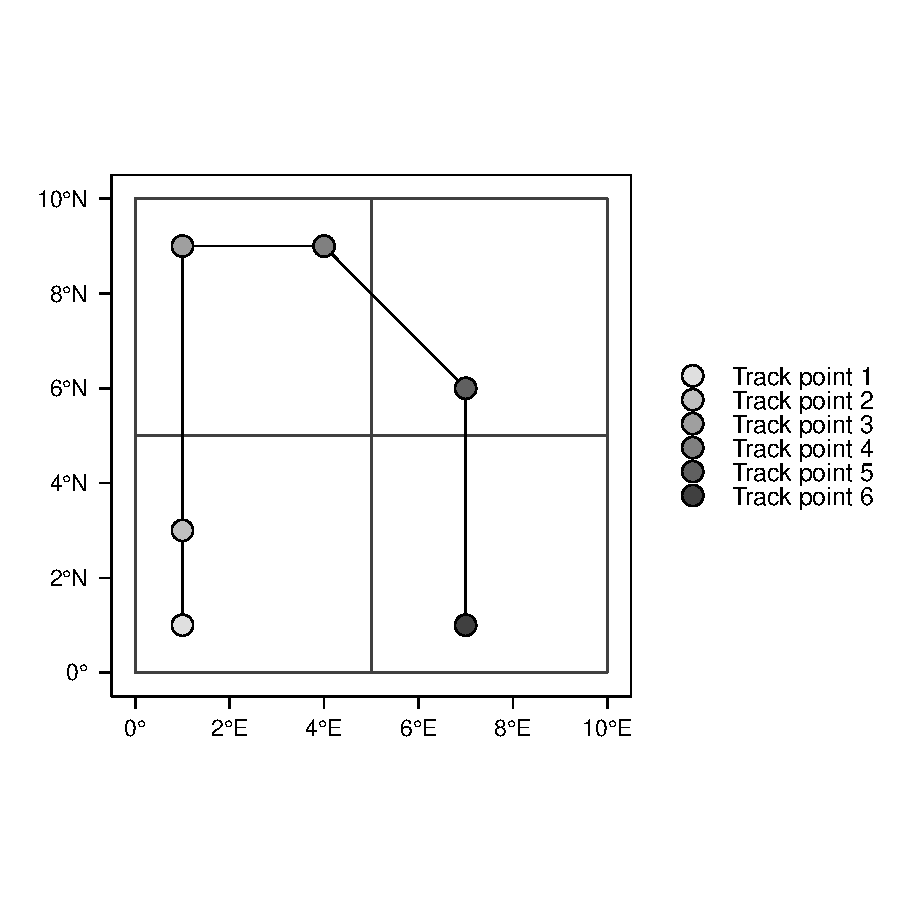
\includegraphics{trajagg-over_stf_inspect_byFig}
\caption[Spatial 'overlay' of example \code{Track} and polygons passed to \code{over.}]{Visual spatial 'overlay' of the example \code{Track} (\code{Track\_A1}) and the four \code{SpatialPolygons} (squares) from the \code{sp} slot of the \code{STF} object (\code{stf\_Polys\_4t}) that are passed to the \code{over} example calls.}
\label{fig:tracka1pointsandpolygons}
\end{figure}

\par\medskip

In the Subsection~\ref{subsec:overlayofstf} the usage and the results of the \code{over} method for spatio-temporal overlay of \code{STF} and \code{Track} objects are presented using the introduced toy data objects as input.


%---------------------------------------------------------------------
% Spatio-temporal overlay of STF and Track objects
%---------------------------------------------------------------------
\subsection{Overlay of \codeintitles{STF} and \codeintitles{Track} objects}
\label{subsec:overlayofstf}

%\minisec{First over call}
The spatio-temporal overlay of \code{STF} and \code{Track} objects performed by the method \code{over} returns \code{Track} point indices or (aggregated) \code{Track} attribute data for each spatio-temporal geometry of the \code{STF} object.
Calling the method \code{over} with the argument \code{returnList = FALSE} returns a \code{vector} of length \code{length(x)} with \code{Track} point indices:

\begin{small}
\begin{Schunk}
\begin{Sinput}
> over(x = stf_Polys_4t, y = Track_A1, returnList = FALSE)
\end{Sinput}
\begin{Soutput}
 [1]  3 NA  1 NA NA  5 NA  6 NA NA NA NA NA NA NA NA
\end{Soutput}
\end{Schunk}
\end{small}

Each \code{vector} element corresponds to one spatio-temporal geometry of the \code{STF} object and represents the index of the (first) corresponding \code{Track} point due to spatio-temporal intersection to that geometry. Due to the convention that spatial features are cycled first in \code{STF} objects \citep{pebesma_spacetime:_2012}, the first four \code{vector} elements represent the (first) indices of points that spatio-temporally intersect the four polygons during the first time interval of the \code{STF} object.
For instance the \code{Track} point number one (third \code{vector} element) intersects the third polygon during the first time interval, and the point number five (sixth \code{vector} element) intersects the second polygon during the second time interval. Moreover because there are no temporal matches between the \code{Track} point timestamps and the third and fourth time interval of the \code{STF} object, as we have seen above, the last eight \code{vector} elements just contain \code{NA} values.
\par\medskip
In the next command we change \code{returnList} to \code{TRUE} and a \code{list} of length \code{length(x)} is returned whereas each \code{list} element corresponds to one spatio-temporal geometry and contains the indices of all \code{Track} points corresponding to that geometry. 
Note that the printed output of the returned \code{list} is limited to a subset of the first three elements:

\begin{small}
\begin{Schunk}
\begin{Sinput}
> over_indexL <- over(x = stf_Polys_4t, y = Track_A1, returnList = TRUE)
> identical(length(stf_Polys_4t), length(over_indexL))
\end{Sinput}
\begin{Soutput}
[1] TRUE
\end{Soutput}
\begin{Sinput}
> over_indexL[1:3]
\end{Sinput}
\begin{Soutput}
[[1]]
[1] 3 4

[[2]]
integer(0)

[[3]]
[1] 1 2
\end{Soutput}
\end{Schunk}
\end{small}

The output shows that for instance the first polygon during the first time interval is intersected by the third and fourth \code{Track} point, which verifies and extends the information from Figure \ref{fig:tracka1pointsandpolygons} that the \code{Track} points three and four spatially intersect with the first, respectively the upper left, polygon.
\par\medskip
The \code{use.data} argument, whose default is \code{FALSE}, selects between returning indices, as it was shown above, and returning (aggregated) data. 
In the following command \code{use.data} and \code{returnList} are set to \code{TRUE} which causes the return of a \code{list} of \code{data.frame} objects whereas each \code{list} element represents again one spatio-temporal geometry of the \code{STF} object. The printed output is limited to the first three \code{list} elements again:

\begin{small}
\begin{Schunk}
\begin{Sinput}
> over_data <- over(x = stf_Polys_4t, y = Track_A1, returnList = TRUE,
+                  use.data = TRUE)
> over_data[1:3]
\end{Sinput}
\begin{Soutput}
[[1]]
  co2
3  12
4   4

[[2]]
[1] co2
<0 rows> (or 0-length row.names)

[[3]]
  co2
1   8
2   4
\end{Soutput}
\end{Schunk}
\end{small}

The printed part of the returned list shows the data values of the \code{Track} points intersecting the first three polygons and at the same time matching the first time interval of the \code{STF} object. In the case of no matches a \code{data.frame} with zero rows is returned as it is for the second \code{list} element.
\par\medskip
Relating to the \code{use.data} argument an integer or character \code{vector} may be passed to \code{use.data} as well to indicate that data should be considered and to select specific data columns at once, which is applied in the following two commands further down.
If concurrently to any \textit{positive} \code{use.data} argument \code{returnList} is set to \code{FALSE} a \code{data.frame} with \code{length(x)} rows will be returned. 
If the \code{fn} argument, whose default is \code{NULL}, keeps being unset each row of the returned \code{data.frame} contains the data of the first \code{Track} point that intersects the corresponding spatio-temporal geometry or \code{NA}, if there is no match. Moreover in the matching case the timestamp and the \code{timeIndex} of the (first) \code{Track} point is added to the \code{data.frame}. An example of such a call of the \code{over} method is presented in Subsection~\ref{subsec:overlayofspatial}.
\par\medskip
With the \code{fn} argument one may pass a built-in or user defined function to aggregate data by calculating summary statistics of data subsets.
In this case each row of the returned \code{data.frame} contains the aggregated data values of one spatio-temporal geometry instead of the data of the first matching \code{Track} point as described above.
\par\medskip
Additionally, if the \code{fn} argument is set, metadata about the number of relocations, the approximate duration and the approximate distance of the \code{Track} object are calculated for each spatio-temporal geometry. The estimated approximate values for duration and distance are calculated by summing the estimated values for each \code{Track} point intersecting the corresponding spatio-temporal geometry. The estimated point values are calculated by summing the half of the correspondent values of the \code{connections} which border on the corresponding \code{Track} point. See Section \ref{sec:meaningfulrealization} for further details.
\par\medskip

By adding \code{fn = mean} like in the following call of the \code{over} method mean attribute values are calculated. The returned \code{data.frame} contains the additional metadata represented by the variables \code{nlocs}, \code{approx\_duration} [sec] and \code{approx\_distance} [m]. The metadata are given in the same units as \code{duration} and \code{distance} in the \code{connections} slot of the \code{Track} object:

\begin{small}
\begin{Schunk}
\begin{Sinput}
> over(x = stf_Polys_4t, y= Track_A1, returnList = FALSE,
+      fn = mean, use.data = c(1))
\end{Sinput}
\begin{Soutput}
   co2 nlocs approx_duration approx_distance
1    8     2             720        895236.9
2   NA    NA              NA              NA
3    6     2             600        551981.3
4   NA    NA              NA              NA
5   NA    NA              NA              NA
6   12     1             480        510138.7
7   NA    NA              NA              NA
8    4     1             360        275980.0
9   NA    NA              NA              NA
10  NA    NA              NA              NA
11  NA    NA              NA              NA
12  NA    NA              NA              NA
13  NA    NA              NA              NA
14  NA    NA              NA              NA
15  NA    NA              NA              NA
16  NA    NA              NA              NA
\end{Soutput}
\end{Schunk}
\end{small}

Compared with the first and third \code{list} element returned by the presented command \\ \code{over(x = stf\_Polys\_4t, y = Track\_A1, returnList = TRUE, use.data = TRUE)} \\ one may recognize the accurate calculated mean values of the attribute \code{co2} in the first and third row of the recently returned \code{data.frame}. 
Because there are no temporal matches between the \code{Track} point timestamps and the third and fourth time interval of the \code{STF} object, as we have seen above already, the last eight rows of the \code{data.frame} just contain \code{NA} values.
\par\medskip
In the beginning of this Section we have seen that the sampling rate of the \code{Track} object \code{Track\_A1} is irregular. 
In such a case it might be useful to expand the calculation of summary statistics with a weighting procedure as it was explained in detail in Chapter~\ref{chap:meaningful}. 
The chosen approach is to weight the \code{Track} point attribute values according to the duration (or spatial distance) which may be assigned to each particular \code{Track} point. 
This weighting approach may be realized by passing a weighted aggregation function to the argument \code{fn} and concurrently passing an adequate \code{character} string to the \code{weight.points} argument, whose default is \code{NULL}. 
Currently the \code{weight.points} argument accepts the self-explanatory character strings 'byTime', 'byDist' and 'equal'.
\par\medskip
The following call of the method \code{over} illustrates this weighting approach by calculating means of the attribute value \code{co2} weighted by duration ('byTime'). 
Because we found out already that there are no matches between the \code{Track} points and the third and fourth time interval of the \code{STF} object, a subset of the \code{STF} object covering just the first and second time interval is passed to the \code{x} argument of the \code{over} method:

\begin{small}
\begin{Schunk}
\begin{Sinput}
> over(x = stf_Polys_4t[ , 1:2], y = Track_A1, returnList = FALSE, 
+      fn = weighted.mean, use.data = "co2", weight.points = "byTime")
\end{Sinput}
\begin{Soutput}
        co2 nlocs approx_duration approx_distance
1  9.333333     2             720        895236.9
2        NA    NA              NA              NA
3  4.800000     2             600        551981.3
4        NA    NA              NA              NA
5        NA    NA              NA              NA
6 12.000000     1             480        510138.7
7        NA    NA              NA              NA
8  4.000000     1             360        275980.0
\end{Soutput}
\end{Schunk}
\end{small}

Due to the subset of the \code{STF} object passed to \code{over} the returned \code{data.frame} just contains eight instead of 16 rows. 
We realize that the averaged \code{co2} values for the first and third spatio-temporal geometry of the \code{STF object}, respectively the first and third row of the returned \code{data.frame}, changed compared with the result of the prior unweighted call of the method \code {over}.
\par\medskip
The time differences between the second and the third as well as between the fifth and the sixth \code{Track} point timestamps are three times larger then the other time differences. 
This causes a higher contribution (in this particular case a doubled weight) of the attribute values of the four mentioned points to the weighted means calculated for the spatio-temporal geometries. 
For instance the weighted mean for the first spatio-temporal geometry is calculated by

\begin{small}
\begin{Schunk}
\begin{Sinput}
> (8 * 12 +   # contribution of the third Track point value (12), weight is 8
+  4 * 4) /   # contribution of the fourth Track point value (4), weight is 4
+  12         # sum of weights
\end{Sinput}
\begin{Soutput}
[1] 9.333333
\end{Soutput}
\end{Schunk}
\end{small}

Correspondingly the weighted mean for the third spatio-temporal geometry, which is intersected by the first two \code {Track} points, is smaller than the unweighted mean, because the smaller \code{co2} value of the second \code{Track} point gets the higher weight. 
There are no effects on the values for the sixth and eighth spatio-temporal geometry due to the fact that in each case just one \code{Track} point intersects these geometries, and as well there are no effects on the returned metadata, which is independent from the weighting procedure. 


%---------------------------------------------------------------------
% Overlay of Spatial and Track objects
\subsection{Overlay of \codeintitles{Spatial} and \codeintitles{Track} objects}
\label{subsec:overlayofspatial}

% DESCRIPTION how this over works ...
Due to the implementation approach of the method \code{over} for objects inheriting from class \code{Spatial} and \code{Track} objects, whose general aspects are explained in Section \ref{sec:generalaspects} in the paragraphs about the methods' grouping predicate, each element (or possibly row) of the returned data structure (\code{vector}, \code{list} or \code{data.frame}) contains the index or data of at most one \code{Track} point.
\par\medskip
Thus for all cases of spatial intersection of the \code{Track} points with the \code{Spatial} object calls of the method \code{over} with \code{returnList = TRUE} return the \textit{same} data (indices or attribute values) as calls with \code{returnList = FALSE}, whereas in the former case the data is returned as a \code{list} (possibly of \code{data.frame} objects) instead of a \code{vector} or \code{data.frame}.
\par\medskip
Moreover the \code{length} of the returned object depends on the number of \code{Track} points intersecting the \code{Spatial} object. If all points intersect the \code{Spatial} object the length of the returned object is \code{length(x)} * \code{length(y)}.
\par\medskip
These described characteristics will be illustrated by the following commands applying the \code{over} method with \code{use.data = FALSE}, which will cause the return of \code{Track} point indices:

\begin{small}
\begin{Schunk}
\begin{Sinput}
> ### over, in which all Track points intersect the Spatial object
> 
> # returnList = FALSE:
> over_sp <- over(x = stf_Polys_4t@sp, y = Track_A1, returnList = FALSE)
> over_sp
\end{Sinput}
\begin{Soutput}
 [1] NA NA  1 NA NA NA  2 NA  3 NA NA NA  4 NA NA NA NA  5
[19] NA NA NA NA NA  6
\end{Soutput}
\begin{Sinput}
> # Checking object length:
> identical(length(over_sp), length(stf_Polys_4t@sp) * length(Track_A1))
\end{Sinput}
\begin{Soutput}
[1] TRUE
\end{Soutput}
\begin{Sinput}
> # returnList = TRUE:
> over_sp_list <- over(x = stf_Polys_4t@sp, y = Track_A1, returnList = TRUE)
> # Checking if data is identical:
> bool_indices_1 <- !is.na(over_sp)
> bool_indices_2 <- sapply(over_sp_list, function(x) length(x) > 0)
> identical(over_sp[bool_indices_1], unlist(over_sp_list[bool_indices_2]))
\end{Sinput}
\begin{Soutput}
[1] TRUE
\end{Soutput}
\end{Schunk}
\end{small}

The result of the above first \code{over} call with \code{returnList = FALSE} need to be interpreted as follows: 
The returned \code{vector} of indices has the length \code{length(x)} * \code{length(y)} and corresponds to a theoretical non-existent \code{STF} object which would be built up out of the \code{Spatial} object passed to the \code{x} argument and out of the time instances of the \code{Track} points spatially intersecting the \code{Spatial} object, whereas in this particular case all \code{Track} points, respectively their time instances, would be considered.
This implies that the first four elements of the returned \code{vector} correspond to the four polygons at the time instance of the first \code{Track} point and that this \code{Track} point intersects the third polygon. 
Analogous we may realize that the second \code{Track} point as well intersects the third polygon, but at the time instance of the second \code{Track} point, and the third \code{Track} point intersects the second polygon at the time instance of the third \code{Track} point, and so on.
\par\medskip
With the next commands it is shown analogous to the above commands what happens if just a subset of the \code{Track} points intersect the \code{Spatial} object. 
Moreover in the second call of \code{over} with \code{returnList = TRUE} an object of class \code{SpatialPixels} named \code{spPix}, which is conform to the \code{SpatialPolygons} object, is passed to the \code{x} argument to illustrate that these methods operate on objects of that class as well:

\begin{small}
\begin{Schunk}
\begin{Sinput}
> ### over, whereas Track points partly intersect the Spatial object
> 
> # returnList = FALSE:
> over_sp_partlyIntersec <- over(x = stf_Polys_4t@sp[1:2], y = Track_A1, 
+                                returnList = FALSE)
> over_sp_partlyIntersec
\end{Sinput}
\begin{Soutput}
[1]  3 NA  4 NA NA  5
\end{Soutput}
\begin{Sinput}
> # Checking object length:
> intersecPoints <- over_sp_partlyIntersec[(!is.na(over_sp_partlyIntersec))]
> identical(length(over_sp_partlyIntersec), 
+           length(stf_Polys_4t@sp[1:2]) * length(Track_A1[intersecPoints]))
\end{Sinput}
\begin{Soutput}
[1] TRUE
\end{Soutput}
\begin{Sinput}
> # returnList = TRUE, with SpatialPixels:
> class(spPix)[1]
\end{Sinput}
\begin{Soutput}
[1] "SpatialPixels"
\end{Soutput}
\begin{Sinput}
> over_spPix_partlyIntersec_list <- over(x = spPix[1:2], y = Track_A1, 
+                                        returnList = TRUE)
> # Checking if data is identical:
> bool_indices_partly_1 <- !is.na(over_sp_partlyIntersec)
> bool_indices_partly_2 <- sapply(over_spPix_partlyIntersec_list, 
+                          function(x) length(x) > 0)
> identical(over_sp_partlyIntersec[bool_indices_partly_1], 
+           unlist(over_spPix_partlyIntersec_list[bool_indices_partly_2]))
\end{Sinput}
\begin{Soutput}
[1] TRUE
\end{Soutput}
\end{Schunk}
\end{small}

We realize from the commands above that the length of the resulting object depends on the number of \code{Track} points intersecting with the \code{Spatial} object. 
The length is equivalent to \code{length(x)} multiplied with the number of intersecting \code{Track} points.
\par\medskip
The resulting \code{vector} of the \code{over} call with \code{returnList = FALSE} indicates analogous to the explanations above that for instance the third \code{Track} point intersects the first polygon at the time instance of that third \code{Track} point (first \code{vector} element) and that the fifth \code{Track} point intersects the second polygon at the time instance of that fifth \code{Track} point (last \code{vector} element).
\par\medskip
Besides we see that there are no differences in the results if either \code{SpatialPolygons} or \code{SpatialPixels} are passed to the \code{x} argument of the \code{over} method. 
The same applies if \code{over} is called with a \code{SpatialGrid} object passed to the \code{x} argument.
\par\medskip
In the following commands the method \code{over} is called with a \code{SpatialGrid} object named \code{spGrid\_ul} for argument \code{x} and \code{use.data = TRUE}. The \code{SpatialGrid} object contains just one cell and is \textit{conform} to the upper left polygon from the Section above, and thus it does not cover the whole spatial extent of the \code{Track} object.
These commands illustrate that for the \code{over} methods with a \code{Spatial} object given to the \code{x} argument passing an aggregation function to the argument \code{fn} has on the one hand no effect on the returned attribute data values (\code{co2}) but on the other hand affects the additional provided information in the returned \code{data.frame}:

\begin{small}
\begin{Schunk}
\begin{Sinput}
> # Inspecting the SpatialGrid object
> class(spGrid_ul)[1]
\end{Sinput}
\begin{Soutput}
[1] "SpatialGrid"
\end{Soutput}
\begin{Sinput}
> spGrid_ul@grid
\end{Sinput}
\begin{Soutput}
                   X1  X2
cellcentre.offset 2.5 7.5
cellsize          5.0 5.0
cells.dim         1.0 1.0
\end{Soutput}
\begin{Sinput}
> # over with fn == NULL (default)
> over(x = spGrid_ul, y = Track_A1, returnList = FALSE, use.data = TRUE)
\end{Sinput}
\begin{Soutput}
  co2                time timeIndex
1  12 2012-12-20 01:16:00         3
2   4 2012-12-20 01:20:00         4
\end{Soutput}
\begin{Sinput}
> # over with fn != NULL
> over(x = spGrid_ul, y = Track_A1, returnList = FALSE, use.data = TRUE,
+      fn = mean)
\end{Sinput}
\begin{Soutput}
  co2 nlocs approx_duration approx_distance
1  12     1             480        496141.6
2   4     1             240        399095.3
\end{Soutput}
\end{Schunk}
\end{small}

The R output of the above command related to the \code{SpatialGrid} object verifies that the Grid has a dimension of 1 x 1, respectively contains one cell.
As Figure \ref{fig:tracka1pointsandpolygons} illustrates the upper left polygon is spatially intersected by the third and fourth \code{Track} point, whose attribute data (\code{co2}) are part of the returned \code{data.frame} objects.
As expected the number of rows of the returned \code{data.frame} objects is two, which equals \code{length(x)} multiplied by the number of intersecting \code{Track} points.
\par\medskip
The first call of \code{over} without specifying the argument \code{fn} returns in addition to the \code{Track} point attribute data the timestamp and the \code{timeIndex} of the correspondent \code{Track} point. 
This applies in all calls of the method \code{over} with a \textit{positive} \code{use.data} argument, \code{returnList = FALSE}, and an unspecified \code{fn} argument (\code{fn = NULL}). 
The variable \code{timeIndex} reflects the number of the \code{Track} points related to the consecutive character of the \code{Track}.
\par\medskip
The second call of \code{over} with specifying the argument \code{fn} (in any case) returns in addition to the \code{Track} point attribute data the metadata about the number of \code{Track} points corresponding to each spatio-temporal geometry, as well as the approximate duration and distance assigned to the part of the \code{Track} (in this particular case just singular \code{Track} points) intersecting the spatio-temporal geometries.
This also applies in all calls of the method \code{over} with a \textit{positive} \code{use.data} argument, \code{returnList = FALSE}, and a specified \code{fn} argument. 
\par\medskip
If the \code{Spatial} object passed to the argument \code{x} is of length one, like in the last presented commands, a time series object, in particular an \code{xts} object, which reflects the \code{Track} points intersecting the \code{Spatial} geometry as time instances may easily be created by the following command block:

\begin{small}
\begin{Schunk}
\begin{Sinput}
> over_sp_1cell <- over(x = spGrid_ul, y = Track_A1, returnList = FALSE, 
+                       use.data = TRUE)
> # Creating the xts object, package xts is required
> # library(xts)
> xts_obj <- xts::xts(x = over_sp_1cell["co2"], order.by = over_sp_1cell$time,
+                     tzone = attr(Track_A1@time, "tzone"))
> class(xts_obj)[1]
\end{Sinput}
\begin{Soutput}
[1] "xts"
\end{Soutput}
\begin{Sinput}
> xts_obj
\end{Sinput}
\begin{Soutput}
                    co2
2012-12-20 01:16:00  12
2012-12-20 01:20:00   4
\end{Soutput}
\end{Schunk}
\end{small}



%---------------------------------------------------------------------
% Overlay of Spatial and Track objects ignoring the time domain
\subsection[Overlay of \codeintitles{Spatial} and \codeintitles{Track} objects ignoring time domain]{Overlay of \codeintitles{Spatial} and \codeintitles{Track} objects ignoring time domain}
\label{subsec:overlayofspatialigntime}

If one is interested in the result of a \textit{pure} spatial overlay ignoring the temporal information of the \code{Track} points, this may easily be obtained by applying the \code{over} method described in Section \ref{subsec:overlayofstf} with a \code{STF} object containing just one time interval which covers the whole duration of the \code{Track} of interest:

\begin{small}
\begin{Schunk}
\begin{Sinput}
> # Creating STF object with one time interval
> stf <- STF(stf_Polys_4t@sp, time = Track_A1@time[1], 
+            endTime = index(Track_A1@time[length(Track_A1@time)]) + 1)
> dim(stf)
\end{Sinput}
\begin{Soutput}
space  time 
    4     1 
\end{Soutput}
\begin{Sinput}
> # over returning list of indices
> over(x = stf, y = Track_A1, returnList = TRUE)
\end{Sinput}
\begin{Soutput}
[[1]]
[1] 3 4

[[2]]
[1] 5

[[3]]
[1] 1 2

[[4]]
[1] 6
\end{Soutput}
\begin{Sinput}
> # over returning (weighted aggregated) data
> over(x = stf, y = Track_A1, returnList = FALSE, fn = weighted.mean, 
+      use.data = TRUE, weight.points = "byTime")
\end{Sinput}
\begin{Soutput}
        co2 nlocs approx_duration approx_distance
1  9.333333     2             720        895236.9
2 12.000000     1             480        510138.7
3  4.800000     2             600        551981.3
4  4.000000     1             360        275980.0
\end{Soutput}
\end{Schunk}
\end{small}

The results from the \code{over} calls are consistent with former presented results:
The returned \code{Track} point indices from the first \code{over} call verify the visual spatial 'overlay' presented in Figure \ref{fig:tracka1pointsandpolygons}. 
And the weighted mean attribute values calculated by the second \code{over} call are consistent with the weighted mean attribute values from the relevant rows from the \code{data.frame} returned by the correspondent call of \code{over} from Subsection~\ref{subsec:overlayofstf}.
\par\medskip
If one aims to consider the temporal information in the resulting data structure of a \textit{pure} spatial overlay a list of \code{xts} time series objects, whereas each list element corresponds to one spatial geometry from the \code{Spatial} object passed to the \code{x} argument, may be easily obtained by the following commands using the above created \code{STF} object named \code{stf}:

\begin{small}
\begin{Schunk}
\begin{Sinput}
> # over returning a list of indices (again) 
> indexL <- over(x = stf, y = Track_A1, returnList = TRUE, use.data = FALSE)
> # Creating a list of xts objects
> # library(xts)
> xts_list <- lapply(seq_along(indexL), function(z) {
+   xts::xts(x = Track_A1@data[indexL[[z]], , drop = FALSE], 
+            order.by = index(Track_A1@time[indexL[[z]]]),
+            tzone = attr(Track_A1@time, "tzone")) })
> # Inspecting the returned object
> class(xts_list[[1]])
\end{Sinput}
\begin{Soutput}
[1] "xts" "zoo"
\end{Soutput}
\begin{Sinput}
> xts_list[[1]]
\end{Sinput}
\begin{Soutput}
                    co2
2012-12-20 01:16:00  12
2012-12-20 01:20:00   4
\end{Soutput}
\end{Schunk}
\end{small}

The returned result, respectively the \code{xts} object of the first \code{list} element, is identical to the \code{xts} object created at the end of the Subsection \ref{subsec:overlayofspatial}. 
The above commands represent a further approach for a consistent spatial overlay of objects inheriting from class \code{Spatial} and \code{Track} objects without loosing any spatial or temporal information. The weak point of this approach is that the resulting data structure (\code{xts} objects) may hardly or at least just uncomfortable be stored in a \code{data} slot of a \code{Spatial} object.

\par\medskip

Finally it should be mentioned that an internal \code{over} method is implemented which performs an overlay of an object inheriting from class \code{Spatial} with a \code{Track} object whereas the temporal domain is completely ignored. 
This method is internally used by the \code{over} methods presented in Subsection~ \ref{subsec:overlayofspatial} and by the \code{count} methods as well if the count of \pkg{trajectories} objects over spatial geometries is desired (Subsection \ref{subsec:countoverspatial}).
In the following Section the \code{count} methods, which may be used to count the number of \pkg{trajectories} objects over spatial or spatio-temporal geometries, is introduced.



%=====================================================================
% COUNT
%---------------------------------------------------------------------
\section{\codeintitles{count} - Counting of trajectories}
\label{sec:count}

The method \code{count} performs a counting of \code{Track} objects (even as part of \code{Tracks} or \code{TracksCollection} objects) over spatial or spatio-temporal geometries represented by \code{Spatial} or \code{STF} objects. The counting process is based on the presence of at least one \code{Track} point intersecting a particular geometry. The returned objects are \code{data.frame} counterparts of the input geometries inheriting from class \code{Spatial} or \code{STF}. An overview of the available \code{count} methods related to \pkg{trajectories} classes can be obtained by the command \code{showMethods}:

\par\medskip

\begin{small}
\begin{Schunk}
\begin{Sinput}
> showMethods(count, classes = c("Track", "Tracks", "TracksCollection"))
\end{Sinput}
\begin{Soutput}
Function: count (package trajaggr)
x="TracksCollection", by="SpatialGrid"
x="TracksCollection", by="SpatialPixels"
x="TracksCollection", by="SpatialPolygons"
x="TracksCollection", by="STF"
x="Track", by="SpatialGrid"
x="Track", by="SpatialPixels"
x="Track", by="SpatialPolygons"
x="Tracks", by="SpatialGrid"
x="Tracks", by="SpatialPixels"
x="Tracks", by="SpatialPolygons"
x="Tracks", by="STF"
x="Track", by="STF"
\end{Soutput}
\end{Schunk}
\end{small}

\par\medskip

As the output of \code{showMethods} indicates a call of \code{count} expects at least the two arguments \code{x}, which needs to be of class \code{Track}, \code{Tracks} or \code{TracksCollection}, and \code{by}, which needs to be an object inheriting from class \code{Spatial} or a \code{STF} object. The method \code{count} works also for the \code{data.frame} counterparts of the classes specified as possible \code{by} arguments in the output of \code{showMethods}. If \code{x} is a \code{TracksCollection} object one may specify the additional argument \code{byID}, which may be \code{TRUE} or \code{FALSE} (default), to indicate whether the number of intersecting \code{Track} objects should be counted separated by individuals (\code{Tracks}) or for the entirety of the \code{TracksCollection}.

\par\medskip

The count result is stored as an attribute called \code{ntraj} in the \code{data} slot of the returned object and represents the number of \code{Track} objects intersecting the spatial or spatio-temporal geometries. In the cases of no intersection of \code{Track} points with a geometry the corresponding value of \code{ntraj} in the \code{data} slot of the returned object is set to \code{NA}. If a \code{TracksCollection} is passed to the argument \code{x} and \code{byID} is set to \code{TRUE} the calculated attributes are named by a concatenation of the character string 'ntraj' with the names of the corresponding \code{Tracks} objects from the \code{TracksCollection}.
\par\medskip

The illustration of the \code{count} methods is based on the \code{vulture\_moveStack} data set. For further information about that data set consult Chapter \ref{chap:exampledata} or run \code{?vulture\_moveStack}. Before the \code{vulture\_moveStack} object may be coerced to a suitable structured \code{TracksCollection} object some preparation is needed which is motivated and illustrated in conjunction with the coercion in Appendix \ref{sec:prepvulturemovestackforcount}.
The results of the example calls of the method \code{count} are illustrated by plots. 

\par\medskip

The Subsection \ref{subsec:countoverspatial} presents the application of the  method \code{count} with objects inheriting from class \code{Spatial} passed to the \code{by} argument.
The Subsection \ref{subsec:countoverstf} presents the counting over \code{STF} objects.
\par\medskip


% %---------------------------------------------------------------------
% % Preparation of vulture\_moveStack example data 
% % Just eval, no echo !
% \subsection{Preparation of vulture\_moveStack example data}
% \label{subsec:prepvulturemovestackforcount}

% As described in detail in the Chapter \ref{chap:exampledata} the vulture\_moveStack data set contains three individuals tracked over 14 days from around 6 a.m. to 6 p.m. With the implemented coercion methods an object of class \code{MoveStack} may be coerced to an object of class \code{Tracks} or \code{TracksCollection} (see Chapter / Section \ ref{xxx}. Because \code{vulture\_moveStack} contains three individuals the latter would be appropriate:
%\par\medskip

\begin{small}
\end{small}

% \par\medskip
% The output shows that the each \code{Tracks} object from the created \code{TracksCollection} just contains  one \code{Track} (representing 14 days). Due to the definition of \code{Track} objects from the \pkg{trajectories} this is inadequate considering the fact that tracking was just performed during the day and not at night. Thus there is the need to restructure the data which will be performed directly on the \code{MoveStack} object by the following commands. Subsequent the coercion is applied and a \code{TracksCollection} is created:
%\par\medskip

\begin{small}
\end{small}
%\par\medskip



%---------------------------------------------------------------------
% Counting over spatial objects
\subsection{Counting trajectories over \codeintitles{Spatial} objects}
\label{subsec:countoverspatial}

In this subsection the method \code{count} with objects inheriting from class \code{Spatial} passed to the \code{by} argument is presented. To create such objects we use a simple function, that is introduced in Chapter \ref{chap:exampledata}. For the \code{x} argument objects of class \code{Tracks} and \code{TracksCollection} coerced from the \code{vulture\_moveStack} data set, whose preparation and coercion is illustrated in Appendix \ref{sec:prepvulturemovestackforcount}, are used.
\par\medskip


The method \code{count} applied to \code{Spatial} objects as the \code{by} argument returns an object whose class is a \code{data.frame} counterpart of the class of the object passed to the \code{by} argument if that is not yet an object of class \code{Spatial*DataFrame} (See also Section \ref{sec:generalaspects}.).

\par\medskip

By the following commands a \code{SpatialGrid} object is created and the method \code{count} is called to count the number of \code{Track} objects from \code{Tracks\_X1} over the \code{SpatialGrid}. The \code{Tracks} object \code{Tracks\_X1} was created by the commands above and contains the 14 \code{Track} objects of the first vulture individual.

\par\medskip


%Moreover we have to create \code{Spatial} and \code{STF} object on which the counting will be applied...

\begin{small}
\begin{Schunk}
\begin{Sinput}
> spG_X1_dim25 <- createSpatialArealObjFromPoints(
+   as(Tracks_X1, "SpatialPointsDataFrame"), 
+   desDim = 25, out = "SpatialGrid")
> class(spG_X1_dim25)[1]
\end{Sinput}
\begin{Soutput}
[1] "SpatialGrid"
\end{Soutput}
\begin{Sinput}
> count_Tracks_X1 <- count(Tracks_X1, spG_X1_dim25)
> class(count_Tracks_X1)[1]
\end{Sinput}
\begin{Soutput}
[1] "SpatialGridDataFrame"
\end{Soutput}
\begin{Sinput}
> str(count_Tracks_X1@data)
\end{Sinput}
\begin{Soutput}
'data.frame':	325 obs. of  1 variable:
 $ ntraj: num  NA NA NA NA NA NA NA 2 3 6 ...
\end{Soutput}
\end{Schunk}
\end{small}

\par\medskip

By the above call of \code{count} a \code{SpatialGridDataFrame} is returned. The \code{data} slot contains the attribute \code{ntraj} representing the result of the counting. The Figure \ref{fig:counttracksx1oversp} shows the \code{count} result and \code{Tracks\_X1} as \code{SpatialLines} together in one graphic generated by \code{spplot}. One may identify two \textit{hot-spot} regions where the vulture individual passed up to six of the 14 tracked days.

\par\medskip

\begin{figure}[!htb]
\centering
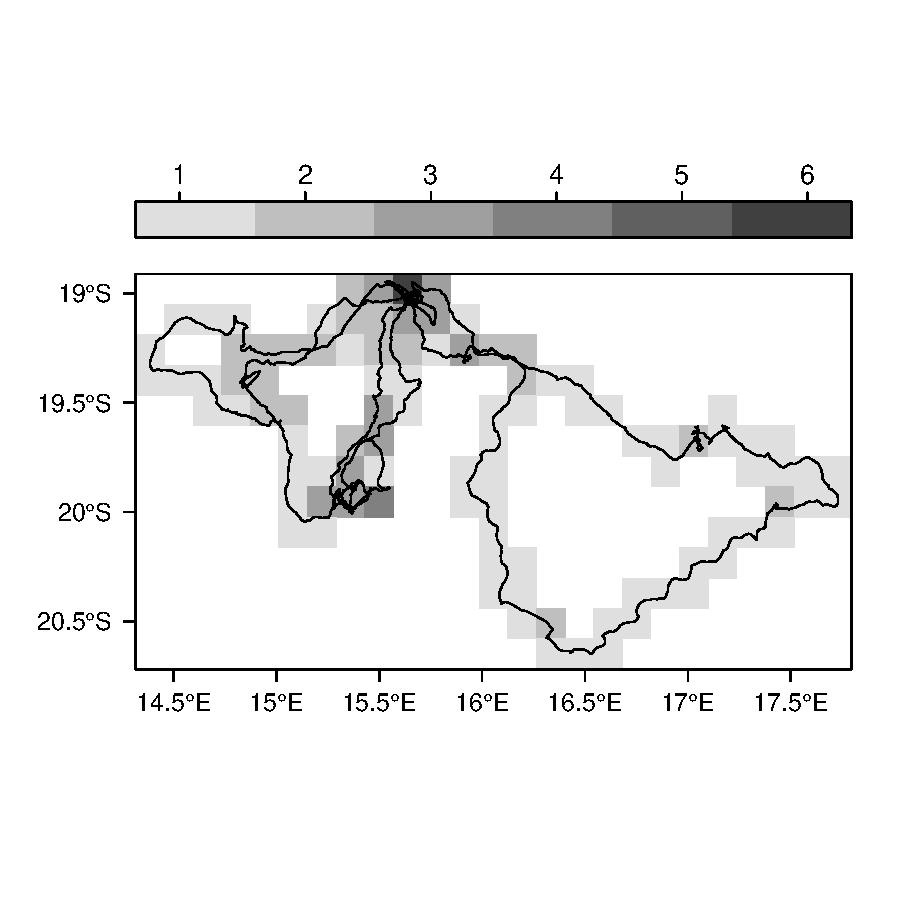
\includegraphics{trajagg-count_sp_vulture_TracksX1_fig_1}
\caption[Number of \code{Track} objects of a vulture counted over spatial geometries.]{Number of \code{Track} objects from the vulture individual X1 (\textit{Gyps africanus}) counted for each grid cell. The tracks (\code{Tracks\_X1}) are represented by \code{SpatialLines} and plotted above the \code{SpatialGrid}.}
\label{fig:counttracksx1oversp}
\end{figure}

\par\medskip

The following commands perform a count of tracks from the \code{TracksCollection} \code{vulture\_TrC} over a \code{SpatialGrid}, which covers the whole spatial extent of the first two \code{Tracks} objects from that \code{TracksCollection}. The argument \code{byID} is set to \code{TRUE} which results in separated counts for each individual.

\par\medskip

\begin{small}
\begin{Schunk}
\begin{Sinput}
> spG_X1X2_dim15 <- createSpatialArealObjFromPoints(
+   as(vulture_TrC[1:2], "SpatialPointsDataFrame"), 
+   desDim = 15, out = "SpatialGrid")
> count_vultureTrC_byID <- count(vulture_TrC, spG_X1X2_dim15, byID = TRUE)
> class(count_vultureTrC_byID)[1]
\end{Sinput}
\begin{Soutput}
[1] "SpatialGridDataFrame"
\end{Soutput}
\begin{Sinput}
> str(count_vultureTrC_byID@data)
\end{Sinput}
\begin{Soutput}
'data.frame':	135 obs. of  3 variables:
 $ ntraj_Tracks_X1: num  NA NA NA NA NA NA NA NA NA NA ...
 $ ntraj_Tracks_X2: num  NA NA NA 1 11 12 1 NA NA NA ...
 $ ntraj_Tracks_X3: num  NA NA NA NA NA NA 8 2 NA NA ...
\end{Soutput}
\end{Schunk}
\end{small}

\par\medskip

The \code{data} slot of the resulting \code{SpatialGridDataFrame} from the recent \code{count} call contains three attributes, each representing the number of \code{Track} objects per grid cell of one individual. The names of the attributes reflect the corresponding individuals respectively the \code{Tracks} objects of the corresponding individuals. The results are graphically shown in Figure \ref{fig:countvulturetrcbyidoversp}, whereas for a better design just the counts of the first two individuals are plotted.

\par\medskip

\begin{figure}[!htb]
\centering
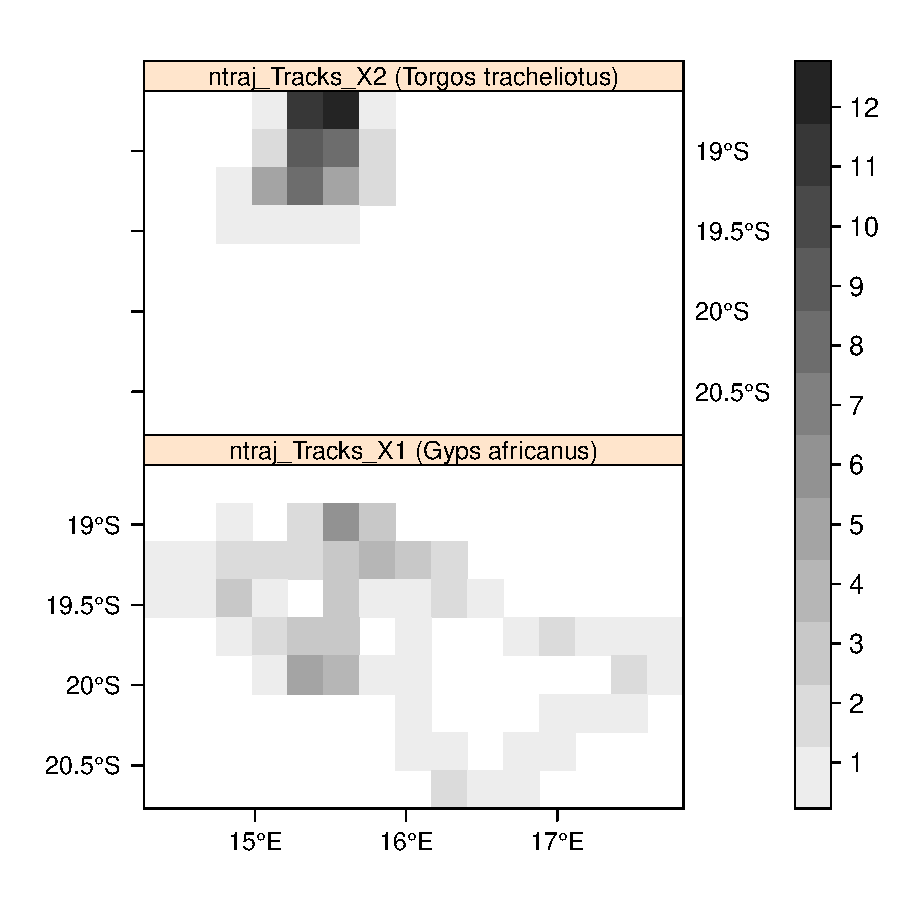
\includegraphics{trajagg-count_sp_vulture_TrC_fig_1}
\caption[Individual number of \code{Track} objects of two vultures counted over spatial geometries.]{Individual number of \code{Track} objects of two vulture individuals counted for each grid cell. Result from a call of \code{count} with a \code{TracksCollection} and \code{byID = TRUE}.}
\label{fig:countvulturetrcbyidoversp}
\end{figure}

\par\medskip

In the same way as the method \code{count} was applied in this subsection it  may also be applied with \code{by} arguments of class \code{STF}, which is presented in the Subsection~\ref{subsec:countoverstf}.

\par\medskip


% ----------------------------------------------------------------
\subsection{Counting trajectories over \codeintitles{STF} objects}
\label{subsec:countoverstf}

For \code{by} arguments of class \code{STF} the method \code{count} works analogous to the above presented functionality whereas the returned object is of class \code{STFDF}. For each spatio-temporal geometry the number of intersecting \code{Track} objects is counted. For illustration we need a \code{STF} object which may be passed to the \code{by} argument. Such an object  will be created by first creating an object of class \code{Spatial} as described above and then creating an object of class \code{STF} out of the \code{Spatial} object adding the desired temporal data to the slots \code{time} and (optional) \code{endTime}.
\par\medskip


The functionality of counting over a \code{STF} object will be presented on basis of the \code{Tracks} object \code{Tracks\_X3}.
With the following commands first an object of class \code{SpatialPixels} is created which covers the extent of the \code{Tracks} object \code{Tracks\_X3}. Subsequent a \code{STF} object is created out of the \code{SpatialPixels} containing four time intervals with an equal length of 3 days covering the first 12 of the 14 tracked days from \code{Tracks\_X3}. With the last command the method \code{count} is called with the \code{Tracks} object \code{Tracks\_X3} and the recently created \code{STF} object.

\par\medskip

\begin{small}
\begin{Schunk}
\begin{Sinput}
> spPix_X3_dim15 <- createSpatialArealObjFromPoints(
+   as(Tracks_X3, "SpatialPointsDataFrame"), 
+   desDim = 15, out = "SpatialPixels")
> stf_spPx_X3_4t <- STF(spPix_X3_dim15,
+                       time = Tracks_X3[c(1,4,7,10)]@tracksData$tmin,
+                       endTime = Tracks_X3[c(3,6,9,12)]@tracksData$tmax)
> count_Tracks_X3_stf <- count(Tracks_X3, stf_spPx_X3_4t)
\end{Sinput}
\end{Schunk}
\end{small}

\par\medskip

The result of the above call of \code{count} is presented in Figure \ref{fig:counttracksx3overstf}.
The Figure shows the number of \code{Track} entities from the \code{Tracks} object \code{Tracks\_X3} (\textit{Gyps africanus}) counted for each spatio-temporal geometry of the \code{STF} object built up out of \code{SpatialPixels} and four time intervals. Each of the four panels represents a three days time interval whose starting dates are given by the panel titles. One may identify some kind of a route with a north-south orientation which is passed by the vulture individual in three of the four time intervals on two tracks (\code{Track} objects). Due to the fact that one \code{Track} covers the vulture movement of one day we may interpret that the vulture passed that route at six of the twelve days of the total \code{STF} object time interval at least one time per day. At the both \textit{endpoints} of that north-south orientated route one may identify areas which were visited on two or three days of nearly each three day interval. Moreover one may identify some kind of day trips to the surrounding environment of that north-south orientated route especially during the first three time intervals.

\par\medskip

\begin{figure}[!htb]
\centering
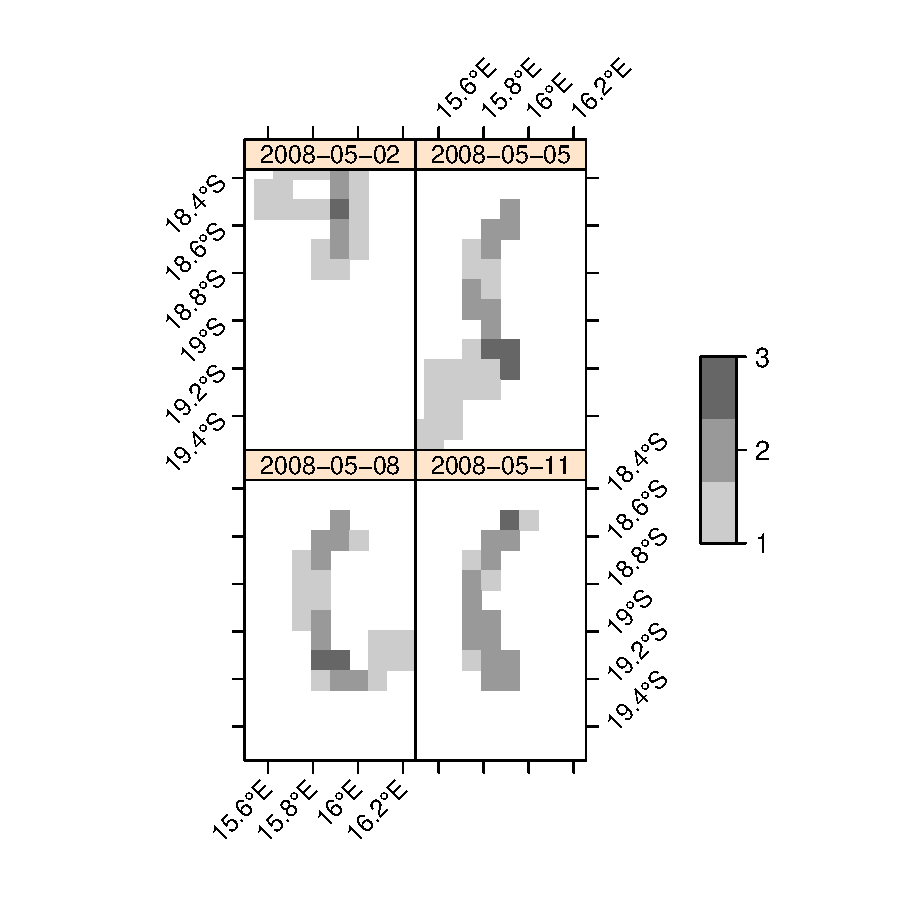
\includegraphics{trajagg-count_stf_vulture_X3_fig_1}
\caption[Number of \code{Track} objects of a vulture counted over spatio-temporal geometries.]{Number of \code{Track} objects of the vulture individual X3 (\textit{Gyps africanus}) counted over spatio-temporal geometries. Each panel represents a three days time interval whose starting dates are given by the panel titles.}
\label{fig:counttracksx3overstf}
\end{figure}


We see that with applying the method \code{count} one may retrieve basic information from trajectory data about the presence of one or more individuals related to spatial or spatio-temporal geometries. In the next Section (Section \ref{sec:aggreate}) the functionality of the method \code{aggregate} is presented which may be used to retrieve summary statistics of attribute data measured for \code{Track} point entities as well as to get further trajectory (meta-)data about the number of relocations and the approximate duration and distance corresponding to each spatio-temporal geometry.



%=====================================================================
% AGGREGATE
%---------------------------------------------------------------------
\section{\codeintitles{aggregate} - Aggregation of \pkg{trajectories} objects}
\label{sec:aggreate}

The aim of the implemented \code{aggregate} methods related to \pkg{trajectories} objects is to aggregate attribute values observed in conjunction with trajectory points' records on basis of a given grouping predicate, that is represented by spatial or spatio-temporal geometries.
An overview of the available S4 style \code{aggregate} methods for classes defined in \pkg{trajectories} could be obtained by the command \code{showMethods} again:
\par\medskip

\begin{small}
\begin{Schunk}
\begin{Sinput}
> showMethods(aggregate, classes = c("Track", "Tracks", "TracksCollection"))
\end{Sinput}
\begin{Soutput}
Function: aggregate (package stats)
x="Track"
x="Tracks"
x="TracksCollection"
\end{Soutput}
\end{Schunk}
\end{small}

Due to the facts that the \textit{original} \code{aggregate} method is a S3 style method (package \pkg{stats}) and that the implementation of \code{aggregate} in the package \pkg{trajaggr} uses internal methods to dispatch on the \code{by} argument, that represents the grouping predicate, the output of \code{showMethods} just shows the \code{x} argument of the \code{aggregate} methods. 
\par\medskip

The \code{aggregate} methods accept analogous to the methods \code{over} and \code{count} an  object inheriting from class \code{Spatial}, in particular a \code{SpatialPolygons}, \code{SpatialPixels} or \code{SpatialGrid} object, or a \code{STF} object as its grouping predicate.
The methods respect the spatial and temporal domain of the passed \code{trajectories} object which causes a consideration of the temporal domain even if a \code{Spatial} object is passed to the \code{by} argument. 
The returned object is always of class \code{STFDF}.
\par\medskip

Generally the implemented \code{aggregate} methods are geared to the \code{aggregate} methods implemented in \pkg{sp} and \pkg{spacetime} related to the arguments, that may be specified.
Arguments known from the mentioned methods are \code{x} for the object whose data should be aggregated, \code{by} for the grouping predicate, \code{FUN} for the aggregation function and \code{simplify}.
If \code{simplify} is specified as \code{TRUE} (default) it affects the return of the \code{aggregate} methods if the dimension of the temporal or spatial domain of the grouping predicate equals one.
In such cases the returned object is \textit{simplified} by dropping the domain whose dimension equals one and in case of aggregation of \pkg{trajectories} objects the returned \textit{simplified} objects may be of class \code{Spatial}, if the temporal domain is dropped, or of class \code{xts}, if the spatial domain is dropped.
\par\medskip

Besides these arguments mentioned above the \code{aggregate} methods for \code{trajectories} objects are using further arguments depending of the class of the object passed to the \code{x} argument. In particular these further arguments are \code{use.data}, \code{weight.points}, \code{weight.tracks} and \code{byID} which are introduced in detail in Section \ref{sec:generalaspects}.
\par\medskip

In cases where \code{x} is of class \code{Tracks} or \code{TracksCollection} the \code{data} slots of the \code{Track} objects are checked for consistency related to the existence of attributes by comparing the \code{data.frame} column \code{names}. This is performed because it is not a requirement related to the classes defined in \pkg{trajectories}, that all \code{Track} objects' \code{data} slots are \textit{identical}.
In the case of disparity of the \code{data} slots missing columns are added to the relevant \code{data.frame} objects and filled with \code{NA} values. 
But note that if \code{aggregate} is called with a \code{TracksCollection} and \code{byID = TRUE} this consistency check of the \code{data.frame} objects is just performed individually for each \code{Tracks} object, and it is not ensured that the different \code{Tracks} objects have \textit{identical} \code{data} slots.
\par\medskip

Spatio-temporal aggregation of \pkg{trajectories} objects over \code{STF} objects is illustrated in Subsection \ref{subsec:aggoverstf} by applying the \code{aggregation} method to the \pkg{trajectories} objects coerced from the \code{vulture\_moveStack} example data.
The Subsection \ref{subsec:aggregationbysp} the aggregation with a \code{Spatial} grouping predicate applied to \pkg{trajectories} objects coerced from the pigeons' example data is presented.
\par\medskip




%=====================================================================
% AGGREGATE SPATIO-TEMPORAL
%---------------------------------------------------------------------
\subsection{Spatio-temporal aggregation of \pkg{trajectories} objects}
\label{subsec:aggoverstf}

The spatio-temporal aggregation of \pkg{trajectories} objects over an object of class \code{STF} performed by the method \code{aggregate} returns an objects of class \code{STFDF} with the same spatial and temporal component as the passed grouping predicate.
The \code{STFDF} object's \code{data} slot contains the aggregated attribute values corresponding to each particular spatio-temporal geometry of the grouping predicate.
\par\medskip

As mentioned in the introduction of this chapter the \pkg{trajectories} objects coerced from the \code{vulture\_moveStack} example data are used to illustrate the aggregation.
Before the \code{vulture\_moveStack} object may be coerced to suitable structured \code{Tracks} and \code{TracksCollection} objects some preparation is needed which is motivated and illustrated in conjunction with the coercion in Appendix \ref{sec:prepvulturemovestackforcount}.
\par\medskip

As an first example we will calculate the minimal altitude of a vulture individual (\textit{Gyps africanus}) over spatio-temporal regions. Due to the aggregation function calculating the minimum in conjunction with the selected attribute representing the altitude there is neither the need nor the option of using a weighted aggregation approach to obtain a meaningful aggregation result.
\par\medskip

By the following commands first a \code{STF} is created. That object has a \code{sp} slot with \code{SpatialPixels} covering the spatial extent of the \code{Tracks} object \code{Tracks\_X1}, that represents 14~day-tracks of a vulture individual. 
Related to the time domain the \code{STF} object has four time intervals each covering three days of the 14~days the vulture was tracked. 
Subsequently the attribute \code{height\_raw} of the \code{Tracks\_X1} object, selected by the argument \code{use.data}, is (unweighted) aggregated over the spatio-temporal geometries of the created \code{STF} object.
As aggregation function the function \code{min} is passed to the argument \code{FUN}, which determines the  minimal altitude of the vulture individual for each spatio-temporal geometry. 
\par\medskip

\begin{small}
\begin{Schunk}
\begin{Sinput}
> # Create SpatialPixels covering the extent of the Tracks_X1 object
> spPix_X1_dim15 <- createSpatialArealObjFromPoints(
+   as(Tracks_X1, "SpatialPointsDataFrame"), 
+   desDim = 15, out = "SpatialPixels")
> # Create a STF object with four time intervals
> stf_px_X1_4t <- STF(spPix_X1_dim15,
+                     time = Tracks_X1[c(1,4,7,10)]@tracksData$tmin,
+                     endTime = Tracks_X1[c(3,6,9,12)]@tracksData$tmax)
> # Aggregate the attribute 'height_raw' using function 'min'
> agg_X1_stf_minHght <- aggregate(x = Tracks_X1, by = stf_px_X1_4t, FUN = min,
+                                 na.rm = TRUE, use.data = "height_raw")
> # Class of returned object
> class(agg_X1_stf_minHght)[1]
\end{Sinput}
\begin{Soutput}
[1] "STFDF"
\end{Soutput}
\begin{Sinput}
> # Some example rows from the data slot of the resulting STFDF object
> agg_X1_stf_minHght@data[474:477, ]
\end{Sinput}
\begin{Soutput}
    height_raw nlocs approx_duration approx_distance ntraj
474        8.6    68         17343.0        13314.09     1
475       22.5    43          7440.0        37409.59     1
476      707.5     2           240.5         3480.54     1
477         NA    NA              NA              NA    NA
\end{Soutput}
\end{Schunk}
\end{small}

\par\medskip

The output shows that the object returned from the method \code{aggregate} is of class \code{STFDF} and that the \code{data} slot of the returned \code{STFDF} object contains the aggregated values of the selected attribute \code{height\_raw} as well as the calculated metadata for each spatio-temporal geometry. 
The metadata is being composed of the variables \code{nlocs}, representing the number of trajectory points, \code{approx\_duration}, representing the overall sum of duration assigned to the trajectory points, \code{approx\_distance}, representing the overall sum of distance assigned to the trajectory points, and \code{ntraj}, representing the number of trajectories intersecting the particular geometries. 
\par\medskip

The Figure \ref{fig:aggtracksx1overstf} gives a visual representation of the aggregated values of the attribute \code{height\_raw} indicating the minimal altitude of the vulture for each spatio-temporal geometry. The graphic is divided into four panels each representing a three days time interval, whose starting date is indicated by the panel title.
From the figure one may for instance derive the information in which spatio-temporal regions the vulture individual stayed on the one hand at least temporarily on or near to the ground and on the other hand which regions were overflown with an enormous altitude.
\par\medskip


\begin{figure}[!htb]
\centering
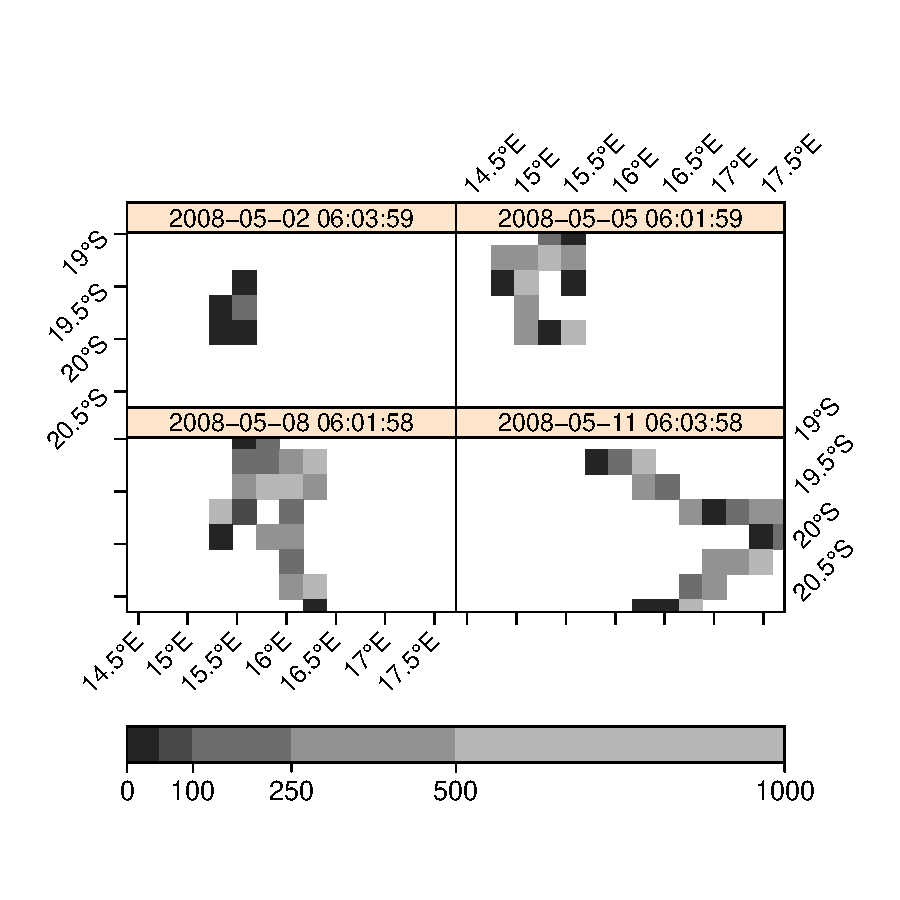
\includegraphics{trajagg-agg_stf_vulture_Tracks_X1_fig_1}
\caption[Minimal altitude of a vulture obtained by aggregation over spatio-temporal geometries.]{Minimal altitude of the vulture individual X1 (\textit{Gyps africanus}) over spatial regions and four consecutive 3-days time intervals. Result from the method \code{aggregate} applied to a \code{Tracks} object and a spatio-temporal grouping predicate. Each panel represents one of the 3-days time intervals whose starting dates are given by the panel titles. The altitude is given in metres.}
\label{fig:aggtracksx1overstf}
\end{figure}


In the following example the individual average speed of three vulture individuals, whose trajectories are stored in an object of class \code{TracksCollection}, over spatio-temporal regions is calculated.
Due to the temporal reference of the attribute speed in conjunction with the aim to calculate averaged values a aggregation weighted by time is suitable. 
In particular this includes a weighted aggregation of the measurements corresponding to the trajectory points for each \code{Track} due to a slightly irregular sampling rate as well as a weighted aggregation of the aggregated values corresponding to each \code{Track} due to the temporal reference of the attribute speed.
\par\medskip

The described approach of the aggregation of the vultures' speed is realized by the commands following further down.
For the grouping predicate the \code{STF} object from the last \code{aggregate} call is used, which in fact does not cover the whole spatial extent of the \code{TracksCollection}, but for visual presentation of the aggregation results just the aggregated values of the first individual (\code{Tracks\_X1}) will be plotted.
\par\medskip

To realize the weighted aggregation of the \code{TracksCollection} object \code{vulture\_TrC}, which is created by coercion from the \code{vulture\_moveStack} (Appendix \ref{sec:prepvulturemovestackforcount}), a weighted aggregation function needs to be passed to the argument \code{FUN} and further arguments need to be specified.
The function \code{weighted.mean} is passed to the \code{FUN} argument, and the \code{character} string 'byTime' is passed to the arguments \code{weight.points} and \code{weight.tracks} to indicate that the used weights should be based on the duration assigned to the \code{Track} points and \code{Track} \textit{parts}
intersecting the particular spatio-temporal geometries as described in Section \ref{sec:meaningfulrealization}. 
Moreover the argument \code{byID} is set to \code{TRUE} to indicate that the aggregated values are calculated individually for each vulture respectively for each \code{Tracks} object.
By the way an aggregation of a \code{TracksCollection} with calculating aggregated values over all \code{Tracks} objects (\code{byID = FALSE}) is performed in Subsection \ref{subsec:aggregationbysp}.
\par\medskip

The ability of creating missing attribute columns in particular \code{Track} objects in cases where the \code{data} slots of the \code{Track} objects for instance of a \code{Tracks} object are inconsistent related to the existing columns is described in the introduction of this section.
To illustrate that ability the attribute \code{ground\_speed} is delete from 13 of the 14 \code{Track} objects from the second vulture individual respectively from the second \code{Tracks} object of the \code{TracksCollection}, as one may realize from the following commands.
\par\medskip

\begin{small}
\begin{Schunk}
\begin{Sinput}
> # Identify the index of the attribute ground_speed
> w_spd <- which(names(vulture_TrC[2][2]@data) == "ground_speed")
> # To illustrate the creation of missing attributes the attribute
> # ground_speed is deleted from the data of the second vulture
> for (i in 2:length(vulture_TrC@tracksCollection[[2]]@tracks)) {
+   vulture_TrC@tracksCollection[[2]]@tracks[[i]]@data <- 
+     vulture_TrC@tracksCollection[[2]]@tracks[[i]]@data[ , -w_spd]
+ }
> # Attribute still available in e.g. second Track...?
> "ground_speed" %in% names(vulture_TrC[2][2]@data)
\end{Sinput}
\begin{Soutput}
[1] FALSE
\end{Soutput}
\begin{Sinput}
> # Weighted aggregation of the TracksCollection separated by individuals
> agg_vTrC_wMeanSpd <- aggregate(x = vulture_TrC, by = stf_px_X1_4t,
+                                FUN = weighted.mean, na.rm = TRUE, 
+                                use.data = "ground_speed",
+                                weight.points = "byTime", 
+                                weight.tracks = "byTime", byID = TRUE)
> # Overview of individual ground_speed
> summary(agg_vTrC_wMeanSpd@data[["Tracks_X1.ground_speed"]])
\end{Sinput}
\begin{Soutput}
   Min. 1st Qu.  Median    Mean 3rd Qu.    Max.    NA's 
  1.108   6.703  15.200  12.560  16.370  22.430     422 
\end{Soutput}
\begin{Sinput}
> summary(agg_vTrC_wMeanSpd@data[["Tracks_X2.ground_speed"]])
\end{Sinput}
\begin{Soutput}
   Min. 1st Qu.  Median    Mean 3rd Qu.    Max.    NA's 
  1.700   2.519   3.339   3.339   4.158   4.977     478 
\end{Soutput}
\begin{Sinput}
> summary(agg_vTrC_wMeanSpd@data[["Tracks_X3.ground_speed"]])
\end{Sinput}
\begin{Soutput}
   Min. 1st Qu.  Median    Mean 3rd Qu.    Max.    NA's 
 0.5988  2.8910  8.4630  8.4710 13.4300 15.4700     467 
\end{Soutput}
\end{Schunk}
\end{small}

\par\medskip

The output of the above commands shows that it is no problem related to the aggregation process if some attributes are missing in some \code{Track} objects of a \code{Tracks}. 
The aggregated values of \code{ground\_speed} of the second \code{Tracks} object (\code{Tracks\_X2.ground\_speed}) returned by the \code{summary} command are relatively small compared to the other \code{Tracks} objects' aggregated values.
This is explained by the deletion of the speed attribute values of 13 of the 14 \code{Track} objects of the second \code{Tracks} object, even if that is not directly proved by the above commands.
\par\medskip

The Figure \ref{fig:aggtrackscolloverstf} visually presents the aggregated values of \code{ground\_speed} indicating the weighted averaged speed of the vulture individual for each spatio-temporal geometry. The graphic is again divided into four panels each representing a three days time interval, whose starting date is indicated by the panel title.
From the figure one may derive the information in which spatio-temporal regions the vulture individual was moving fast which may indicate (continuous) flying over long periods.
For spatio-temporal regions where the averaged speed is lower one may derive that the vulture at least stayed a certain time on the ground or its movement was characterized by an alternation of flying (shorter distances) and continuing at a certain position.
\par\medskip

\begin{figure}[!htb]
\centering
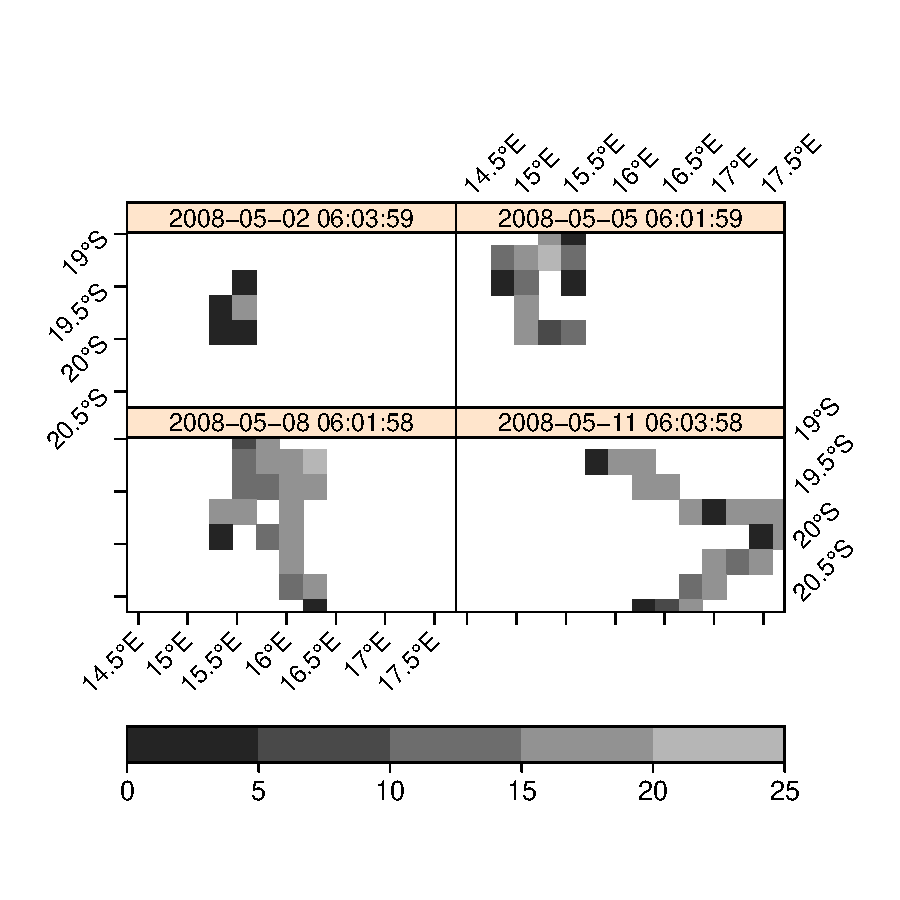
\includegraphics{trajagg-agg_stf_vulture_TrC_fig_2}
\caption[Weighted average speed of a vulture obtained by aggregation over spatio-temporal geometries.]{Weighted average speed of the vulture individual X1 (\textit{Gyps africanus}) over spatial regions and four consecutive 3-days time intervals. Result from the method \code{aggregate} applied to a \code{TracksCollection} object and a spatio-temporal grouping predicate in conjunction with \code{byID = TRUE}. Each panel represents one of the 3-days time intervals whose starting dates are given by the panel titles. The speed is given in metres per second.}
\label{fig:aggtrackscolloverstf}
\end{figure}


One may also easily compare Figure \ref{fig:aggtracksx1overstf} and Figure \ref{fig:aggtrackscolloverstf} due to the identical grouping predicate that was used in the \code{aggregate} calls.
There is a relation between the minimal altitude of the vulture (Figure \ref{fig:aggtracksx1overstf}) and the weighted averaged speed (Figure~\ref{fig:aggtrackscolloverstf}), especially in the extremely low values of altitude and speed, as one also would expect. 
\par\medskip

In the following Subsection \ref{subsec:aggregationbysp} the method \code{aggregate} for \pkg{trajectories} objects with a grouping predicate of class \code{Spatial} passed to the \code{by} argument is presented, and for its illustration the pigeon example data sets introduced in Section \ref{sec:exampledatamovebank} are used.
\par\medskip



%=====================================================================
% AGGREGATE SPATIAL
%---------------------------------------------------------------------
\subsection{Spatial aggregation of \pkg{trajectories} objects}
\label{subsec:aggregationbysp}

This subsection presents the meaningful aggregation of trajectory objects defined in the package \pkg{trajectories} over a \code{Spatial} grouping predicate. If the method \code{aggregate} is applied with a \code{Spatial} grouping predicate the returned object is of class \code{STFDF}, that is characterized by a \code{sp} slot containing an object equivalent to the grouping predicate. The temporal information of the \code{STFDF} object is characterized by time instances, that are derived from the unique timestamps of those trajectory points, that are spatially intersecting the geometries of the grouping predicate. This approach respects and preserves the temporal information of the trajectories related to the returned aggregation result.
\par\medskip

For illustration of the aggregation the pigeons example data sets, introduced in Section \ref{sec:exampledatamovebank}, are used. In particular these are two \code{MoveStack} objects each containing two (subsets of) trajectories of a pigeon individual. In each case the trajectories of the different individuals are sampled synchronously and their sampling rates are characterized by a high frequency with four samples per second. 
Due to the aggregation approach the call of \code{aggregate} with a \code{Spatial} object passed to the \code{by} argument needs a huge amount of computation time. To avoid that in the following example a minimal subset of the pigeons example data and a \code{Spatial} object with just a few geometries are created and passed to the \code{aggregate} method.
\par\medskip

The \code{MoveStack} objects \code{pigeon\_R\_moveSt\_sub} and \code{pigeon\_S\_moveSt\_sub}, which represent the minimal subsets of the pigeon example data sets, are coerced to \code{Tracks} objects. Afterwards in each case the \code{Tracks} are reduced to a subset containing just the first \code{Track} object and these reduced \code{Tracks} objects are combined to a \code{TracksCollection} object, which is shown and validated by the following commands.
\par\medskip

\begin{small}
\begin{Schunk}
\begin{Sinput}
> # Load the small subsets of the example data sets
> data(pigeon_R_moveSt_sub, pigeon_S_moveSt_sub)
> # Validate the class
> is(pigeon_R_moveSt_sub, "MoveStack") || is(pigeon_S_moveSt_sub, "MoveStack")
\end{Sinput}
\begin{Soutput}
[1] TRUE
\end{Soutput}
\begin{Sinput}
> # Coerce MoveStacks to Tracks objects and validate the returned object
> pigeon_R_Tr <- as.Tracks(pigeon_R_moveSt_sub)
> pigeon_S_Tr <- as.Tracks(pigeon_S_moveSt_sub)
> is(pigeon_R_Tr, "Tracks") || is(pigeon_S_Tr, "Tracks")
\end{Sinput}
\begin{Soutput}
[1] TRUE
\end{Soutput}
\begin{Sinput}
> # Inspect the high frequent and synchronious sampling rate
> options(digits.secs=2)
> index(pigeon_R_Tr[1]@time[1:5])
\end{Sinput}
\begin{Soutput}
[1] "2012-06-19 11:36:56.00 UTC"
[2] "2012-06-19 11:36:56.25 UTC"
[3] "2012-06-19 11:36:56.50 UTC"
[4] "2012-06-19 11:36:56.75 UTC"
[5] "2012-06-19 11:36:57.00 UTC"
\end{Soutput}
\begin{Sinput}
> options(digits.secs=0)
> length(pigeon_R_Tr[1]@time)
\end{Sinput}
\begin{Soutput}
[1] 60
\end{Soutput}
\begin{Sinput}
> identical(index(pigeon_R_Tr[1]@time), index(pigeon_S_Tr[1]@time))
\end{Sinput}
\begin{Soutput}
[1] TRUE
\end{Soutput}
\begin{Sinput}
> # Create a TracksCollection with one Track object od each individual
> pigeons_TrColl <- TracksCollection(
+   list(Tracks(list(pigeon_R_Tr[1])), Tracks(list(pigeon_S_Tr[1]))))
> # Inspect the tracksCollectionData
> pigeons_TrColl@tracksCollectionData[ , -c(6, 7)]
\end{Sinput}
\begin{Soutput}
        n     xmin     xmax     ymin     ymax
Tracks1 1 8.936704 8.939813 47.52063 47.52178
Tracks2 1 8.936752 8.939868 47.52062 47.52177
\end{Soutput}
\end{Schunk}
\end{small}

The output validates the statements from the two paragraphs above especially about the high frequent and synchronous sampling rates and shows that both \code{Track} objects from the \code{TracksCollection} contain 60 geometries respectively (measurement) points.
\par\medskip

It is important to know, that the trajectories of the two pigeon individuals are following almost the same course, which may be explained due to the fact that the trajectory data comes from a project, that studied the leadership-based flock structures of homing pigeons. The \code{tracksCollectionData} confirms that due to almost similar minimal and maximal x and y coordinates of the two \code{Tracks} objects.
\par\medskip

As an example for the method \code{aggregate} with a \code{Spatial} object passed to the \code{by}  argument of the \code{aggregate} method the attribute \code{ground\_speed} from the pigeons' trajectories is aggregated by the commands further down using \code{weighted.mean} as the aggregation function that is passed to the argument \code{FUN}. 
Due to the regular sampling rate there is no need to weight the particular \code{Track} point measurements, but due to the temporal reference of the attribute \code{ground\_speed} weighting of the particular \code{Track} object \textit{parts}, that intersect a particular spatial geometry of the grouping predicate, according to the assigned duration, is appropriate. For details about the assignment of duration to \code{Track} points and \textit{parts} see Section \ref{sec:meaningfulrealization}. Consequential the arguments related to the weighting process are specified as \code{weight.points = "equal"} to prevent the weighting of \code{Track} point measurements and \code{weight.tracks = "byTime"} to enable the weighting of \code{Track} \textit{parts} according to their assigned duration.
\par\medskip

By the following commands a \code{Spatial} object covering the whole spatial extent of the \code{TracksCollection} \code{pigeons\_TrColl} is created using a simple provided function that is introduced in Chapter \ref{chap:exampledata}. Afterwards the attribute \code{ground\_speed} is aggregated over this \code{Spatial} object as described in the previous paragraph.
\par\medskip

\begin{small}
\begin{Schunk}
\begin{Sinput}
> # Create SpatialPixels covering the extent of the TracksCollection
> spPix_pTrC_dim4 <- createSpatialArealObjFromPoints(
+   as(pigeons_TrColl, "SpatialPointsDataFrame"), 
+   desDim = 4, out = "SpatialPixels")
> # Dimensions of the SpatialPixels
> spPix_pTrC_dim4@grid@cells.dim
\end{Sinput}
\begin{Soutput}
[1] 4 2
\end{Soutput}
\begin{Sinput}
> # Aggregate the attribute 'ground_speed' using function 'weighted.mean'
> agg_pTrC_sp_wMeanSpd <- aggregate(x = pigeons_TrColl, by = spPix_pTrC_dim4,
+                                   FUN = weighted.mean, na.rm = TRUE,
+                                   use.data = "ground_speed",
+                                   weight.points = "equal", 
+                                   weight.tracks = "byTime", byID = FALSE)
> # Class of returned object
> class(agg_pTrC_sp_wMeanSpd)[1]
\end{Sinput}
\begin{Soutput}
[1] "STFDF"
\end{Soutput}
\begin{Sinput}
> # Dimensions of the returned STFDF object
> dim(agg_pTrC_sp_wMeanSpd)
\end{Sinput}
\begin{Soutput}
    space      time variables 
        8        60         5 
\end{Soutput}
\begin{Sinput}
> # Summary and example rows of the data slot of the resulting STFDF object
> summary(agg_pTrC_sp_wMeanSpd@data[ , -c(3, 4)])
\end{Sinput}
\begin{Soutput}
  ground_speed       nlocs           ntraj      
 Min.   :17.65   Min.   :1.000   Min.   :1.000  
 1st Qu.:18.65   1st Qu.:2.000   1st Qu.:2.000  
 Median :18.96   Median :2.000   Median :2.000  
 Mean   :19.00   Mean   :1.967   Mean   :1.967  
 3rd Qu.:19.33   3rd Qu.:2.000   3rd Qu.:2.000  
 Max.   :19.98   Max.   :2.000   Max.   :2.000  
 NA's   :419     NA's   :419     NA's   :419    
\end{Soutput}
\begin{Sinput}
> agg_pTrC_sp_wMeanSpd@data[c(209:212, 217:219), -4]
\end{Sinput}
\begin{Soutput}
    ground_speed nlocs approx_duration ntraj
209           NA    NA              NA    NA
210     19.93889     1            0.25     1
211     18.70833     1            0.25     1
212           NA    NA              NA    NA
217           NA    NA              NA    NA
218     19.17917     2            0.50     2
219           NA    NA              NA    NA
\end{Soutput}
\end{Schunk}
\end{small}

The output of the commands above shows that the dimensions of the returned \code{STFDF} object correspond to the spatial dimensions of the spatial grouping predicate in conjunction with the (unique) temporal dimensions respectively timestamps of the \code{pigeons\_TrColl} representing the synchronous sampling rate. The number of the synchronous timestamps was shown in the last but one block of \proglang{R} commands.
\par\medskip

To further interpret the output of the \proglang{R} commands it is useful to remember, that the trajectories of the two pigeons are following almost the same course. Thus two synchronously sampled \code{Track} points mostly intersect the same spatial geometry of the grouping predicate.
\par\medskip

The output of the \code{summary} command and the subset of the \code{data} slot show that the majority of the spatio-temporal geometries which at least correspond to one \code{Track} point (thus those geometries whose values are not \code{NA}) have two corresponding \code{Track} points, one of each \code{Tracks} object.
Cases in which just one \code{Track} point corresponds to a spatio-temporal geometry indicate that the temporally corresponding \code{Track} point from the other \code{Tracks} object intersects another geometry of the spatial grouping predicate. 
In such rare cases this second \code{Track} point intersects in the result of this particular aggregation (mostly) a \textit{neighbouring} spatial geometry of the grouping predicate. 
This is indicated by the two consecutive rows of the subset of the \code{data} slot, that both correspond to one \code{Track} point. The rows 210 and 218 correspond to the same spatial geometry of the grouping predicate due to its \code{length}, which is eight. 
Thus the row 211 corresponds to a \textit{neighbouring} geometry of the geometry corresponding to row 210 due to the fact that spatial features are cycled before proceeding in the temporal domain.
\par\medskip

In Figure \ref{fig:aggpigeonsoversp} the aggregation results are visually presented by time series of the weighted average speed individually for each spatial geometry of the grouping predicate. 
\par\medskip

\begin{figure}[!htb]
\centering
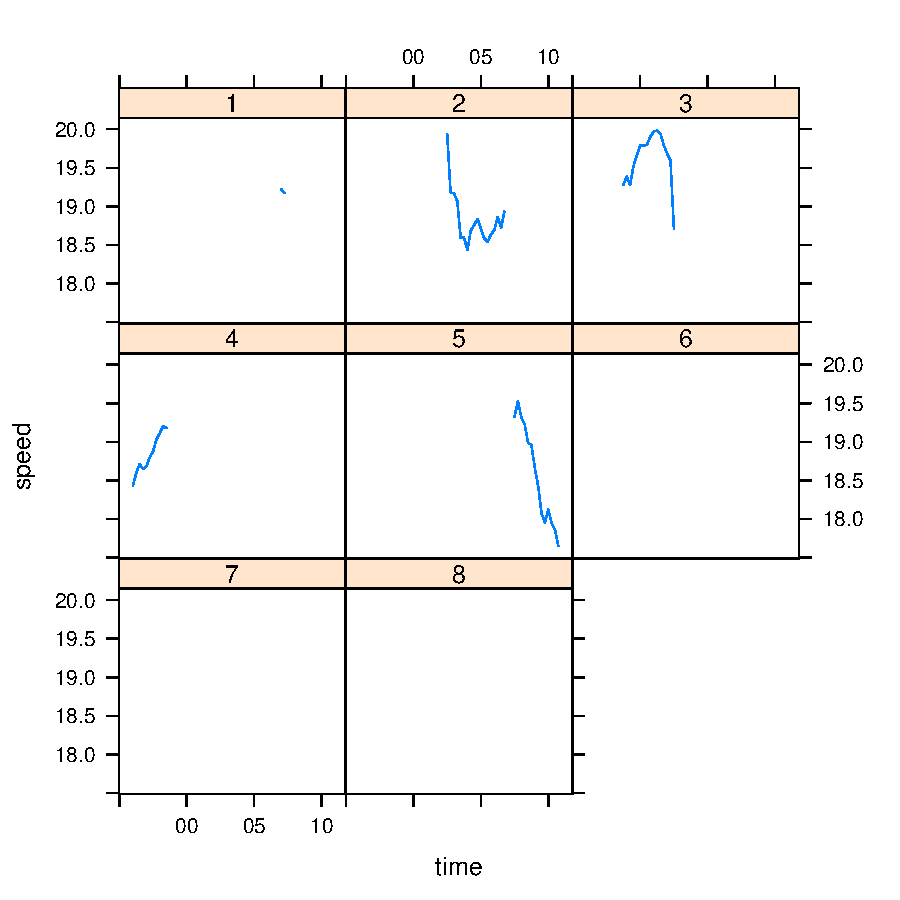
\includegraphics{trajagg-agg_sp_pigeon_TrColl_fig_1}
\caption[Time series of aggregated speed values from two pigeons separated by spatial geometries.]{Time series of aggregated speed values from two synchronously and regularly sampled trajectories of two pigeon individuals (\textit{Columba livia}) flying along the same course. The time series are separated for each spatial region of the spatial grouping predicate used for the weighted aggregation.}
\label{fig:aggpigeonsoversp}
\end{figure}


In the following subsection the ability of performing a spatial aggregation of \pkg{trajectories} objects without respecting the temporal information of these objects is shortly introduced and illustrated. The aggregation is performed using the pigeons example data sets which may further help to clarify its characteristics.


\subsection{Spatial aggregation of \pkg{trajectories} objects ignoring time}
\label{subsec:aggregationbyspigntime}

Results of a \textit{pure} spatial aggregation ignoring and loosing the temporal information of the trajectory data may be obtained by applying the \code{aggregate} method described in Section \ref{subsec:aggoverstf} with a \code{STF} object containing just one time interval which covers the whole duration of the \pkg{trajectories} object of interest.
\par\medskip

With the further down following commands such an aggregation is performed using in each case the second trajectory of the example data sets \code{pigeon\_R\_moveStack} and \code{pigeon\_S\_moveStack}. The characteristics of these trajectories are similar to those used for aggregation in Subsection \ref{subsec:aggregationbysp}. For further details about the example data sets call for instance \code{?pigeon\_R\_moveStack} or see Section \ref{sec:exampledatamovebank}. 
\par\medskip

In this approach we are aggregating the attribute \code{ground\_speed} again using the weighted aggregation function \code{weighted.mean}, and thus the arguments \code{weight.points} and \code{weight.tracks} are set in the same manner as in the call of the method \code{aggregate} in Subsection \ref{subsec:aggregationbysp}.
But this time the argument \code{simplify} needs to be \code{TRUE}, so that the returned object, that is normally of class \code{STFDF} may be \textit{simplified} to an object equivalent to the \code{sp} slot of the \code{STF} object passed to the argument \code{by}. Indeed the argument \code{simplify} is \code{TRUE} by default, but its importance in this context needs to be mentioned and it is explicitly set in the method call to clarify this importance.
\par\medskip

Before we may call the method \code{aggregate} we need to coerce the \code{MoveStack} objects to \code{Tracks} objects, whose second \code{Track} objects are combined to a \code{TracksCollection} afterwards. Moreover we have to create an adequate \code{STF} object with one time interval covering the whole duration of all \code{Track} objects which are part of the \code{TracksCollection}. All that including the aggregation and the inspection of the result is done by the following commands.


\begin{small}
\begin{Schunk}
\begin{Sinput}
> # Load data
> data(pigeon_R_moveStack, pigeon_S_moveStack)
> # Coerce to Tracks
> pigeon_R_Trcs <- as.Tracks(pigeon_R_moveStack)
> pigeon_S_Trcs <- as.Tracks(pigeon_S_moveStack)
> # Create a TracksCollection
> pigeons_TrC <- TracksCollection(list(Tracks(list(pigeon_R_Trcs[2])),
+                                      Tracks(list(pigeon_S_Trcs[2]))))
> # Create SpatialPixels covering the extent of the TracksCollection
> spPix_pTrC_dim15 <- createSpatialArealObjFromPoints(
+   as(pigeons_TrC, "SpatialPointsDataFrame"), 
+   desDim = 15, out = "SpatialPixels")
> # Create a STF object with one overall time interval
> # Note: currently time zone problem in tracksCollectionData with V. 0.1-1
> #stf_px_pTrC_1t <- STF(spPix_pTrC_dim15,
> #                      time = pigeons_TrC@tracksCollectionData$tmin[1],
> #                      endTime = pigeons_TrC@tracksCollectionData$tmax[1])
> stf_px_pTrC_1t <- STF(spPix_pTrC_dim15,
+                       time = pigeon_R_Trcs@tracksData$tmin[2],
+                       endTime = pigeon_R_Trcs@tracksData$tmax[2])
> # Aggregate the attribute 'height_raw' with FUN = weighted.mean
> agg_pTrC_wMeanSpd <- aggregate(x = pigeons_TrC, by = stf_px_pTrC_1t, 
+                                FUN = weighted.mean, na.rm = TRUE,
+                                use.data = "ground_speed",
+                                simplify = TRUE, weight.points = "equal", 
+                                weight.tracks = "byTime", byID = FALSE)
> class(agg_pTrC_wMeanSpd)[1]
\end{Sinput}
\begin{Soutput}
[1] "SpatialPixelsDataFrame"
\end{Soutput}
\begin{Sinput}
> summary(agg_pTrC_wMeanSpd@data[c(1, 2, 5)])
\end{Sinput}
\begin{Soutput}
  ground_speed       nlocs            ntraj     
 Min.   :14.57   Min.   :  2.00   Min.   :1.00  
 1st Qu.:15.83   1st Qu.: 23.00   1st Qu.:2.00  
 Median :17.64   Median : 39.00   Median :2.00  
 Mean   :17.24   Mean   : 38.32   Mean   :1.92  
 3rd Qu.:18.17   3rd Qu.: 46.00   3rd Qu.:2.00  
 Max.   :19.46   Max.   :108.00   Max.   :2.00  
 NA's   :80      NA's   :80       NA's   :80    
\end{Soutput}
\end{Schunk}
\end{small}


The output shows that the returned object is of class \code{SpatialPixelsDataFrame} and thus the object representing the aggregation result is \textit{simplified}, because typically an object of class \code{STFDF} is returned.
\par\medskip

Moreover the \code{summary} command gives an overview of the aggregated speed values (\code{ground\_speed}) as well as of the number of trajectory points (\code{nlocs}) and the number of \code{Track} objects (\code{ntraj}), that is determined by the presence of \code{Track} points, for each spatial geometry of the \code{SpatialPixelsDataFrame}. 
The attribute \code{ntraj} shows that the majority of the spatial geometries, that are intersected by at least one \code{Track} point, are intersected by both \code{Tracks} objects, which confirms the statement from the Subsection~\ref{subsec:aggregationbysp}, that the pigeons are flying along the same course.
\par\medskip

A visual presentation of the aggregation result is given by Figure \ref{fig:aggoverspaceigntime}. The figure shows the weighted average speed values in metres per second of the two pigeon individuals for each spatial geometry of the grouping predicate.
\par\medskip

\begin{figure}[!htb]
\centering
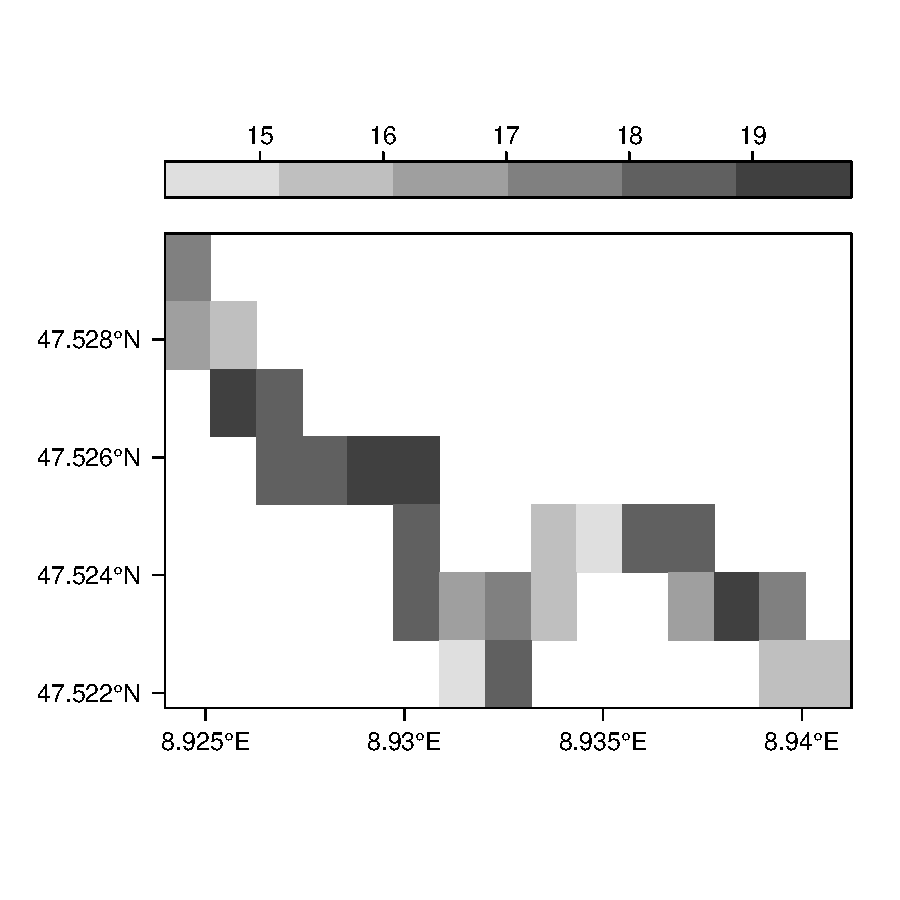
\includegraphics{trajagg-agg_stf_pureSpatial_fig_1}
\caption[Weighted average speed of two pigeons obtained by aggregation over a \code{Spatial} grouping predicate with no respect of time]{Weighted average speed of two pigeon individuals (\textit{Columba livia}) obtained by weighted aggregation over a \code{Spatial} grouping predicate with no respect of the temporal characteristics of the trajectories. Speed is given in metres per second.}
\label{fig:aggoverspaceigntime}
\end{figure}





%%%%%%%%%%%%%%%%%%%%%%%%%%%%%%%%%%%%%%%%%%%%%%%%%%%%%%%%%%%%%%%%%%
%%% Discussion %%%
%%%%%%%%%%%%%%%%%%%%%%%%%%%%%%%%%%%%%%%%%%%%%%%%%%%%%%%%%%%%%%%%%%

\chapter{Discussion}
\label{chap:discussion}

In this chapter the strengths and weaknesses of the implemented methods are discussed.
In general meaningful methods for spatial and spatio-temporal overlay of \code{Track} objects and for spatial and spatio-temporal aggregation of objects of all classes for trajectories that are defined in the package \pkg{trajectories} are implemented. 
As grouping predicates objects of the classes \code{STF},
\code{SpatialPolygons}, \code{SpatialPixels} or \code{SpatialGrid} as well as their \code{data.frame} counterparts may be used.
Generally the implemented methods are as far as possible consistent with the methods for overlay and aggregation defined in the packages \pkg{sp} and \pkg{spacetime} regarding to the used arguments and the data structure of the returned objects. 
The spatio-temporal overlay constitutes the basis of the aggregation methods.
\par\medskip

The chosen approach for the methods \code{over} and \code{aggregate} with respect to the characteristic of the sampling rate of the trajectories is based on a simple estimation of the duration and distance which is assigned to the observed trajectory points' attributes.
These estimated values are used to enable a weighted aggregation of the observed values with respect to the sampling rate. 
\par\medskip

This estimating approach is based on a vague assumption, that however enables a quite efficient and adequate weighted spatio-temporal aggregation. 
But due to the estimation of the values about duration and distance a bias in the aggregated attribute values can not be excluded. 
A better approach would exactly calculate such values and would not need such a vague assumption.
Moreover the current implementation allows just weighting by duration or distance, in which a weighting of attribute values with respect to a combination of duration and distance would be desirable at least in some situations.
\par\medskip

The method \code{aggregate} in conjunction with a \code{Spatial} grouping predicate preserves the temporal information corresponding to the trajectory points. 
But due to its implementation approach this method is especially interesting for aggregation of synchronously sampled trajectories of different individuals. 
In other cases \textit{huge} \code{STFDF} objects may be returned, in which each trajectory point corresponds to a particular spatio-temporal geometry.
Moreover the method requires huge computation times and thus seems to be little helpful in the daily practice.
Nevertheless this approach was chosen, because a \textit{pure} spatial aggregation with ignoring and loosing the temporal information of the trajectory points may be easily obtained by the \code{aggregate} method in conjunction with \code{STF} objects as grouping predicates.
This is shown in Subsection~\ref{subsec:aggregationbyspigntime}.
\par\medskip

Meaningful aggregation also depends on the aggregation functions used to aggregate the attribute data. 
In the current implementation the function \code{sum}, which is typically not meaningful regarding the aggregation of trajectory data \citep{stasch_meaningful_2014}, is simply attended with a warning message, if it is passed to the aggregation function argument of the methods \code{over} and \code{aggregate}. 
This functionality might be extended like or linked to the approach of meaningful spatial statistics implemented in the package \pkg{mss} \citep{stasch_meaningful_2014}.
\par\medskip

The \code{data} slot of the objects returned by the method \code{aggregate} contains additionally to the aggregated attribute values some metadata.
This metadata is partly based on the estimated values about duration and distance assigned to the particular trajectory points or to a set of consecutive trajectory points intersecting a particular geometry of the grouping predicate.
It is \textit{nice-to-have} but it would be desirable to provide exact values instead of estimated approximate values.
\par\medskip

A useful functionality is the ability to create missing attribute columns in particular \code{Track} objects that are itself part of a \code{Tracks} or \code{TracksCollection}, if the \code{data} slots of these objects are inconsistent related to the existent attribute columns. 
These added columns are filled with \code{NA} values. 
However the comparison of the \code{data} slots is just based on the column names and one might think about the possibility to extent that for instance by checking also the data types of the data stored in these columns.
\par\medskip

The method \code{count} provides an easy and efficient way to count the number of trajectories that spatially intersect \code{Spatial} objects or spatio-temporally intersect \code{STF} objects. 
The counting is based on the presence of at least one trajectory point of a \code{Track} object intersecting a geometry of the grouping predicate. 
For instance the method may be suitably applied to trajectories that have no observed attributes corresponding to trajectory points (respectively a \code{data} slot with zero columns) or whose observed attributes may not be aggregated in a meaningful way. 
The method may be used to analyse the spatial or spatio-temporal distribution of trajectories. 
Regarding to the class of the returned object the method \code{count} is inconsistent with the method \code{aggregate} due to the return of \code{Spatial} objects in cases where a \code{Spatial} object is passed to the \code{by} argument.
\par\medskip

A great many methods regarding the (bidirectional) coercion between classes defined in \pkg{trajectories} and classes representing trajectory data, that are defined in the packages \pkg{adehabitatLT} and \pkg{move}, are implemented. 
These coercion methods enable an easy way to apply the implemented methods \code{over} and \code{aggregate} to objects of classes defined in those two packages as well as in particular to the huge amount of data sets stored in the movebank database.
\par\medskip

However there are some limitations regarding the coercion. 
Objects of classes defined in \pkg{move} provide additional data that is in case of coercion not stored in the resulting \pkg{trajectories} objects, because this data is considered as less important and thus would (just) blow up the resulting objects. 
Moreover the coercion of \code{Tracks} objects to \code{MoveBurst} objects is limited due to the restriction that the particular trajectories from the \code{Tracks} object need to be stored in the \code{Tracks} object in temporal order.
\par\medskip

Objects of class \code{ltraj} that is defined in the package \pkg{adehabitatLT} may contain tracked \textit{point locations} with missing coordinates or timestamps. 
In the current implementation of the coercion of such objects to \pkg{trajectories} objects these locations are simply ignored and thus the resulting trajectories object represents a modified path of the tracked individual due the reduced number of point locations.
One may think about an advanced approach which does not simply ignore such data but for instance interpolates the missing values. 
\par\medskip

The implemented methods are exclusively applied to animal trajectories in the context of their illustration.
Generally the methods may be applied to trajectories of any kind of moving objects. 
One may think about trajectories of pedestrians, bicyclists, robots or motor vehicles like for instance cars. 
However in the case of objects that are moving controlled by an external element like for instance a car's movement is bounded by the available roads one may think about advanced aggregation approaches which directly respect this additional characteristic.
\par\medskip

In the provided examples the methods are exclusively called with rectangular shaped geometries as (the spatial component of the) grouping predicates.
This is not a limitation but it is realized due to the ability to easily create such objects as well as the lack of suitable semantically appropriate \textit{complex} polygons.
Generally the implemented methods work as well with complex polygon structures. 
However one need to concern that the assumption regarding to the sampling rate is based on rectangular shaped geometries (at least) when the sampling rate is based in spatial distances.
Proving the requirements related to the assumption in the case of spatial sampling rates is hard to realize when complex polygons are used as (the spatial component of the) grouping predicates.
\par\medskip

Finally it should be mentioned that the implemented methods in conjunction with a \code{Spatial} grouping predicate seem to work well also with objects of the classes \code{SpatialPoints} and \code{SpatialLines}. But due to the fact that on the one hand this is not intensively tested and on the other hand this is considered as little useful, accepted \code{Spatial} grouping predicates are limited to the classes mentioned in the first paragraph of this chapter.
\par\medskip



%%%%%%%%%%%%%%%%%%%%%%%%%%%%%%%%%%%%%%%%%%%%%%%%%%%%%%%%%%%%%%%%%%
%%% Conclusion and Outlook %%%
%%%%%%%%%%%%%%%%%%%%%%%%%%%%%%%%%%%%%%%%%%%%%%%%%%%%%%%%%%%%%%%%%%

\chapter{Conclusions}
\label{chap:conclusions}
This work presents an adequate and basic approach of meaningful overlay and (weighted) aggregation of trajectory point data over spatial and spatio-temporal grouping predicates, 
in which the basis of the aggregation methods is constitutes by the spatio-temporal overlay.
All methods are implemented by S4 generic functions.
\par\medskip

The approach of (weighted) aggregation is considered as meaningful under the assumption that the time intervals of the (temporal) sampling rate are smaller than the time intervals characterizing the spatio-temporal geometries of the grouping predicate, which may be easily evaluated.
This simple but adequate assumption ensures a sufficient estimation of values about duration and distance that may be interpreted as being correspondent to the attribute values measured at the trajectory point locations. 
For instance related to duration these values are determined by calculating the sum of the half of the durations corresponding to both segments bordering on the appendant trajectory point.
Based on this estimated values about duration and distance a suitable weighted aggregation of trajectory point attribute values with weights based on the duration or distance may be performed.
\par\medskip

The implemented methods are applicable in a meaningful manner to trajectories of all types of moving entities as long as they fulfil the requirements derived from the explained assumption. 
As grouping predicates all types of spatial area-measured features including \textit{complex} polygons may be used.
In the case of \textit{complex} polygons in conjunction with a weighted aggregation the bias due to the estimation of the weights may be higher than in the case of regular shaped rectangular features like for instance grid cells.
\par\medskip

Aggregation by spatial grouping predicates is performed in conjunction with preserving the temporal information of the trajectory points. This approach is considered as meaningful and is especially suitable for aggregation of trajectories with synchronous sampling rates. Moreover the current implementation of this approach seems to be a little impractical due to the requirement of huge computation times.
\par\medskip

Methods for counting the number of trajectories over spatial and spatio-temporal grouping predicates are provided. A trajectory is \textit{counted} related to a geometry of the grouping predicate if at least one of its points intersects that geometry. The method may be used to analyse the spatial or spatio-temporal distribution of trajectories and is especially suitable for trajectories without attributes (that may be aggregated in a meaningful way).
\par\medskip

Last but not least a great many methods regarding bidirectional coercion between classes defined
in the package \pkg{trajectories} and classes defined in the packages \pkg{adehabitatLT} and \pkg{move} are implemented. Besides the usual implementation these methods are also implemented by S4 generic functions. The main objective of these methods is to access movement data stored in objects whose classes are defined in the mentioned packages, and especially to access data stored in the movebank database.
\par\medskip

Concluding one may argue that the implemented aggregation methods provide a first basic approach to fill the gap in the lack of suitable software solutions for (weighted) aggregation of trajectory data in \proglang{R} with respecting their spatial and temporal domain in a meaningful way.




\chapter{Outlook}
\label{chap:outlook}
Useful and desirable improvements related to the implemented methods as well as additional meaningful aggregation approaches that are not considered by the implemented methods are presented in this chapter.
In the beginning the improvements are explained and afterwards the additional approaches are shortly presented.
\par\medskip

An obvious remaining challenge is to consider a combination of time and space in the calculation of weights used for the weighted aggregation of observed attribute values. 
One problem related to that challenge is the fact that values representing time intervals or spatial distances may be based on different reference units like a time interval may be given in seconds or minutes for instance. 
Thus when calculating weights from time intervals and spatial distances different reference units will leads to different weights.
\par\medskip

Calculating exact measures of duration and distance that is assigned to the observed attribute values for the purpose of weighting these values is another important challenge.
That would avoid a bias in the aggregated values as well as the need of a (vague) assumption related to the sampling rate of the trajectory data.
\par\medskip

Another challenge is an improvement of the implemented approach related to aggregation over spatial geometries with preserving and storing the temporal information related to the trajectory points. 
The presented approach works but need to be improved due to its enormous computation time. 
This might be maybe realized by a more sophisticated implementation and/or by storing the aggregated values in an object of another class than \code{STFDF}.
This could either be an object of class \code{STIDF} or an appropriate class may need to be defined.
\par\medskip

A final challenge is the improvement of the approach to judge the appropriateness of a desired aggregation due to its meaningfulness. Currently a simple and \textit{static} warning is given if \code{sum} is the selected aggregation function. This should be extended by a more flexible and sophisticated approach like implemented in the package \pkg{mss} representing meaningful spatial statistics. Or it would be even better if the implemented aggregation and the approach implemented in \pkg{mss} would be further extended regarding to the aim to directly link both functionalities.
\par\medskip

Independent from the implemented methods there are further aggregation approaches that are not considered in the context of this work but that would be part of a complete disquisition on meaningful aggregation of trajectory data.
\par\medskip

Aggregation of trajectories over a temporal grouping predicate represents one of these additional approaches.
Similar to the aggregation over space there are two imaginable approaches to aggregate over time whose difference is related to the question if the spatial information corresponding to the trajectory points should be preserved or ignored. 
If one would like to preserve the spatial information the (temporal) order and in conjunction with that the \textit{path} structure of the trajectory gets lost. This would result in a spatial point pattern for each temporal region of the grouping predicate.
\par\medskip

Another approach is about aggregation over cyclic time, for instance over hours or subsets of hours of a day. This is particularly interesting in the analysis of animal movement for instance to obtain information about typical behaviour relative to particular times of the day.
\par\medskip

Moreover there is the idea to aggregate trajectories relative to the characteristic of one or more observed attributes. 
This seems not to be widely spread but there are certainly numerous cases in which this would be quite interesting.
Challenging questions are how to treat the temporal and spatial domain in such an aggregation and which kind of data structure should be used to represent the result.
\par\medskip

Finally all the implemented approaches as well as the additionally introduced ideas about aggregation of trajectory data corresponding to point locations may be transferred to the aim of aggregating trajectory data corresponding to the trajectory segments respectively to the \code{connections}. 
A meaningful aggregation of trajectory connection data is even more challenging than the aggregation of point data due to its line-like structure and the fact that they correspond not only to a distance but also to a temporal duration.
In particular connections may intersect two or more spatial or spatio-temporal geometries of a grouping predicate due to its spatial and temporal dimensions which need to be respected in an aggregation procedure.
A weighting approach of aggregation of connections essentially needs to respect its spatial and temporal domains.
\par\medskip

An additional challenge occurs if the spatial (component of the) grouping predicate is characterized by \textit{complex} polygons.
In such a situation a particular connection may intersect one particular polygon even more than once which needs to be respected.
The relevant connection parts intersecting that particular polygon need to be identified and the duration and distance corresponding to each of these parts need to be calculated.
That represents another remaining difficult challenge.
\clearpage


\bibliography{Traj_Analysis_20140929}




%%%%%%%%%%%%%%%%%%%%%%%%%%%%%%%%%%%%%%%%%%%%%%%%%%%%%%%%%%%%%%%%%%
%%% Appendix %%%
%%%%%%%%%%%%%%%%%%%%%%%%%%%%%%%%%%%%%%%%%%%%%%%%%%%%%%%%%%%%%%%%%%

\appendix

\chapter{Appendix}

%-----------------------------------------------------------------
%%% Preparation vulture_MoceStack %%%
%-----------------------------------------------------------------
\section{Preparation and coercion of vulture\_moveStack example data}
\label{sec:prepvulturemovestackforcount}

As described in detail in the Chapter \ref{chap:exampledata} the vulture\_moveStack data set contains three individuals tracked over 14 days from around 6 a.m. to 6 p.m. With the implemented coercion methods an object of class \code{MoveStack} may be coerced to an object of class \code{Tracks} or \code{TracksCollection} as described in Section \ref{sec:coercionrelatedtomove}. Because \code{vulture\_moveStack} contains three individuals the latter would be appropriate:
\par\medskip

\begin{small}
\begin{Schunk}
\begin{Sinput}
> # library(trajaggr)
> data(vulture_moveStack)
> class(vulture_moveStack)[1]
\end{Sinput}
\begin{Soutput}
[1] "MoveStack"
\end{Soutput}
\begin{Sinput}
> vulture_TrC <- as(vulture_moveStack, "TracksCollection")
> dim(vulture_TrC)
\end{Sinput}
\begin{Soutput}
       IDs     tracks geometries 
         3          3       9639 
\end{Soutput}
\begin{Sinput}
> dim(vulture_TrC[1])
\end{Sinput}
\begin{Soutput}
    tracks geometries 
         1       3250 
\end{Soutput}
\end{Schunk}
\end{small}
\par\medskip

The output shows that the each \code{Tracks} object from the created \code{TracksCollection} just contains  one \code{Track} (representing 14 days). Due to the definition of \code{Track} objects from the \pkg{trajectories} this is inadequate considering the fact that tracking was just performed during the day and not at night. Thus there is the need to restructure the data which will be performed directly on the \code{MoveStack} object by the following commands. Subsequent the coercion is applied and a \code{TracksCollection} is created:
\par\medskip

\begin{small}
\begin{Schunk}
\begin{Sinput}
> # Create a list of adequate MoveStack objects
> # library(move)
> vulture_moveObjList <- move::split(vulture_moveStack)
> vulture_moveStackList <- lapply(vulture_moveObjList, function(x) {
+   dates <- as.Date(x@timestamps)
+   uniquedates <- unique(dates) 
+   moveObjList <- lapply(seq_along(uniquedates), function(y) {
+     w <- which(dates == uniquedates[y])
+     x[w]
+   })
+   ms <- move::moveStack(moveObjList)
+   # However the timezone in the timestamps slot is dropped
+   # when applying move::moveStack. Need to redefine the timezone...
+   attr(ms@timestamps, "tzone") <- attr(ms@data$timestamp, "tzone")
+   return(ms)
+ })
> # Coerce MoveStack objects to Tracks objects
> Tracks_X1 <- as(vulture_moveStackList[[1]], "Tracks")
> Tracks_X2 <- as(vulture_moveStackList[[2]], "Tracks")
> Tracks_X3 <- as(vulture_moveStackList[[3]], "Tracks")
> # Create TracksCollection
> vulture_TrC <- TracksCollection(list(Tracks_X1 = Tracks_X1,
+                                      Tracks_X2 = Tracks_X2,
+                                      Tracks_X3 = Tracks_X3))
> dim(vulture_TrC)
\end{Sinput}
\begin{Soutput}
       IDs     tracks geometries 
         3         42       9639 
\end{Soutput}
\begin{Sinput}
> names(vulture_TrC@tracksCollection)
\end{Sinput}
\begin{Soutput}
[1] "Tracks_X1" "Tracks_X2" "Tracks_X3"
\end{Soutput}
\begin{Sinput}
> dim(vulture_TrC[1])
\end{Sinput}
\begin{Soutput}
    tracks geometries 
        14       3250 
\end{Soutput}
\begin{Sinput}
> names(vulture_TrC[1]@tracks)
\end{Sinput}
\begin{Soutput}
 [1] "X1"   "X11"  "X12"  "X13"  "X14"  "X15"  "X16"  "X17" 
 [9] "X18"  "X19"  "X110" "X111" "X112" "X113"
\end{Soutput}
\end{Schunk}
\end{small}
\par\medskip


We realize from the last output that the structure of the \code{TracksCollection} has changed and that (for instance) the first \code{Tracks} object from the \code{TracksCollection} now contains 14 \code{Track} objects instead of one. This newly created \code{TracksCollection} object is used to illustrate implemented methods.

\clearpage


%-----------------------------------------------------------------
%%% Validation coercion move to trajectories %%%
%-----------------------------------------------------------------
\section{Validation of the coercion of \pkg{move} objects to \pkg{trajectories} objects}
\label{sec:validmovecoercion}

\begin{small}
\begin{Schunk}
\begin{Sinput}
> ### Coercion of MoveStack to Tracks
> # library(trajaggr)
> data(vulture_moveStack)
> class(vulture_moveStack)[1]
\end{Sinput}
\begin{Soutput}
[1] "MoveStack"
\end{Soutput}
\begin{Sinput}
> v_Tracks <- as(vulture_moveStack, "Tracks")
> class(v_Tracks)[1]
\end{Sinput}
\begin{Soutput}
[1] "Tracks"
\end{Soutput}
\begin{Sinput}
> # Compare as-method and generic method
> v_Tracks_gen <- as.Tracks(vulture_moveStack)
> identical(v_Tracks, v_Tracks_gen)
\end{Sinput}
\begin{Soutput}
[1] TRUE
\end{Soutput}
\begin{Sinput}
> # Compare some selected data (first and third Track)
> rowNames <- lapply(v_Tracks@tracks, function(x) row.names(x@data))
> identical(vulture_moveStack@data[rowNames[[1]], ],
+           v_Tracks@tracks[[1]]@data[rowNames[[1]], ])
\end{Sinput}
\begin{Soutput}
[1] TRUE
\end{Soutput}
\begin{Sinput}
> identical(vulture_moveStack@data[rowNames[[3]], ],
+           v_Tracks@tracks[[3]]@data[rowNames[[3]], ])
\end{Sinput}
\begin{Soutput}
[1] TRUE
\end{Soutput}
\begin{Sinput}
> # Compare some selected coords (first Track)
> nrows <- lapply(v_Tracks@tracks, function(x) nrow(x@data))
> identical(vulture_moveStack@coords[1:nrows[[1]], ],
+           v_Tracks@tracks[[1]]@sp@coords)
\end{Sinput}
\begin{Soutput}
[1] TRUE
\end{Soutput}
\begin{Sinput}
> # Compare some selected timestamps (second Track)
> identical(as.numeric( # due to ignore attribute tclass from Track time
+   vulture_moveStack@timestamps[(nrows[[1]] + 1):(nrows[[1]]+nrows[[2]])]),
+           as.numeric(index(v_Tracks@tracks[[2]]@time)))
\end{Sinput}
\begin{Soutput}
[1] TRUE
\end{Soutput}
\begin{Sinput}
> # Compare tracksData and idData (ignoring row.names)
> idDataNames <- names(vulture_moveStack@idData)
> identical(data.frame(vulture_moveStack@idData, row.names = NULL),
+           data.frame(v_Tracks@tracksData[ , idDataNames], row.names = NULL))
\end{Sinput}
\begin{Soutput}
[1] TRUE
\end{Soutput}
\begin{Sinput}
> ### Coercion of MoveStack to TracksCollection
> v_TrColl <- as.TracksCollection(vulture_moveStack)
> class(v_TrColl)[1]
\end{Sinput}
\begin{Soutput}
[1] "TracksCollection"
\end{Soutput}
\begin{Sinput}
> # Compare some selected data (Track of second Tracks object)
> rowNames <- row.names(v_TrColl@tracksCollection[[2]]@tracks[[1]]@data)
> identical(vulture_moveStack@data[rowNames, ],
+           v_TrColl@tracksCollection[[2]]@tracks[[1]]@data[rowNames, ])
\end{Sinput}
\begin{Soutput}
[1] TRUE
\end{Soutput}
\begin{Sinput}
> # Compare some selected coords (Track of first Tracks object)
> identical(vulture_moveStack@coords[1:nrows[[1]], ],
+           v_TrColl@tracksCollection[[1]]@tracks[[1]]@sp@coords)
\end{Sinput}
\begin{Soutput}
[1] TRUE
\end{Soutput}
\begin{Sinput}
> # Compare some selected timestamps (Track of first Tracks object)
> identical(as.numeric(vulture_moveStack@timestamps[1:nrows[[1]]]),
+           as.numeric( # due to ignore attribute tclass from Track time
+             index(v_TrColl@tracksCollection[[1]]@tracks[[1]]@time)))
\end{Sinput}
\begin{Soutput}
[1] TRUE
\end{Soutput}
\begin{Sinput}
> ### Coercion of MoveBurst to Tracks
> # Create a MoveBurst object from the first individuals' first day track
> # First subset the Move object to the first tracked day
> v_X1_Move <- vulture_moveStack[[1]]
> day1 <- which(as.Date(v_X1_Move@timestamps) == 
+                 as.Date(v_X1_Move@timestamps[1]))
> v_X1_1_Move <- v_X1_Move[day1]
> # Create MoveBurst object with bursts specifying the type of 
> # locomotion (on.ground or flying) based on vultures' speed
> behav <- rep("on.ground", length(day1))
> behav[which(v_X1_Move@data$ground_speed[day1] > 5)] <- "flying"
> v_X1_1_mb <- move::burst(v_X1_1_Move, f = behav[1:length(behav) - 1])
> # Coerce MoveBurst to Tracks ...
> v_X1_1_mbTracks <- as.Tracks(v_X1_1_mb)
> class(v_X1_1_mbTracks)[1]
\end{Sinput}
\begin{Soutput}
[1] "Tracks"
\end{Soutput}
\end{Schunk}
\end{small}
\clearpage



%-----------------------------------------------------------------
%%% Validation coercion trajectories to move %%%
%-----------------------------------------------------------------
\section{Validation of the coercion of \pkg{trajectories} objects to \pkg{move} objects}
\label{sec:validtrajtomovecoercion}

As input the \pkg{trajectories} objects created in Subsection \ref{subsec:coercemovetotraj} respectively in the Appendix \ref{sec:validmovecoercion} are used and the coercion is validated by comparing the newly created \pkg{move} objects with the original \pkg{move} objects used as input for the coercion presented in Subsection \ref{subsec:coercemovetotraj} respectively in Appendix \ref{sec:validmovecoercion}.

\begin{small}
\begin{Schunk}
\begin{Sinput}
> ### Coercion of Tracks to MoveStack
> # library(trajaggr)
> class(v_Tracks)[1]
\end{Sinput}
\begin{Soutput}
[1] "Tracks"
\end{Soutput}
\begin{Sinput}
> # library(move)
> v_moveSt <- as.MoveStack(v_Tracks)
> class(v_moveSt)[1]
\end{Sinput}
\begin{Soutput}
[1] "MoveStack"
\end{Soutput}
\begin{Sinput}
> # Compare data, coords and time of original and re-coerced MoveStack
> vars <- names(vulture_moveStack@data)
> identical(vulture_moveStack@data[ , vars], v_moveSt@data[ , vars])
\end{Sinput}
\begin{Soutput}
[1] TRUE
\end{Soutput}
\begin{Sinput}
> identical(vulture_moveStack@coords, v_moveSt@coords)
\end{Sinput}
\begin{Soutput}
[1] TRUE
\end{Soutput}
\begin{Sinput}
> identical(vulture_moveStack@timestamps, v_moveSt@timestamps) 
\end{Sinput}
\begin{Soutput}
[1] TRUE
\end{Soutput}
\begin{Sinput}
> ### Coercion of TracksCollection to MoveStack
> class(v_TrColl)[1]
\end{Sinput}
\begin{Soutput}
[1] "TracksCollection"
\end{Soutput}
\begin{Sinput}
> v_moveSt <- as.MoveStack(v_TrColl)
> class(v_moveSt)[1]
\end{Sinput}
\begin{Soutput}
[1] "MoveStack"
\end{Soutput}
\begin{Sinput}
> # Compare data, coords and time of original and re-coerced MoveStack
> identical(vulture_moveStack@data[ , vars], v_moveSt@data[ , vars])
\end{Sinput}
\begin{Soutput}
[1] TRUE
\end{Soutput}
\begin{Sinput}
> identical(vulture_moveStack@coords, v_moveSt@coords)
\end{Sinput}
\begin{Soutput}
[1] TRUE
\end{Soutput}
\begin{Sinput}
> identical(vulture_moveStack@timestamps, v_moveSt@timestamps) 
\end{Sinput}
\begin{Soutput}
[1] TRUE
\end{Soutput}
\begin{Sinput}
> # Compare idData (ignoring row.names)
> idDataNames <- names(vulture_moveStack@idData)
> identical(data.frame(vulture_moveStack@idData, row.names = NULL),
+           data.frame(v_moveSt@idData[ , idDataNames], row.names = NULL))
\end{Sinput}
\begin{Soutput}
[1] TRUE
\end{Soutput}
\begin{Sinput}
> ### Coerce Tracks to MoveBurst
> class(v_X1_1_mbTracks)[1]
\end{Sinput}
\begin{Soutput}
[1] "Tracks"
\end{Soutput}
\begin{Sinput}
> v_X1_1_newMB <- as.MoveBurst(v_X1_1_mbTracks)
> class(v_X1_1_newMB)[1]
\end{Sinput}
\begin{Soutput}
[1] "MoveBurst"
\end{Soutput}
\begin{Sinput}
> # Different row.names in data.frame but identical data, e.g. height
> identical(v_X1_1_mb@data$height_raw, v_X1_1_newMB@data$height_raw)
\end{Sinput}
\begin{Soutput}
[1] TRUE
\end{Soutput}
\begin{Sinput}
> # as well as identical coords ...
> identical(v_X1_1_mb@coords, v_X1_1_newMB@coords)
\end{Sinput}
\begin{Soutput}
[1] TRUE
\end{Soutput}
\begin{Sinput}
> # ... and identical time
> identical(as.numeric(v_X1_1_mb@timestamps), # as. numeric to ignore attributes
+           as.numeric(v_X1_1_newMB@timestamps))
\end{Sinput}
\begin{Soutput}
[1] TRUE
\end{Soutput}
\end{Schunk}
\end{small}
\clearpage



%-----------------------------------------------------------------
%%% Validation coercion ltraj to trajectories %%%
%-----------------------------------------------------------------
\section{Validation of the coercion of \codeintitles{ltraj} objects defined in \pkg{adehabitatLT} to objects defined in \pkg{trajectories}}
\label{sec:validltrajcoercion}

\begin{small}
\begin{Schunk}
\begin{Sinput}
> # library(trajaggr)
> data(wildboars_4Ind_ltraj)
> class(wildboars_4Ind_ltraj[1])
\end{Sinput}
\begin{Soutput}
[1] "ltraj" "list" 
\end{Soutput}
\begin{Sinput}
> # Coerce ltraj track of first individual (first burst) to Track object
> wb_1_Track <- as(wildboars_4Ind_ltraj[1], "Track")
> class(wb_1_Track)[1]
\end{Sinput}
\begin{Soutput}
[1] "Track"
\end{Soutput}
\begin{Sinput}
> # Compare some selected data incl. coords and time
> identical(wildboars_4Ind_ltraj[[1]]$x, wb_1_Track@sp@coords[ , 1])
\end{Sinput}
\begin{Soutput}
[1] FALSE
\end{Soutput}
\begin{Sinput}
> identical(as.numeric(wildboars_4Ind_ltraj[[1]]$date), 
+           as.numeric(index(wb_1_Track@time)))
\end{Sinput}
\begin{Soutput}
[1] TRUE
\end{Soutput}
\begin{Sinput}
> identical(wildboars_4Ind_ltraj[[1]]$date, wb_1_Track@endTime) # time=endTime
\end{Sinput}
\begin{Soutput}
[1] TRUE
\end{Soutput}
\begin{Sinput}
> identical(wildboars_4Ind_ltraj[[1]]$R2n, wb_1_Track@data$R2n)
\end{Sinput}
\begin{Soutput}
[1] TRUE
\end{Soutput}
\begin{Sinput}
> identical(head(wildboars_4Ind_ltraj[[1]]$abs.angle, -1), 
+           wb_1_Track@connections$abs.angle)
\end{Sinput}
\begin{Soutput}
[1] TRUE
\end{Soutput}
\begin{Sinput}
> str(attr(wildboars_4Ind_ltraj[[1]], "infolocs"))
\end{Sinput}
\begin{Soutput}
'data.frame':	30 obs. of  1 variable:
 $ pkey: Factor w/ 119 levels "Brock.1993-07-01",..: 1 2 3 4 5 6 7 8 9 10 ...
\end{Soutput}
\begin{Sinput}
> identical(attr(wildboars_4Ind_ltraj[[1]], "infolocs")[["pkey"]], 
+           wb_1_Track@data$pkey)
\end{Sinput}
\begin{Soutput}
[1] TRUE
\end{Soutput}
\begin{Sinput}
> # Compare as-method and generic method
> # Note: Generic method just works with move package version >= 1.4
> wb_1_Track_gen <- as.Track(wildboars_4Ind_ltraj[1])
> identical(wb_1_Track, wb_1_Track_gen)
\end{Sinput}
\begin{Soutput}
[1] TRUE
\end{Soutput}
\begin{Sinput}
> # Coercion of third and fourth burst which belong to the same individual
> wb_Tracks <- as(wildboars_4Ind_ltraj[3:4], "Tracks")
> class(wb_Tracks)[1]
\end{Sinput}
\begin{Soutput}
[1] "Tracks"
\end{Soutput}
\begin{Sinput}
> dim(wb_Tracks)
\end{Sinput}
\begin{Soutput}
    tracks geometries 
         2         40 
\end{Soutput}
\begin{Sinput}
> # Coercion of whole ltraj object (4 ind., 5 bursts) to TracksCollection
> wb_TracksColl <- as(wildboars_4Ind_ltraj, "TracksCollection")
> wb_TracksColl@tracksCollectionData
\end{Sinput}
\begin{Soutput}
      n   xmin   xmax    ymin    ymax       tmin       tmax
Brock 1 698626 700387 3160768 3161559 1993-07-01 1993-08-31
Calou 1 699656 700419 3160553 3161678 1993-07-03 1993-08-31
Chou  2 699131 701410 3157848 3159572 1992-07-29 1993-08-30
Jean  1 699294 700306 3158012 3161450 1993-07-01 1993-08-31
\end{Soutput}
\end{Schunk}
\end{small}
\clearpage


%-----------------------------------------------------------------
%%% Validation coercion trajectories to ltraj %%%
%-----------------------------------------------------------------
\section{Validation of the coercion of objects defined in \pkg{trajectories} to \codeintitles{ltraj} objects defined in \pkg{adehabitatLT}}
\label{sec:validtrajtoltrajcoercion}

The following commands illustrate and validate the coercion to \code{ltraj} objects by coercing the \pkg{trajectories} objects created in Appendix \ref{sec:validltrajcoercion} back to objects of class \code{ltraj} in conjunction with a subsequent object comparison.

\begin{small}
\begin{Schunk}
\begin{Sinput}
> # Coercion of Track to ltraj
> # library(trajaggr)
> wb_1_ltraj <- as(wb_1_Track, "ltraj")
> class(wb_1_ltraj)
\end{Sinput}
\begin{Soutput}
[1] "ltraj" "list" 
\end{Soutput}
\begin{Sinput}
> # Compare new ltraj object with original ltraj object / burst
> identical(wb_1_ltraj[[1]][1:length(wb_1_ltraj[[1]])], 
+           wildboars_4Ind_ltraj[[1]][1:length(wildboars_4Ind_ltraj[[1]])]) 
\end{Sinput}
\begin{Soutput}
[1] TRUE
\end{Soutput}
\begin{Sinput}
> # Compare as-method and generic method
> # Note: Generic method just works with move package version >= 1.4
> wb_1_ltraj_gen <- as.ltraj(wb_1_Track)
> identical(wb_1_ltraj, wb_1_ltraj_gen)
\end{Sinput}
\begin{Soutput}
[1] TRUE
\end{Soutput}
\begin{Sinput}
> # Coercion of Tracks to ltraj
> wb_3and4_ltraj <- as(wb_Tracks, "ltraj")
> class(wb_3and4_ltraj)
\end{Sinput}
\begin{Soutput}
[1] "ltraj" "list" 
\end{Soutput}
\begin{Sinput}
> # Compare new ltraj object with original ltraj object / bursts
> len <- length(wb_3and4_ltraj[[1]])
> identical(wb_3and4_ltraj[[1]][1:len], wildboars_4Ind_ltraj[[3]][1:len])
\end{Sinput}
\begin{Soutput}
[1] TRUE
\end{Soutput}
\begin{Sinput}
> identical(wb_3and4_ltraj[[2]][1:len], wildboars_4Ind_ltraj[[4]][1:len])
\end{Sinput}
\begin{Soutput}
[1] TRUE
\end{Soutput}
\begin{Sinput}
> # Coercion of TracksCollection to ltraj
> wb_ltraj <- as(wb_TracksColl, "ltraj")
> class(wb_ltraj)
\end{Sinput}
\begin{Soutput}
[1] "ltraj" "list" 
\end{Soutput}
\begin{Sinput}
> # Compare new ltraj object with original ltraj object / bursts
> identical(wb_ltraj, wildboars_4Ind_ltraj)
\end{Sinput}
\begin{Soutput}
[1] TRUE
\end{Soutput}
\end{Schunk}
\end{small}
\clearpage

\backmatter

\end{document}
